% !TeX spellcheck = es_ES
% !TeX encoding = ISO-8859-1

\documentclass[letterpaper,titlepage,12pt,oneside,spanish,final]{report_eie}

%\documentclass[letterpaper,titlepage,12pt,twoside,openright,spanish,final]{report_eie}

%%%%%%%%%%%%%%%%%%%%%%%%%%%%%%%%%%%%%%%%%%%%%%%%%%%%%%%%%%%%%%%%%%%%%%%%
\usepackage[spanish]{babel}
%\usepackage[latin1]{inputenc}
\usepackage[utf8]{inputenc} %Reconoce tildes y otros simbolos propios del espa?ol
\usepackage[T1]{fontenc}  %Estilo de fuente time new roman

\usepackage{amssymb}
\usepackage{amsfonts}
\usepackage{amsmath}
\usepackage{latexsym}
\usepackage[letterpaper]{geometry}

\usepackage{float}
\usepackage{makeidx}
\usepackage{color}

\usepackage{tocbibind}
\usepackage{acronym}
\usepackage{caption2}
\usepackage{epsfig}
\usepackage{graphicx}
\usepackage{slashbox}
\usepackage{setspace}
\usepackage{multicol}
\usepackage{longtable}
%\usepackage{doublespace}

\usepackage{fancyhdr}
%\usepackage{fancyheadings}

\usepackage{booktabs}



%========= Define el estilo de referencias ===============
%\usepackage[round,authoryear]{natbib}%\usepackage[square,numbers]{natbib}%
%\usepackage[comma,authoryear]{natbib} esto est? abajo

%========= Define el estilo de referencias APA ===============
%\usepackage[natbibapa]{apacite}%natbibapa
\usepackage[numbers]{natbib}%natbibapa
%\usepackage[apaciteclassic]{apacite}%natbibapa
%\usepackage[compact]{titlesec} %modificar espaciado


\usepackage{url}
%\usepackage{hyperref}
\usepackage[colorlinks=true,urlcolor=black,citecolor=black,anchorcolor=black,linkcolor=black]{hyperref}

\UseRawInputEncoding

%%%%%%%%%%%%%%%%%%%%%%%%%%%%%%%%%%%%%%%%%%%%%%%%%%%%%%%%%%%%%%%%%%
%            Definici?n del Documento PDF, (PDFLaTeX)            %
%%%%%%%%%%%%%%%%%%%%%%%%%%%%%%%%%%%%%%%%%%%%%%%%%%%%%%%%%%%%%%%%%%

\hypersetup{pdfauthor=Nombre}

\hypersetup{pdftitle=T�tulo}%

\hypersetup{pdfkeywords=Palabras clave}

\pdfstringdef{\Produce}{Escuela de Ingenier�a El�ctrica, Facultad de Ingenier�a, UCV}%

\pdfstringdef{\area}{�rea del trabajo}

\hypersetup{pdfproducer=\Produce}

\hypersetup{pdfsubject=\area}

\hypersetup{bookmarksnumbered=true}

%%%%%%%%%%%%%%%%%%%%%%%%%%%%%%%%%%%%%%%%%%%%%%%%%%%%%%%%%%%%%%%%%%

%%%%%%%%%%%%%%%%%%%%%%%%%%%%%%%%%%%%%%%%%%%%%%%%%%%%%%%%%%%%%%%%
%Source in images
\newcommand*{\captionsource}[2]{%
	\caption[{#1}]{%
		#1%
		\\%
		\textbf{Fuente:} #2%
	}%
}
%%%%%%%%%%%%%%%%%%%%%%%%%%%%%%%%%%%%%%%%%%%%%%%%%%%%%%%%%%%%%%%%%


%\setcounter{MaxMatrixCols}{10}


%===================== Re-definici?n de Ambientes =================
\newtheorem{theorem}{Teorema}
\newtheorem{acknowledgement}[theorem]{Acknowledgement}
\newtheorem{algoritmo}[theorem]{Algorithm}
\newtheorem{supuestos}[theorem]{Supuestos}
\newtheorem{hipotesis}[theorem]{Hip�tesis}
\newtheorem{axiom}[theorem]{Axiom}
\newtheorem{case}[theorem]{Case}
\newtheorem{claim}[theorem]{Claim}
\newtheorem{conclusion}[theorem]{Conclusi�n}
\newtheorem{condition}{Condici�n}
\newtheorem{conjecture}{Conjecture}
\newtheorem{corollary}{Corollary}
\newtheorem{criterion}{Criterion}
\newtheorem{definition}{Definici�n}  %{Definition}
\newtheorem{example}[theorem]{Ejemplo}%{Example}
\newtheorem{exercise}[theorem]{Exercise}
\newtheorem{lemma}{Lemma}
\newtheorem{notation}[theorem]{Notation}
\newtheorem{problem}{Problem}
\newtheorem{property}{Property}
\newtheorem{proposition}{Proposition}
\newtheorem{remark}[theorem]{Remark}
\newtheorem{solution}{Solution}
\newtheorem{summary}[theorem]{Summary}
\newenvironment{proof}[1][Proof]{\noindent\textbf{#1.} }{\ \rule{0.5em}{0.5em}}%

\numberwithin{equation}{chapter}%
\numberwithin{figure}{chapter}%
\numberwithin{table}{chapter}%
\numberwithin{definition}{chapter}%
\numberwithin{lemma}{chapter}%
\numberwithin{theorem}{chapter}%
\numberwithin{corollary}{chapter}%
\numberwithin{condition}{chapter}%
\numberwithin{criterion}{chapter}%
 \numberwithin{problem}{chapter}%
\numberwithin{property}{chapter}%
\numberwithin{proposition}{chapter}%
\numberwithin{solution}{chapter}%
\numberwithin{conjecture}{chapter}%

%==================== Separaci?n en s?labas ========================
\hyphenpenalty=6800%

%A
\hyphenation{a-pro-xi-ma-do}


%B
\hyphenation{ba-lan-ce}%

%C
\hyphenation{co-la-bo-ra-do-res}%
\hyphenation{co-rres-pon-dien-tes}%
\hyphenation{co-rres-pon-dien-te}%
\hyphenation{con-ti-nua-men-te}%
\hyphenation{con-si-de-ra-cio-nes}%
\hyphenation{cons-tru-ir}%
\hyphenation{con-si-de-ra-do}%


%D
\hyphenation{di-fe-ren-cia}%
\hyphenation{des-cri-tos}%
\hyphenation{dis-mi-nu-ye}%
\hyphenation{des-cri-to}%
\hyphenation{de-pen-dien-tes}%


%E
\hyphenation{ex-pe-ri-men-to}
\hyphenation{ex-pe-ri-men-ta-cion} %


%P
\hyphenation{pro-ba-bi-li-da-des}%
\hyphenation{pro-ba-bi-li-dad}%
\hyphenation{par-ti-cu-lar}%

%M
\hyphenation{mo-da-li-da-des}%
\hyphenation{mo-de-lo} %
\hyphenation{me-dian-te}%
 \hyphenation{man-te-ni-mien-tos}%
%N

%O
\hyphenation{ope-ra-cio-nal}%
\hyphenation{o-pe-ra-cion}%
\hyphenation{o-pe-ra-cio-nes} %
\hyphenation{o-pe-ra-do-ra}%


%==================== Dise?o de P?gina =============================
%\pagestyle{headings}
%\setlength{\headheight}{0.2cm}
\setlength{\textwidth}{14.52cm}%
%\pagestyle{fancy}
\renewcommand{\chaptermark}[1]{\markboth{#1}{}}
%\renewcommand{\sectionmark}[1]{\markright{\thesection\ #1}}
%\rhead[\fancyplain{}{\bfseries\thepage}]{\fancyplain{}{\bfseries\rightmark}}%\thepage
%\lhead[\fancyplain{}{\bfseries\leftmark}]{\fancyplain{}{\bfseries}} \cfoot{}%

%\fancyhead[R]{}


\rfoot[\fancyplain{}{\textit{M. Rodr�guez}}] {\fancyplain{}{}}
\lfoot[\fancyplain{}{}] {\fancyplain{}{\textit{}}}    %%%%%%%%%%%%%%%%%%% OJO ACA %%%%%%%%%%
\cfoot[\fancyplain{}{}] {\fancyplain{}{\bfseries\thepage}}
%\setlength{\footrulewidth}{0.0pt}%
%\setlength{\headrulewidth}{0.1pt}%

%===================================================================



%================== Dise?o de P?rrafo y delimitador ================
\renewcommand{\baselinestretch}{1.5}% Espaciado entre linea
\geometry{left=4cm,right=3cm,top=3cm,bottom=3cm}
\frenchspacing %
%\raggedright % S?lo para justificar el texto a la izquierda
\renewcommand{\captionlabeldelim}{.}%
\setlength{\parindent}{0.7cm}% Espacio de la sangr?a
\setlength{\parskip}{14pt plus 1pt minus 1pt}% Separaci?n entre p?rrafos

%\setlength{\parskip}{1ex plus 0.5ex minus 0.2ex}%


%===================================================================

%==========================  Espa?ol venezolano =====================
%%Personalizaci?n de caption
\addto\captionsspanish{%
  \def\prefacename{Prefacio}%
  \def\refname{REFERENCIAS}%
  \def\abstractname{Resumen}%
  \def\bibname{REFERENCIAS}%{Bibliograf?a}%
  \def\chaptername{CAP�TULO}%
  \def\appendixname{Ap�ndice}%{Anexo}
  \def\contentsname{�NDICE GENERAL}
  \def\listfigurename{LISTA DE FIGURAS}%?ndice de Figuras\hspace*{10em}
  \def\listfigurenameTofC{LISTA DE FIGURAS}%?ndice de Figuras
  \def\listtablename{LISTA DE TABLAS}%?ndice de Tablas
  \def\indexname{�ndice alfab�tico}%
  \def\figurename{Figura}%
  \def\tablename{Tabla}%
  \def\partname{Parte}%
  \def\enclname{Adjunto}%
  \def\ccname{Copia a}%
  \def\headtoname{A}%
  \def\pagename{P�gina}%
  \def\seename{v�ase}%
  \def\alsoname{v�ase tambi�n}%
  \def\proofname{Demostraci�n}%
  \def\glossaryname{Glosario}
  }%



%==================================================================

%\setcounter{secnumdepth}{1}
%\setcounter{page}{4}
%\addtocounter{page}{4}%

\pagenumbering{roman}

\makeindex


%%%%%%%%%%%%%%%%%%%%%%%%%%%%%%%%%%%%%%%%%%%%%%%%%%%%%%%%%%%%%%%%%

\begin{document}
%\frontmatter

%====================Math ==============================
\def\vectornu{\mathbf{v}}%)\,)
\def\sen{\mathrm{sen}}
%\def\cos{\mathrm{cos}}
%\def\vectornu2{\nu_{n}}

%===================================================================
%                            Primera P?gina
%================================== Portada =================================================
\renewcommand{\baselinestretch}{1.0}% Espaciado entre linea
\begin{titlepage}

\setlength{\unitlength}{1cm}%
\begin{picture}(5,5)(-5,0)
\put(-6,3){{
\begin{minipage}[h]{2cm}
%\includegraphics[width=2cm]{ucv.eps}
%\includegraphics[width=2cm]{newton.eps}
\end{minipage}}
}%
\put(-4,4){{
\begin{minipage}[h]{11cm}
\begin{center}
\begin{large}
\textbf{TRABAJO ESPECIAL DE GRADO}

%Facultad de Ingenier�a

%Escuela de Ingenier�a El�ctrica

\end{large}
\end{center}
\end{minipage}}
}%
\put(8,3){{
\begin{minipage}[h]{2cm}
%\includegraphics[width=2cm]{fi.eps}
%\includegraphics[width=2cm]{lagrange.eps}
\end{minipage}}
}%
\put(0.9,-12){{
\begin{minipage}[h]{8.1cm}
\begin{flushright}
\renewcommand{\baselinestretch}{1.0}% Espaciado entre linea
\begin{spacing}{1}
    Presentado ante la ilustre\\
Universidad Central de Venezuela\\
por el Br. Marco Alejandro Rodr�guez Ferrer\\
para optar al t�tulo de \\
Ingeniero Electricista.
\end{spacing}
\end{flushright}

\end{minipage}}
}%

\put(-1,-16){{
\begin{minipage}[h]{8cm}
Caracas, julio de 2020
\end{minipage}}
}%

\end{picture}
\begin{center}
\vspace{2.1cm}%

\onehalfspacing
{\normalsize \textbf{DISE�O DE UN SISTEMA DE ADQUISICI�N Y TRANSMISI�N DE DATOS ORIENTADO A MEDIDORES DE ENERG�A EL�CTRICA, UTILIZANDO UNA RED MALLADA WIFI CON MICROCONTROLADORES ESP32}}


\end{center}
\end{titlepage}

%%%%%%%%%%%%%%%%%%%%%%%%%%%%%%%%% Anteportada %%%%%%%%%%%%%%%%%%%%%%%%%%%%%%%%%%%%%%%%%
\newpage


\begin{titlepage}

\setlength{\unitlength}{1cm}%
\begin{picture}(5,5)(-5,0)
\put(-6,3){{
\begin{minipage}[h]{2cm}
%\includegraphics[width=2cm]{ucv.eps}
%\includegraphics[width=2cm]{newton.eps}
\end{minipage}}
}%
\put(-4,4){{
\begin{minipage}[h]{11cm}
\begin{center}
\begin{large}
\textbf{TRABAJO ESPECIAL DE GRADO}

%Facultad de Ingenier�a

%Escuela de Ingenier�a El�ctrica

\end{large}
\end{center}
\end{minipage}}
}%
\put(8,3){{
\begin{minipage}[h]{2cm}
%\includegraphics[width=2cm]{fi.eps}
%\includegraphics[width=2cm]{lagrange.eps}
\end{minipage}}
}%
\put(1.8,-12){{
\begin{minipage}[h]{8.1cm}
\begin{flushright}
\begin{spacing}{1}
    Presentado ante la ilustre\\
Universidad Central de Venezuela\\
por el Br. Marco Alejandro Rodr�guez Ferrer\\
para optar al t�tulo de \\
Ingeniero Electricista.
\end{spacing}
\end{flushright}

\end{minipage}}
}%

\put(-5.8,-8.5){{
\begin{minipage}[h]{11cm}
TUTOR ACAD�MICO: Ing. Jos� Alonso
\end{minipage}}
}%

\put(-1,-16){{
\begin{minipage}[h]{8cm}
Caracas, julio de 2020
\end{minipage}}
}%

\end{picture}
\begin{center}
\vspace{2.1cm}%
\onehalfspacing

{\normalsize \textbf{DISE�O DE UN SISTEMA DE ADQUISICI�N Y TRANSMISI�N DE DATOS ORIENTADO A MEDIDORES DE ENERG�A EL�CTRICA, UTILIZANDO UNA RED MALLADA WIFI CON MICROCONTROLADORES ESP32}}

\end{center}
\end{titlepage}

%===================================================================
% Una manera diferente, pero no permite muchas facilidades,
% de dise?ar la primera p?gina

%\title{\textbf{T?tulo del Trabajo}}
%\author{Tu nombre}
%\date{\today}
%\maketitle

%======================= Constancia de Aprobaci?n ===================
%\newpage
\begin{figure}
        \begin{center}
        %\centering
        %\includegraphics[height=23cm]{aprobacion.eps}

        \vspace{0.5mm}
        \label{Fig.aprobacion}
        \end{center}
        \end{figure}
\thispagestyle{empty}
%======================= Menci?n Honor?fica =========================
\newpage
%\thispagestyle{empty}

\begin{figure}
        \begin{center}
        %\centering
        %\includegraphics[height=24cm]{mencion.eps}
        \vspace{0.5mm}
        \label{Fig.mencion}
        \end{center}
\end{figure}
\thispagestyle{empty}
%======================= P?gina de Dedicatoria ======================
\newpage%
\newenvironment{dedication}%
{\cleardoublepage \thispagestyle{empty} \vspace*{\stretch{1}}%
\begin{center} \em} {\end{center} \vspace*{\stretch{3}} }%
\begin{dedication}%
A mis padres \\ Ayarlen Ferrer y Marco Rodr�guez. \\
\bigskip

A la memoria de mis abuelos \\
Esperanza Merecuana y Francisco Ferrer.\\

\bigskip
\bigskip
\bigskip
D�nde quiera que se encuentren, por todo lo que hicieron por mi.\\ Eternamente gracias.
\end{dedication}%

%==================================================================
\chapter*{RECONOCIMIENTOS Y AGRADECIMIENTOS}
%\markboth{Reconocimientos}{Reconocimientos}%
\addcontentsline{toc}{chapter}{RECONOCIMIENTOS Y AGRADECIMIENTOS}%
%\setlength{\parskip}{0.2cm}%
%% !TeX spellcheck = es_ES
% !TeX encoding = ISO-8859-1

A mi amiga, compa�era, pareja, que ha estado ah� desde la gestaci�n de este logro, \textbf{Natalia Molina}, te agradezco sinceramente por todo tu apoyo.\\

A mis amigos, compa�eros de estudio y trabajo, sin ustedes esto no habr�a sido posible. Gracias.

A todas los profesores, instituciones y personas que colaboraron en mi formaci�n, por los que estoy aqu�.%

%======================= P?gina de Resumen ==========================
\newpage
\renewcommand*{\abstract}{\begin{center}\end{center}}
%\begin{abstract}
\begin{spacing}{1}
\begin{center}%

\textbf{Autor del Trabajo de Grado}

\begin{large}
\textbf{T?tulo del Trabajo de Grado}
\end{large}
\end{center}

\noindent%
\textbf{Tutor Acad�mico: nombre del profesor. Tesis.
Caracas, Universidad Central de Venezuela. Facultad de Ingenier�a.
Escuela de Ingenier�a El�ctrica. Menci�n Electr�nica. A�o 2020,
xvii, 144 pp.}

\noindent
\textbf{Palabras Claves:} Palabras clave. \\[1ex]

\noindent \textbf{Resumen.-} Escribe ac� tu resumen

\end{spacing}

%\underline{RESUMEN}
%
\thispagestyle{empty}%
%\input{resumen.tex}%
%\end{abstract}
%====================== P?ginas de Contenidos =====================
\renewcommand{\baselinestretch}{1.5}% Espaciado entre linea
\addtocounter{page}{3}%
\setlength{\parskip}{3pt}% Separaci?n entre p?rrafos

\tableofcontents%

\listoffigures%

\listoftables%



%==================================================================
\chapter*{LISTA DE ACR�NIMOS}%
%\markboth{Lista de Acr?nimos}{Lista de Acr?nimos}%
\addcontentsline{toc}{chapter}{LISTA DE ACR�NIMOS}%
% !TeX spellcheck = es_ES
% !TeX encoding = ISO-8859-1

\begin{itemize}
	\item[] \textbf{IEC}: International Electrotechnical Comission Comisi�n Electrot�cnica Internacional
	\item[] \textbf{RTOS}: Real Time Operative Sysyem, Sistema operativo en tiempo real
	\item[] \textbf{AMR}: Automatic Meter Reading, Lectura de medici�n autom�tica
	\item[] \textbf{HAN}: Home Area Network, Red de �rea dom�stica
	\item[] \textbf{NAN}: Neighbourhood Area Network, Red de �rea de vecindario
	\item[] \textbf{WAN}: Wide Area Network, Red de �rea amplia
	\item[] \textbf{ISO}: International Organization for Standardization, Organizaci�n Internacional de Normalizaci�n
	\item[] \textbf{OSI}: Open System Interconnection, Interconexi�n de Sistemas Abiertos
	
\end{itemize}%


%==================================================================
\chapter*{INTRODUCCI�N}\label{CAP:intro}
\setlength{\parskip}{14pt}% Separaci?n entre p?rrafos
\addcontentsline{toc}{chapter}{INTRODUCCI�N}%
%\markboth{Introducci?n}{Introducci?n}%

\pagenumbering{arabic}%
% !TeX spellcheck = es_ES
% !TeX encoding = ISO-8859-1

Los primeros indicios del uso de la energ�a el�ctrica sucedieron en el cuarto final del siglo XIX. La sustituci�n del gas y aceite por la electricidad adem�s de ser un proceso t�cnico fue un verdadero cambio social que implic� modificaciones extraordinarias en la vida cotidiana de las personas, cambios que comenzaron por la sustituci�n del alumbrado p�blico y posteriormente por varias clases de procesos industriales como motores, metalurgia, refrigeraci�n y de �ltimo llegaron a las comunicaciones con la radio y la telefon�a.\\

El siguiente cambio de paradigma en el que se vio involucrado la electricidad tuvo lugar a lo largo del siglo XX y surge desde la necesidad de facilitar las tareas realizadas a diario en casa. En ello los investigadores de la �poca vieron una soluci�n adaptando equipos con energ�a el�ctrica para su uso en el hogar. Las industrias replicaron el crecimiento tecnol�gico que tuvieron en sus productos, lo que trajo como consecuencia el desarrollo los electrodom�sticos. La primera producci�n de aparatos en masa como refrigeradores, lavadoras, televisores y radios sucedieron en esta �poca y tuvieron una alta receptividad por parte de los compradores. La invenci�n del transistor solo aceler� el reemplazo de aparatos dada su capacidad de minimizar los equipos.\\

La integraci�n de la electr�nica a la industria foment� la creaci�n de sistemas automatizados de adquisici�n de datos, supervisi�n y control tambi�n llamados sistemas \textit{SCADA} por sus siglas en ingl�s. Estos sistemas manejan �reas cr�ticas de las industrias y son parte de los procesos fundamentales de muchas de ellas por lo que necesitan ser dise�ados con robustez, fiabilidad y seguridad. La aparici�n del Internet y las comunicaciones modernas en estos sistemas permite a los usuarios, de manera in�lambrica incluso, monitorear y actuar sobre el sistema a distancia, sin presencia f�sica en la planta.\\

Adem�s de poder monitorear y realizar acciones sobre los sistemas, los instrumentos de medida de �ltima tecnolog�a se fabrican de modo que puedan ser compatibles con medios de comunicaci�n inal�mbricas lo que posibilita la transmisi�n de datos adquiridos sin necesidad de cable a la central del sistema \textit{SCADA}. El presente trabajo de grado pretende realizar el dise�o de un sistema de adquisici�n y transmisi�n de datos integrando microcontroladores ESP32 a medidores de energ�a el�ctrica para formar una red mallada inal�mbrica capaz de transmitir los datos recolectados a un punto central.

En este archivo debe escribir su introducci�n.

De acuerdo a Brea  la transformada de Laplace debe estudiarse como
una funci�n definida en el campo de los n�meros complejos
\cite{brea5}.

Otro mode de referencial es \citep{brea5}

El resto del reporte consta de: en el Cap�tulo \ref{CAP:hist} se
describe...

En el trabajo se emplea el enfoque de \cite{brigham1}

De acuerdo a la ecuaci�n
%

%==================================================================
\chapter{CONCEPTUALIZACI�N DEL PROYECTO}\label{CAP:concept}
% !TeX spellcheck = es_ES
% !TeX encoding = ISO-8859-1

\section{PLANTEAMIENTO DEL PROBLEMA}

La energ�a el�ctrica es diferente de otras manifestaciones de la energ�a, debido a que no se puede almacenar por si sola como electricidad. Esto obliga a que la energ�a el�ctrica consumida por un equipo u aparato tenga que generarse al momento en el cual se vaya a consumir. Los procesos para la generaci�n de energ�a tienen costos altos de desarrollo e implementaci�n a gran escala (pa�ses o estados) por lo que surtir de energ�a a las industrias y electrodom�sticos tiene un costo que la empresa que genera la energ�a necesita recuperar. Como consecuencia se suele medir el consumo de cada uno de los usuarios por razones enteramente econ�micas.\\


En Venezuela se utiliza el mismo m�todo de adquisici�n de datos desde que se instal� el sistema el�ctrico. Este consiste en un operador que se acerca hasta el lugar donde se encuentra un medidor de energ�a y registra la lectura que marca el medidor, esto se hace de manera repetitiva para todos los sitios donde se quiera registrar el consumo. En ocasiones los medidores tienen una salida codificada donde comunica el valor del consumo por infrarrojo lo que permite al operador registrar el valor de ese consumo mediante un aparato compatible con este protocolo. Debido a esta problem�tica surge la necesidad de sustituir este sistema de adquisici�n de datos manual por uno que no requiera el traslado del operador hasta el sitio, que sea econ�mico, confiable y eficiente.\\


Los principales equipos de medici�n de energ�a poseen en su dise�o una salida por pulsos y soportan distintos protocolos de comunicaci�n, lo que representa una ventaja al trabajar con microcontroladores, pues estos son adaptables a la mayor�a de los protocolos mediante programaci�n lo que facilita la adquisici�n de los datos a partir del medidor. Por otra parte trabajar con microcontroladores ofrece la posibilidad de realizar comunicaciones inal�mbricas si se adapta un m�dulo WiFi como perif�rico. Interconectar estos m�dulos WiFi para formar una red mallada permitir�a la transmisi�n de los datos captados a una mayor distancia que la lograda por un �nico m�dulo y permitir�a su salida hacia alguna red externa deseada sin utilizar cables entre los medidores y la central de adquisici�n de datos, y sin intervenci�n presencial del operador. Ilustradas las debilidades expuestas anteriormente y las ventajas que representar�a un sistema de este tipo se evidencia la necesidad de realizar el dise�o.\\


\section{JUSTIFICACI�N}

Una red mallada WiFi utilizando microcontroladores permite adaptar a la red equipos que soportan distintos m�todos de extracci�n de datos; otorga la posibilidad de interconectar dispositivos mediante comunicaciones inal�mbricas, que no poseen dicha capacidad originalmente; adem�s su desarrollo permitir�a extender las variables a medir y los m�todos de adquisici�n de datos del sistema; y por �ltimo, posee bajos costos de instalaci�n al no requerir de cableado entre los elementos de la red. \\

Establecer la red mallada se requiere de nodos que posean la capacidad de enlazarse entre s� formando redes de comunicaci�n, adem�s los nodos deben ser capaces de enrutar los mensajes donde viaja la informaci�n. Para un sistema de adquisici�n de datos es ideal que cada nodo de la red este conformado por un microcontrolador con un m�dulo WiFi integrado, esto permitir�a que cada uno de los nodos extrajera los datos seg�n el m�todo que se requiera en cada fuente de datos y al formar parte de la red mallada se facilitar�a la adquisici�n de datos para un sistema central. El ESP32 es una opci�n viable para esta aplicaci�n debido a su m�dulo WiFi integrado y las librerias desarrolladas en comunicaci�n v�a WiFi, utilizar dicha tarjeta representa una ventaja econ�mica y reduce los tiempos de desarrollo respecto a otros microcontroladores.

\section{OBJETIVO GENERAL}

Dise�ar un sistema de adquisici�n y transmisi�n de datos orientado a medidores de energ�a el�ctrica, utilizando una red mallada WiFi con microcontroladores ESP32.

\section{OBJETIVOS ESPEC�FICOS}


\begin{itemize}
	
	\item Documentar los principales m�todos de extracci�n de datos soportados por un medidor de energ�a, en particular, el protocolo Modbus por RS485 y la salida por pulsos.
	
	\item Dise�ar el m�dulo de programa para los nodos que componen la red mallada, conformados por microcontroladores ESP32
	
	\item Adaptar un nodo para ser compatible con la salida por pulsos de un medidor de energ�a y almacenar el valor de la medida para su adquisici�n mediante la red.
	
	\item Adaptar un nodo para adquirir datos desde un medidor de energ�a que soporte protocolo Modbus RTU v�a RS485.
	
	\item Validar el funcionamiento del sistema.
	
\end{itemize}
%

%==================================================================
\chapter{MARCO REFERENCIAL}\label{CAP:teor}
%\markboth{Tu Primer Cap?tulo}{Tu Primer Cap?tulo}%
% !TeX spellcheck = es_ES
% !TeX encoding = ISO-8859-1


\section{Sistema SCADA}

\subsection{Definici�n}

\section{Sistemas de medici�n de energ�a el�ctrica}

\subsection{Definici�n}

\section{Medidores de energ�a}

\subsection{Definici�n}

Los medidores de consumo de energ�a el�ctrica, tambi�n llamados contadores de energ�a debido a la tarea que desempe�an, son``Un instrumento destinado a medir la energ�a el�ctrica integrando la potencia con respecto al tiempo" \hspace*{1mm} \cite{energy-m-IEC}. Las compa��as de electricidad utilizan medidores de energ�a instalados en cada cliente con el prop�sito de monitorear y facturar el consumo. Debido a ello estos equipos suelen estar calibrados en unidades de facturaci�n de energ�a, com�nmente se utiliza el kilovatio hora [kWh] y se lee el valor registrado en cada medidor una vez ha llegado el per�odo de cobranza.\\

Cuando se desea ahorrar energ�a durante ciertos periodos de tiempo, algunos medidores pueden registrar la demanda de energ�a, es decir el m�ximo uso de potencia en un intervalo de tiempo. Aplicar esta metodolog�a de registro de demanda brinda la capacidad de variar las tarifas de electricidad durante el d�a, permitiendo registrar el consumo de cada usuario durante periodos de tarifas altas (picos de demanda) o en casos de tarifas bajas donde la demanda de energ�a en el sistema es baja y la energ�a menos costosa. Incluso en algunas �reas los medidores de energ�a poseen rel�s para desprendimiento de cargas durante per�odos donde se registren picos muy altos de demanda.

\subsection{Principio de funcionamiento}

\subsubsection{Palabras a aclarar en la definici�n}

\subsection{Clasificaci�n de los medidores}

Tomando como referencia lo que \cite{DianaL} refleja en su trabajo, los medidores de consumo de energ�a pueden agruparse mediante las siguientes clasificaciones.

\subsubsection{Seg�n el principio de funcionamiento}

\begin{itemize}
	\item[] \textbf{Medidores electromec�nicos}: El tipo m�s com�n de medidor el�ctrico, el registro de la energ�a se realiza mediante el conteo de las revoluciones de un disco met�lico que es conductor el�ctrico pero no conductor magn�tico. Este disco se hace rotar mediante la inducci�n electromagn�tica generada por la alimentaci�n, a una velocidad proporcional a la potencia que pasa a trav�s del medidor. El n�mero de vueltas es entonces proporcional a el consumo de energ�a. 
		
	
	\item[] \textbf{Medidores electr�nicos}: De forma general este medidor est� compuesto por la alimentaci�n, un circuito de medici�n, un circuito de procesamiento (usualmente microcontroladores) y comunicaci�n adem�s de otros m�dulos agregados como un RTC, una pantalla de cristal l�quido, un m�dulo de comunicaci�n mediante infrarrojo, entre otros.\\
	
	El circuito de medici�n est� compuesto por muestreadores y cuantificadores conectados a las entradas de corriente y tensi�n, as� como a la referencia de tensi�n. Esto viene seguido por una secci�n de conversi�n anal�gica-digital para encontrar el equivalente digitalizado del valor de las entradas. Dichas entradas en formato digital son tratadas utilizando un procesador digital de se�al para calcular los distintos par�metros de medici�n.
		
	Este tipo de medidor muestra la energ�a consumida en una pantalla LCD o LED, adem�s de medir la energ�a consumida pueden tambi�n registrar otros par�metros de la carga y del suministro, como la tasa de demanda instant�nea y m�xima.
	
\end{itemize}

\subsubsection{Seg�n su construcci�n:}

\begin{itemize}
	\item[] \textbf{Medidor monof�sico bifilar (una fase y neutro)}:\\
	Est� compuesto por una bobina de tensi�n y una de corriente. Su capacidad usualmente est� entre 15 A y 60 A. 
	
	\item[] \textbf{Medidor bif�sico bifilar (dos fases)}:\\
	Est� compuesto por dos bobinas de tensi�n y dos bobinas de corriente. Usualmente utilizado para medir la eneg�a el�ctrica consumida por aparatos que funcionan con la tensi�n fase-fase residencial.
	
	\item[] \textbf{Medidor bif�sico trifilar (dos fases y neutro)}:\\
	Est� compuesto por dos bobinas de tensi�n y dos bobinas de corriente. Se usa para medir la energ�a consumida por aparatos que requieran para su funcionamiento dos fases, con este medidor se puede medir la energ�a consumida por otros aparatos conectados a la misma instalaci�n que funcionen con una sola fase.
	
	\item[] \textbf{Medidor trif�sico tetrafilar (tres fases y neutro)}:\\ Est� compuesto por tres bobinas de tensi�n y tres bobinas de corriente. Se utiliza para medir la energ�a consumida por aparatos que requieran funcionar con tres fases.
	
\end{itemize}

\subsection{Infraestructura}

La infraestructura de cada sistema de medici�n es la caracter�stica que delimita sus particularidades, ``El cambio de visi�n de la medici�n de energ�a el�ctrica se realiza desde el a�o de 1970 con la incorporaci�n del env�o de datos, la comunicaci�n en los a�os 70 era unidireccional, en una sola v�a, desde el usuario hasta la empresa distribuidora. La primera etapa fue la medici�n AMR (Automatic Meter Reading) y dur� alrededor de 30 a�os dando paso a la evoluci�n, llamada medici�n inteligente o smart Metering. Smart metering requiere un alto grado de telecomunicaciones en ambas v�as: usuario-empresa distribuidora." \hspace*{1mm} \cite{RuizM},

La meta para el presente es llegar a una medici�n inteligente avanzada, incorporando a toda la red el�ctrica dispositivos con la capacidad de operar por medio de telecomunicaciones, permitiendo equilibrar la generaci�n de energ�a el�ctrica al consumo real, por medio de los datos enviados por todos los medidores inteligentes.


\subsection{Protocolos}

asfgdfdgfsdafffdffgfggdfgfnfsfdfdfdfnwksdnas.gealfesa

\section{Redes malladas}

Lorem ipsumdsafnasodaodasodo�NOo�dsaodnf�na�offmdklsfjdsgs

\subsection{Definici�n}

Lorem ipsumdsafnasodaodasodo�NOo�dsaodnf�na�offmdklsfjdsgs

\subsection{Caracteristicas}

Lorem ipsumdsafnasodaodasodo�NOo�dsaodnf�na�offmdklsfjdsgs

\subsubsection{Palabras a aclarar en la definicion}

Lorem ipsumdsafnasodaodasodo�NOo�dsaodnf�na�offmdklsfjdsgs

\section{Sistema operativo en tiempo real}

Lorem ipsumdsafnasodaodasodo�NOo�dsaodnf�na�offmdklsfjdsgs

\section{Microcontrolador ESP32}	%Debe ir aqui o en la descripci�n del hardware?

Lorem ipsumdsafnasodaodasodo�NOo�dsaodnf�na�offmdklsfjdsgs

\subsection{Descripci�n}

Lorem ipsumdsafnasodaodasodo�NOo�dsaodnf�na�offmdklsfjdsgs

\subsection{Caracteristicas}

Lorem ipsumdsafnasodaodasodo�NOo�dsaodnf�na�offmdklsfjdsgs

\newpage

Un ejemplo de tabla es

\begin{table}
  \centering
\begin{tabular}{llr}

Gnat  & per gram & 13.65 \\
      & each     &  0.01 \\
Gnu   & stuffed  & 92.50 \\
Emu   & stuffed  & 33.33 \\
Armadillo & frozen & 8.99 \\
\bottomrule
\end{tabular}

  \caption{Otra tabla}\label{Tab:otra}
\end{table}


\begin{table}
  \centering
  \caption{Ejemplo}\label{Tab:producion}
\begin{tabular}{llr}
\toprule
\multicolumn{2}{c}{Item} \\
\cmidrule(r){1-2}
Animal & Description & Price (\$) \\
\midrule
Gnat  & per gram & 13.65 \\
      & each     &  0.01 \\
Gnu   & stuffed  & 92.50 \\
Emu   & stuffed  & 33.33 \\
Armadillo & frozen & 8.99 \\
\bottomrule
\end{tabular}
\end{table}
%

%==================================================================
%\chapter{MARCO METODOL�GICO}\label{CAP:met}
%\markboth{Tu Primer Cap?tulo}{Tu Primer Cap?tulo}%
%% !TeX encoding = ISO-8859-1
% !TeX spellcheck = es_ES

\section{Definici�n del hardware}

Un sistema de adquisici�n y transmisi�n de datos orientado a medidores de energ�a, debe contar con varios elementos que, interconectados, lleven a un funcionamiento general.

\begin{figure}[H]
	\centering
	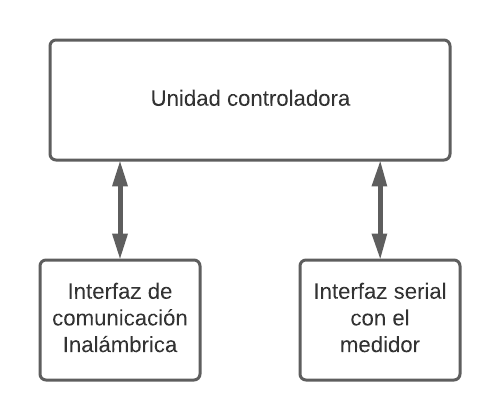
\includegraphics[width=0.5\linewidth]{img/DiagramaGeneralHardware}
	\caption{Diagrama general de los componentes del Hardware.}
	\label{fig:diagramageneralhardware}
\end{figure}

Dicho sistema requiere de una interfaz de comunicaci�n inal�mbrica debido a la necesidad de interconectar los distintos dispositivos que formar�n los nodos de la red que representar�a la parte de transmisi�n. Si se desea extraer el contador de energ�a del medidor tambi�n requiere de una interfaz serial para interactuar con este, esta ser�a la parte ,de adquisici�n de los datos.

Por �ltimo se requiere de una unidad controladora o cerebro para que se maneje el flujo de datos, el almacenamiento, tramas y dem�s rutinas necesarias para el correcto funcionamiento de las interfaces. Es de resaltar que tanto la interfaz de comunicaci�n inal�mbrica como la serial pueden funcionar como entradas y salidas de datos, para con la red y con el medidor, respectivamente. 

\section{Descripci�n del hardware}

\subsection{Interfaz de comunicaci�n inal�mbrica}

La interfaz de comunicaci�n inal�mbrica es imprescindible para este sistema. Para construir una red mallada WiFi el equipo elegido como nodo de la red debe ser compatible con esta tecnolog�a. El ESP32 tiene integrada una antena compatible con los protocolos 802.11 b/g/n y la circuiter�a necesaria para implementar y manejar este tipo de interfaz sin necesidad de otro dispositivo.

\begin{figure}[H]
	\centering
	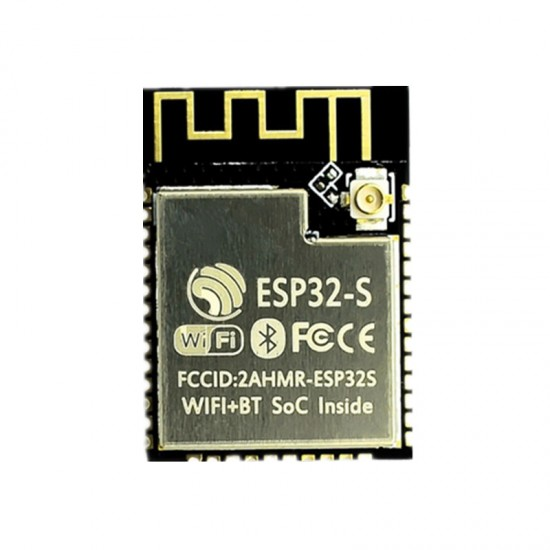
\includegraphics[width=0.4\linewidth]{img/ESP32Antenna}
	\caption{Microcontrolador ESP32 con su antena WiFi integrada.}
	\label{fig:esp32antenna}
\end{figure}

\subsection{Interfaz serial con el medidor}

El sistema debe tener la capacidad de extraer los datos de un medidor de energ�a para luego ser compartidos con el resto de la red y con el cliente externo, esta interfaz se encarga de la extracci�n de los datos. \\

Para lograr esto se debe interactuar con el medidor conectado mediante comunicaci�n serial, en la b�squeda de la mayor compatibilidad del sistema con los medidores existentes y nuevos se crearon dos 


Buscando tener la mayor compatibilidad con todos los tipos de medidores se plantea utilizar dos maneras de comunicarse con el medidor: Un bus serial y mediante la salida de calibraci�n, con estas se cubrir�a la mayor�a de los equipos.

\subsubsection{Bus serial}

Los medidores de energ�a con los que se busca compatibilidad en este apartado son los que manejan un protocolo Modbus en un bus serial RS485. Por esto se plantea utilizar un chip MAX345 que funcione como intermedio entre la comunicaci�n serial del UART del microcontrolador y el bus de campo.

\begin{figure}[H]
	\centering
	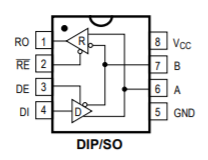
\includegraphics[width=0.4\linewidth]{img/MAX3485PinOut}
	\caption{Diagrama de pines del encapsulado DIP8 para MAX3485.}
	\label{fig:max3485pinout}
\end{figure}

El fabricante Espressif ofrece algunas sugerencias a la hora de trabajar con chip seriales para RS485, de igual forma el fabricante del chip nos ofrece un ejemplo de aplicaci�n. Como se observa en la siguientes im�genes:

\begin{figure}[H]
	\centering
	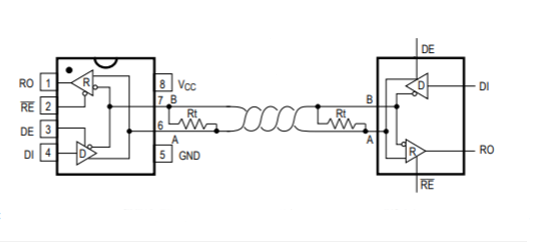
\includegraphics[width=1.0\linewidth]{img/MAX3485Bus}
	\caption{Configuraci�n recomendada por el fabricante del chip.}
	\label{fig:max3485bus}
\end{figure}


\begin{figure}[H]
	\centering
	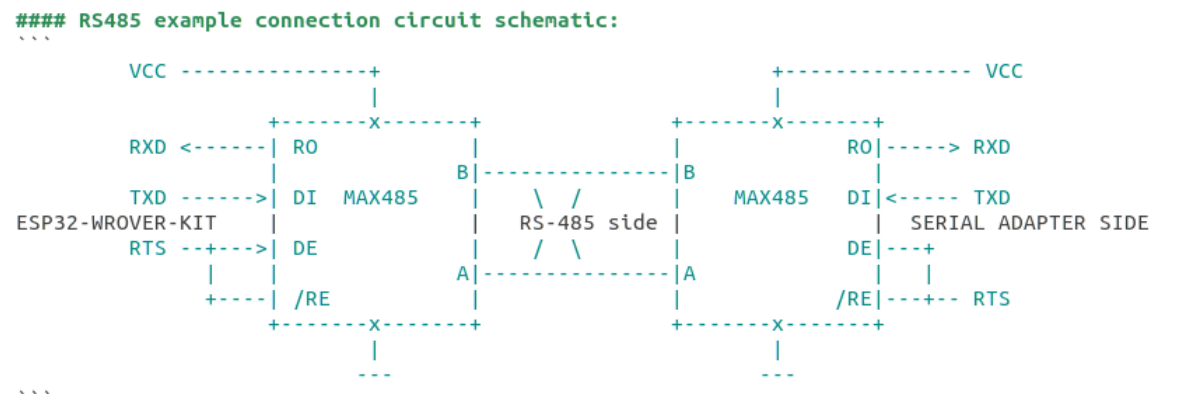
\includegraphics[width=1.1\linewidth]{img/EspressifMAX485}
	\caption{Configuraci�n recomendada por Espressif para el manejo de un chip MAX-485.}
	\label{fig:espressifmax485}
\end{figure}

La implementaci�n final es semejante a la recomendada por Espressif en \ref{fig:espressifmax485} pero colocando la resistencia RT de valor 150 Ohms como lo recomienda el fabricante del chip en \ref{fig:max3485bus}.\\

Se coloc� un condesador de  $100\;nF$ entre alimentaci�n y tierra junto con el chip MAX3485 en un circuito impreso para poder ser utilizado en la implementaci�n del prototipo del sistema, que se har� en una protoboard.

\begin{figure}[H]
	\centering
	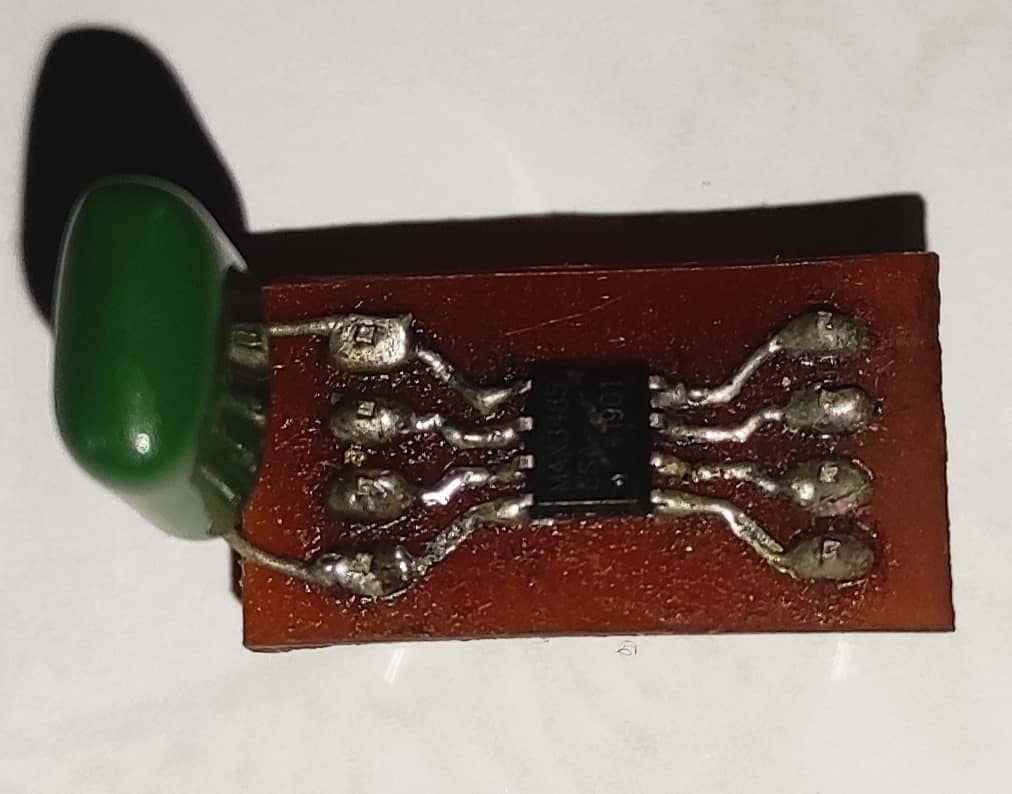
\includegraphics[width=0.4\linewidth]{img/MAX3485}
	\caption{Circuito impreso con un condensador y el chip MAX3485 utilizada para la comunicaci�n mediante el bus serial en los medidores necesarios.}
	\label{fig:max3485}
\end{figure}



\subsubsection{Salida de calibraci�n}

La salida de calibraci�n se utiliza en la fabricaci�n de los medidores para verificar y corregir el par�metro de conversi�n de imp/kWh que tiene el equipo. Esta salida suele estar formada por un optoacoplador que env�a un pulsos cada cierta fracci�n de kWh, estos pulsos se pueden captar desde la unidad controladora y aprovecharlos para extraer el conteo de energ�a. \\

Pero se deben tener en cuenta dos cosas: el medidor puede tener una condici�n inicial de energ�a que no se captar� y, de ocurrir una falla de alimentaci�n se perder� la cuenta que se lleva si no se guarda de manera permanente. Ambos problemas se tratar�n mediante el software y se explicar� la soluci�n propuesta m�s adelante.

Para utilizar dicha salida se utiliza un transistor y una resistencia de pull-up para evitar da�ar las entradas del microcontrolador con un voltaje o corriente mayor a la soportada.

\begin{figure}[H]
	\centering
	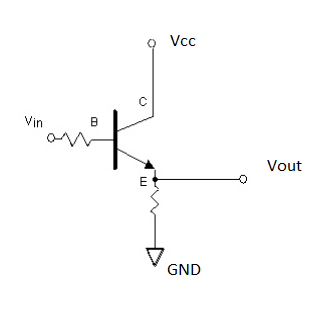
\includegraphics[width=0.5\linewidth]{img/SeguidorEmisor}
	\caption{Topolog�a seguidor de emisor utilizada en la salida optoacoplada del medidor de energ�a.}
	\label{fig:seguidoremisor}
\end{figure}


\subsection{Unidad controladora}

La unidad controladora es la encargada de: gestionar el estado del nodo en la red mallada, recibir y transmitir los datos, controlar los perif�ricos para enviar el mensaje necesario a trav�s de la interfaz serial al medidor y adem�s de comunicarse enviar al exterior de la red mallada el resultado de esta adquisici�n de los datos.  

\begin{figure}[H]
	\centering
	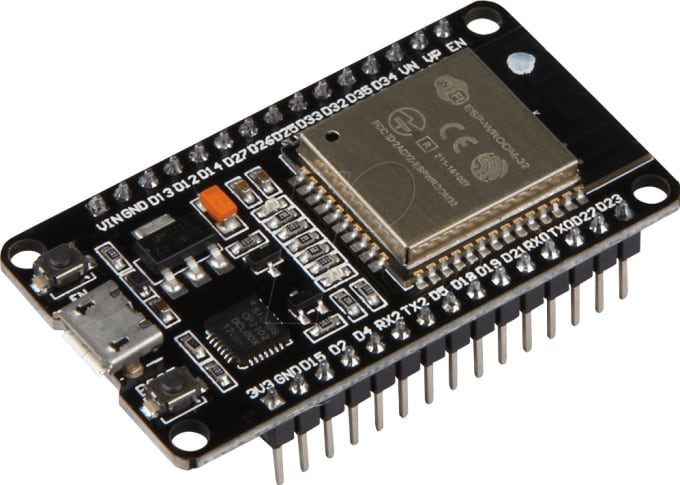
\includegraphics[width=0.4\linewidth]{img/UnidadControladora}
	\caption{Unidad controladora del sistema, tarjeta de desarrollo ESP32.}
	\label{fig:unidadcontroladora}
\end{figure}

El cerebro de cada nodo tiene muchas tareas pero no todas se ejecutan al mismo tiempo, muchas dependen del nodo y de la configuraci�n que se le de a este mediante el software. La forma de manejar de manera correcta las tareas en cada nodo ser� ilustrada en el siguiente capitulo.

%

%==================================================================
\chapter{DEFINICI�N Y DESCRIPCI�N DEL HARDWARE}\label{CAP:hard}
%\markboth{Tu Segundo Cap?tulo}{Tu Segundo Cap?tulo}%
% !TeX encoding = ISO-8859-1
% !TeX spellcheck = es_ES

\section{Definici�n del hardware}

Un sistema de adquisici�n y transmisi�n de datos orientado a medidores de energ�a, debe contar con varios elementos que, interconectados, lleven a un funcionamiento general.

\begin{figure}[H]
	\centering
	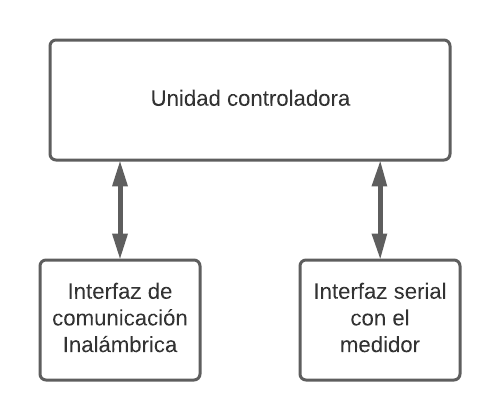
\includegraphics[width=0.5\linewidth]{img/DiagramaGeneralHardware}
	\caption{Diagrama general de los componentes del Hardware.}
	\label{fig:diagramageneralhardware}
\end{figure}

Dicho sistema requiere de una interfaz de comunicaci�n inal�mbrica debido a la necesidad de interconectar los distintos dispositivos que formar�n los nodos de la red que representar�a la parte de transmisi�n. Si se desea extraer el contador de energ�a del medidor tambi�n requiere de una interfaz serial para interactuar con este, esta ser�a la parte ,de adquisici�n de los datos.

Por �ltimo se requiere de una unidad controladora o cerebro para que se maneje el flujo de datos, el almacenamiento, tramas y dem�s rutinas necesarias para el correcto funcionamiento de las interfaces. Es de resaltar que tanto la interfaz de comunicaci�n inal�mbrica como la serial pueden funcionar como entradas y salidas de datos, para con la red y con el medidor, respectivamente. 

\section{Descripci�n del hardware}

\subsection{Interfaz de comunicaci�n inal�mbrica}

La interfaz de comunicaci�n inal�mbrica es imprescindible para este sistema. Para construir una red mallada WiFi el equipo elegido como nodo de la red debe ser compatible con esta tecnolog�a. El ESP32 tiene integrada una antena compatible con los protocolos 802.11 b/g/n y la circuiter�a necesaria para implementar y manejar este tipo de interfaz sin necesidad de otro dispositivo.

\begin{figure}[H]
	\centering
	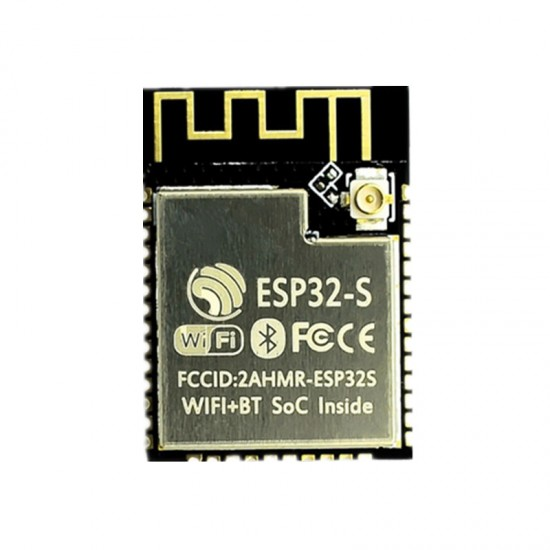
\includegraphics[width=0.4\linewidth]{img/ESP32Antenna}
	\caption{Microcontrolador ESP32 con su antena WiFi integrada.}
	\label{fig:esp32antenna}
\end{figure}

\subsection{Interfaz serial con el medidor}

El sistema debe tener la capacidad de extraer los datos de un medidor de energ�a para luego ser compartidos con el resto de la red y con el cliente externo, esta interfaz se encarga de la extracci�n de los datos. \\

Para lograr esto se debe interactuar con el medidor conectado mediante comunicaci�n serial, en la b�squeda de la mayor compatibilidad del sistema con los medidores existentes y nuevos se crearon dos 


Buscando tener la mayor compatibilidad con todos los tipos de medidores se plantea utilizar dos maneras de comunicarse con el medidor: Un bus serial y mediante la salida de calibraci�n, con estas se cubrir�a la mayor�a de los equipos.

\subsubsection{Bus serial}

Los medidores de energ�a con los que se busca compatibilidad en este apartado son los que manejan un protocolo Modbus en un bus serial RS485. Por esto se plantea utilizar un chip MAX345 que funcione como intermedio entre la comunicaci�n serial del UART del microcontrolador y el bus de campo.

\begin{figure}[H]
	\centering
	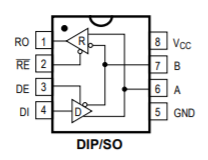
\includegraphics[width=0.4\linewidth]{img/MAX3485PinOut}
	\caption{Diagrama de pines del encapsulado DIP8 para MAX3485.}
	\label{fig:max3485pinout}
\end{figure}

El fabricante Espressif ofrece algunas sugerencias a la hora de trabajar con chip seriales para RS485, de igual forma el fabricante del chip nos ofrece un ejemplo de aplicaci�n. Como se observa en la siguientes im�genes:

\begin{figure}[H]
	\centering
	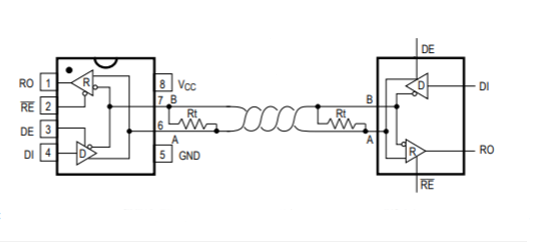
\includegraphics[width=1.0\linewidth]{img/MAX3485Bus}
	\caption{Configuraci�n recomendada por el fabricante del chip.}
	\label{fig:max3485bus}
\end{figure}


\begin{figure}[H]
	\centering
	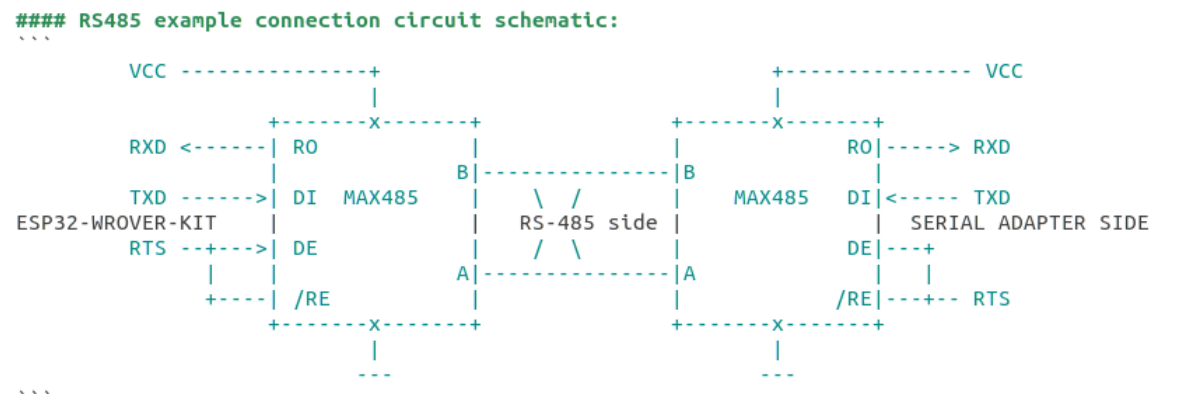
\includegraphics[width=1.1\linewidth]{img/EspressifMAX485}
	\caption{Configuraci�n recomendada por Espressif para el manejo de un chip MAX-485.}
	\label{fig:espressifmax485}
\end{figure}

La implementaci�n final es semejante a la recomendada por Espressif en \ref{fig:espressifmax485} pero colocando la resistencia RT de valor 150 Ohms como lo recomienda el fabricante del chip en \ref{fig:max3485bus}.\\

Se coloc� un condesador de  $100\;nF$ entre alimentaci�n y tierra junto con el chip MAX3485 en un circuito impreso para poder ser utilizado en la implementaci�n del prototipo del sistema, que se har� en una protoboard.

\begin{figure}[H]
	\centering
	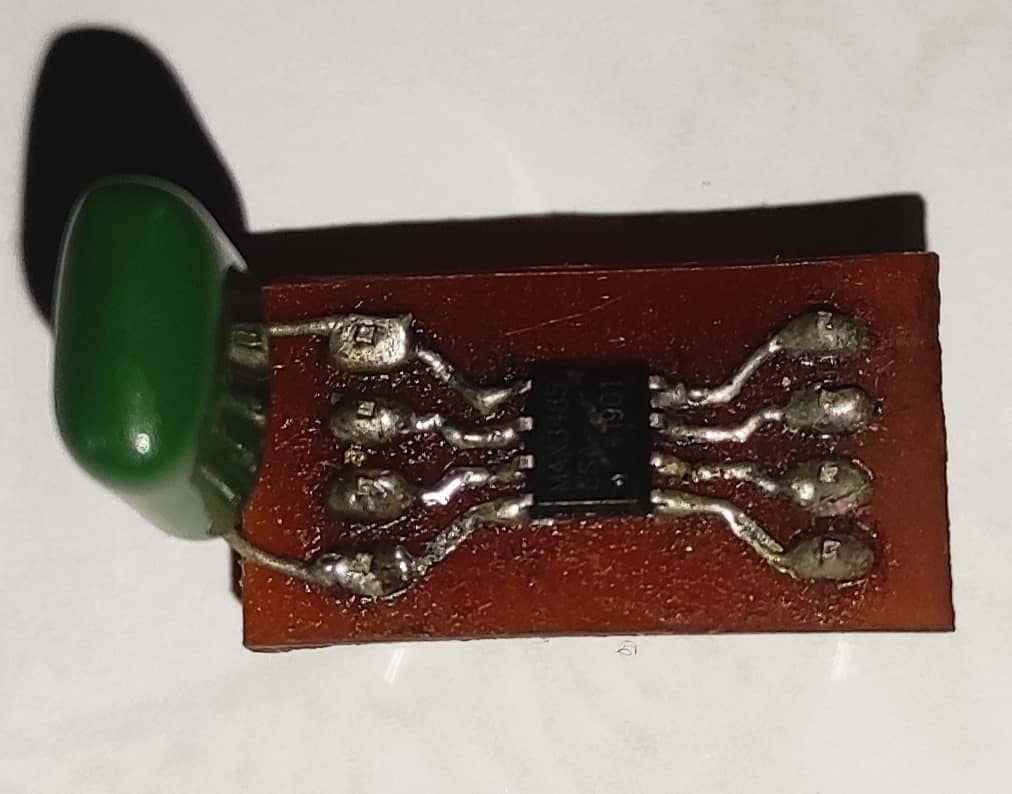
\includegraphics[width=0.4\linewidth]{img/MAX3485}
	\caption{Circuito impreso con un condensador y el chip MAX3485 utilizada para la comunicaci�n mediante el bus serial en los medidores necesarios.}
	\label{fig:max3485}
\end{figure}



\subsubsection{Salida de calibraci�n}

La salida de calibraci�n se utiliza en la fabricaci�n de los medidores para verificar y corregir el par�metro de conversi�n de imp/kWh que tiene el equipo. Esta salida suele estar formada por un optoacoplador que env�a un pulsos cada cierta fracci�n de kWh, estos pulsos se pueden captar desde la unidad controladora y aprovecharlos para extraer el conteo de energ�a. \\

Pero se deben tener en cuenta dos cosas: el medidor puede tener una condici�n inicial de energ�a que no se captar� y, de ocurrir una falla de alimentaci�n se perder� la cuenta que se lleva si no se guarda de manera permanente. Ambos problemas se tratar�n mediante el software y se explicar� la soluci�n propuesta m�s adelante.

Para utilizar dicha salida se utiliza un transistor y una resistencia de pull-up para evitar da�ar las entradas del microcontrolador con un voltaje o corriente mayor a la soportada.

\begin{figure}[H]
	\centering
	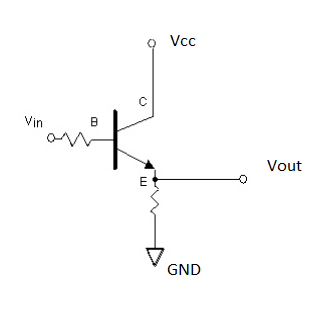
\includegraphics[width=0.5\linewidth]{img/SeguidorEmisor}
	\caption{Topolog�a seguidor de emisor utilizada en la salida optoacoplada del medidor de energ�a.}
	\label{fig:seguidoremisor}
\end{figure}


\subsection{Unidad controladora}

La unidad controladora es la encargada de: gestionar el estado del nodo en la red mallada, recibir y transmitir los datos, controlar los perif�ricos para enviar el mensaje necesario a trav�s de la interfaz serial al medidor y adem�s de comunicarse enviar al exterior de la red mallada el resultado de esta adquisici�n de los datos.  

\begin{figure}[H]
	\centering
	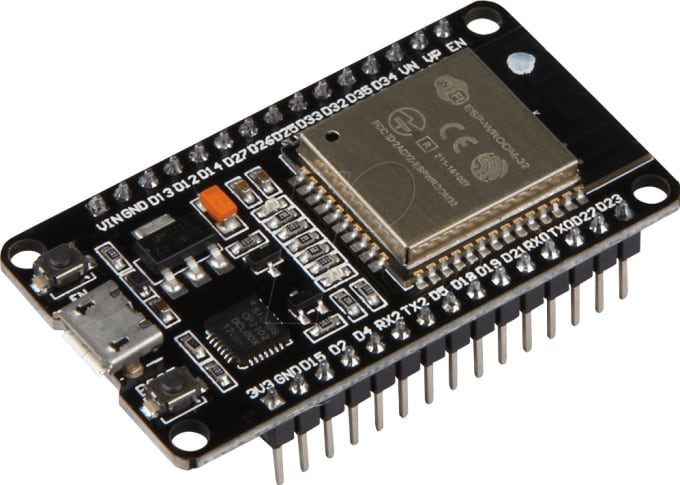
\includegraphics[width=0.4\linewidth]{img/UnidadControladora}
	\caption{Unidad controladora del sistema, tarjeta de desarrollo ESP32.}
	\label{fig:unidadcontroladora}
\end{figure}

El cerebro de cada nodo tiene muchas tareas pero no todas se ejecutan al mismo tiempo, muchas dependen del nodo y de la configuraci�n que se le de a este mediante el software. La forma de manejar de manera correcta las tareas en cada nodo ser� ilustrada en el siguiente capitulo.

%

%==================================================================
\chapter{DEFINICI�N Y DESCRIPCI�N DEL SOFTWARE}\label{CAP:soft}
%\markboth{Tu Segundo Cap?tulo}{Tu Segundo Cap?tulo}%
% !TeX encoding = ISO-8859-1
% !TeX spellcheck = es_ES

\section{Definici�n del software}

Para el objetivo planteado en este proyecto, se requiere el uso de un microcontrolador por lo que se debe implementar un programa o firmware para configurar y utilizar, de manera correcta, los perif�ricos correspondientes a las conexiones inal�mbricas y el manejo de datos seriales; adem�s es necesario un protocolo de conexi�n hacia un agente externo que permita enviar los datos recolectados por la infraestructura, una infraestructura que debe ser creada mediante este firmware y como m�todo de configuraci�n de los nodos una interfaz gr�fica de usuario (GUI) que le permita a la red adaptarse de manera sencilla al lugar donde se instale.\\

\begin{figure}[H]
	\centering
	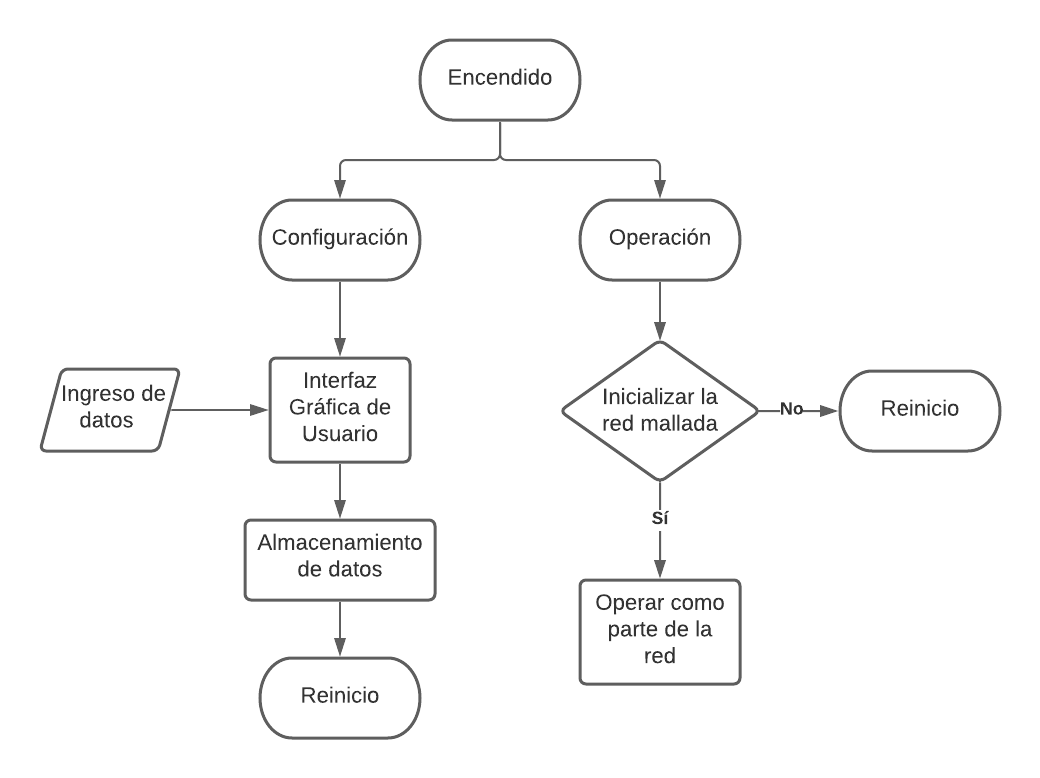
\includegraphics[width=1.0\linewidth]{img/DiagramaGenerico}
	\caption{Diagrama de bloques gen�rico del sistema}
	\label{fig:diagramageneralsoft}
\end{figure}


El firmware en el microcontrolador (ESP32) debe ser capaz de iniciar en dos modos: el modo de operaci�n y el modo de configuraci�n. El modo de inicio debe ser controlado por el usuario.\\


La rutina de configuraci�n debe ofrecer al usuario una interfaz gr�fica donde se pueda modificar todos los par�metros que sean necesarios para establecer la conexi�n con el punto de acceso local, del mismo modo se debe conectar la red con el agente externo y realizar el env�o de datos; los par�metros de funcionamiento de la parte serial de cada nodo para extraer desde los medidores la informaci�n y los necesarios en la red mallada para establecer la cantidad de conexiones y el registro de nodos en la red; adem�s del usuario y contrase�a de acceso a dicha p�gina.\\


Por otra parte, la rutina de configuraci�n debe detenerse en caso de que faltase alg�n par�metro fundamental para el funcionamiento, en caso contrario debe ir activando etapa por etapa los procesos para: configurar los perif�ricos necesarios, activar la conexi�n inal�mbrica, conectarse con el punto de acceso y registrarse en la red mallada.\\


Las operaciones anteriores son compartidas en todos los nodos y son necesarias para entrar en la red. Las siguientes rutinas a ejecutarse dependen de la jerarqu�a que posee el nodo en la red mallada y de la funci�n que se haya configurado para el nodo en la interfaz gr�fica. La jerarqu�a que tiene un nodo depender� de la intensidad de se�al de este respecto al punto de acceso.\\

En caso de ser el nodo de mayor jerarqu�a, dicho nodo ser� el encargado de gestionar la comunicaci�n de la red con el exterior, este nodo servir� como el enlace para enviar y recibir la informaci�n para toda la red. Adem�s a partir de este nodo se formar� el resto de la topolog�a de red mallada.\\

Los dem�s nodos deben ser repetidores para que la se�al pueda abarcar el espacio f�sico necesario o nodos conectados a medidores para la extracci�n de datos. Estas dos rutinas no deben ser excluyentes, los nodos deben tener la capacidad de ser repetidores y extraer datos al mismo tiempo.\\

Hay dos rutinas principales para la extracci�n de datos, una mediante la salida de calibraci�n del medidor y otra que se conecta a un bus serial RS485. La rutina de extracci�n de datos debe estar configurada para que se utilice el m�todo necesario seg�n el medidor. En caso de que los datos sean extra�dos por la salida de calibraci�n del medidor se debe dise�ar una rutina para contar y almacenar los pulsos que esta genera considerando la cantidad inicial de kWh, esto por ser el registro que se desea transmitir debe estar almacenado de manera persistente y debe estar protegido contra p�rdidas de alimentaci�n. Por el contrario si en el nodo los datos son adquiridos mediante un bus serial, la persistencia de datos es realizada por el medidor, entonces la rutina en este caso solo debe encargarse de la trama serial. En ambos casos una vez adquiridos los datos se deben enviar a la red exterior cuando sean solicitados.

\section{Descripci�n del software}

\begin{figure}[H]
	\centering
	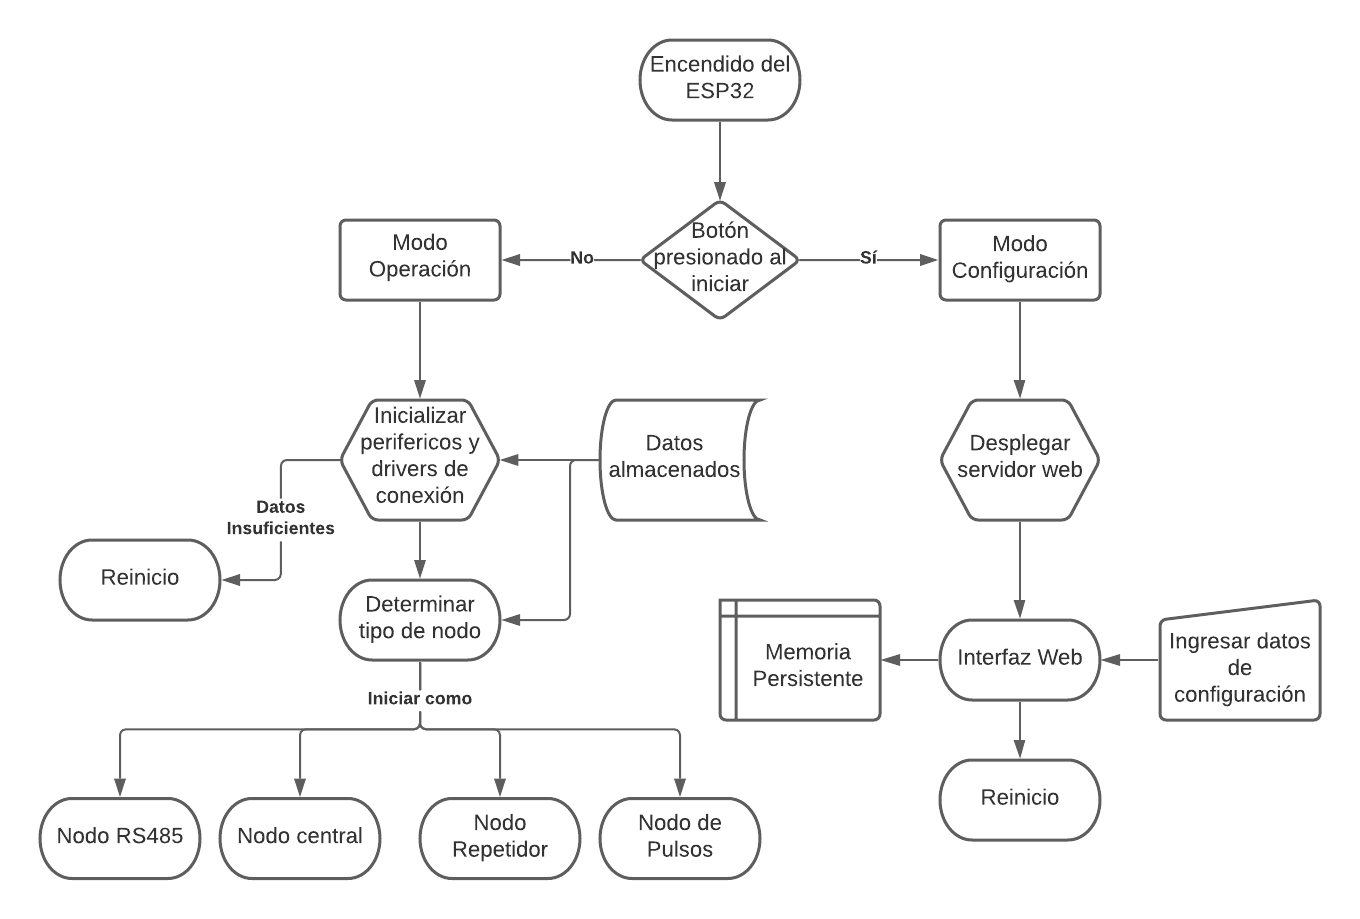
\includegraphics[width=1.0\linewidth]{img/DiagramaGeneral.png}
	\caption{Diagrama general de funcionamiento ilustrado.}
	\label{fig:diagramageneral}
\end{figure}

\subsection{Modo de configuraci�n}

El modo de configuraci�n utiliza un sistema de archivos para implementar un servidor web que soporta protocolos http. Este sistema de archivos en el microcontrolador se trabaja con la API de \textit{SPIFFS} que ofrece el fabricante, esto permite grabar en la memoria flash del microcontrolador los diferentes archivos necesarios para implementar una p�gina web como interfaz gr�fica de usuario. Sin embargo para que esto ocurra se requiere en la configuraci�n de inicio definir un espacio en una tabla de particiones para toda esta estructura.

\subsubsection{Tablas de particiones en el ESP32}

Un c�digo cualquiera en el ESP32 puede contener m�ltiples aplicaciones, as� como muchos tipos diferentes de datos (datos de calibraci�n, sistemas de archivos, almacenamiento de par�metros, etc.) es por esto que las tablas de particiones se encuentran con un offset para cada c�digo en cuesti�n en la memoria flash.

En cada grabado se utiliza un archivo de tabla de particiones por defecto que es definida en el men� de configuraciones tambi�n llamado \textit{menuconfig}, hay dos tablas modelos para utilizar en este men�: \textit{Aplicaci�n �nica de f�brica} (\ref{Tab:Partition_Table_example}) y \textit{Aplicaci�n de dos definiciones}. La diferencia entre ambas tablas radica en la cantidad de particiones en la memoria flash y c�mo son utilizadas: La aplicaci�n �nica solo posee un c�digo para arranque de tipo \textit{app} en la tabla de particiones, mientras que la tabla de dos definiciones posee dos c�digos para iniciar el micro y es el gestor de arranque mediante ciertas reglas el que decide cu�l data de tipo \textit{app} poner en marcha. Este �ltimo modelo de tabla es �til cuando se quiere incorporar actualizaciones inal�mbricas del programa en el micro tambi�n llamadas \textit{Over The Air updates (OTA)}.\\

\begin{figure}[H]
	\centering
	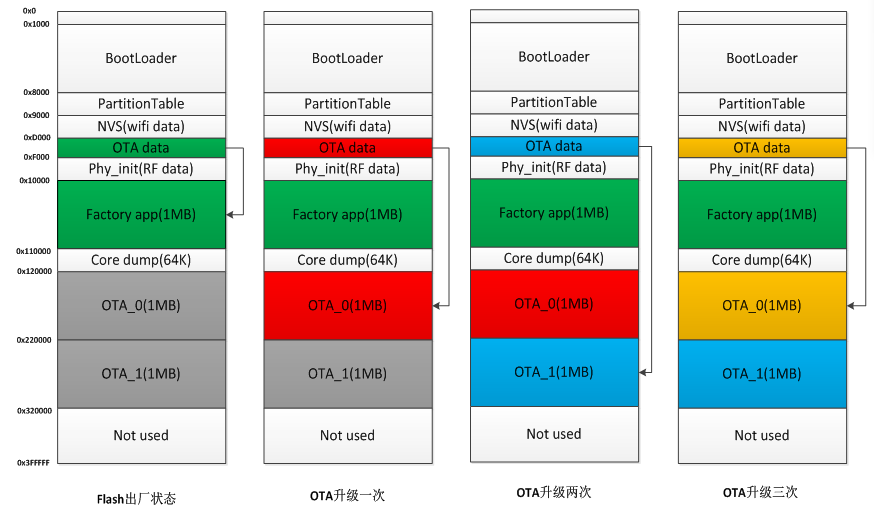
\includegraphics[width=0.7\linewidth]{img/TablasOTA}
	\caption{Diagrama ilustrativo de la memoria flash para los modelos de tablas de partici�n. Columna 1: Aplicaci�n de f�brica. Columna 2, 3, 4: Aplicaciones con arranques m�ltiples}
	\label{fig:tablasota}
\end{figure}

En este proyecto se utiliza una aplicaci�n �nica sin actualizaciones inal�mbricas por lo que se utiliz� el primer modelo de tabla, cuyas estructuras en archivo CSV se especifican a continuaci�n:

\begin{table}[H]
	\centering
	\caption{ESP-IDF Tabla de Particiones por defecto (Aplicaci�n �nica de f�brica, sin OTA)}
	\label{Tab:Partition_Table_example}
	\medskip
	\begin{tabular}{llllll}
		\toprule
		Name & Type & SubType & Offset & Size & Flags\\
		\midrule
		nvs &      data& nvs&    0x9000&  0x6000 & \\
		phyinit& data& phy& 0xf000& 0x1000& \\
		factory&  app&  factory& 0x10000& 1M& \\	
		\bottomrule
	\end{tabular}
\end{table}

Con un desplazamiento de 0x10000 (64KB) en la flash, se encuentra la aplicaci�n llamada "f�brica". El gestor de arranque ejecutar� esta aplicaci�n de forma predeterminada. Tambi�n hay dos regiones de datos definidas en la tabla de particiones para almacenar la partici�n de la biblioteca \textit{NVS} y los datos de inicio \textit{PHY} (datos de calibraci�n de perif�ricos).\\

Con la finalidad de adaptarse a la aplicaci�n fue necesario modificar la tabla de particiones puesto que la interfaz gr�fica de m�do de configuraci�n y las diferentes particiones para datos requer�an de un tama�o mayor al que posee la tabla de particiones original. Para crear o modificar los tama�os en una partici�n basta con configurar en el \textit{menuconfig} del proyecto que se utilizar� una tabla de particiones personalizada.

%\textbf{Explicaci�n de particiones de memoria para configuraci�n, operaci�n y memoria rotativa}

%Al iniciar el programa se configuran los perif�ricos necesarios mediante las API que ofrece el fabricante \href{https://docs.espressif.com/projects/esp-idf/en/latest/esp32/api-reference/index.html}{\textit{Espressif Systems}} para el ESP32.


	\begin{table}[H]
	\centering
	\caption{Tabla de particiones personalizada para la aplicaci�n}
	\label{Tab:Partition_table_web}
	\medskip
	\begin{tabular}{llllll}
		\toprule
		Name & Type & SubType & Offset & Size & Flags\\
		\midrule
		nvs &      data& nvs&    0x9000&  0x6000 & \\
		phyinit& data& phy& 0xf000& 0x1000& \\
		factory&  app&  factory& 0x10000& 1M& \\
		www& data& spiffs& &1M&\\
		.& .& .& &.&\\
		.& .& .& &.&\\
		.& .& .& &.&\\
		\bottomrule
	\end{tabular}
\end{table}


La columna \textit{Name} y la fila \textit{www} de este archivo separado por comas representado en la tabla \ref{Tab:Partition_table_web} se define el espacio de memoria donde se guardaran todos los archivos necesarios para la p�gina web, el \textit{Type} es data y el \textit{SubType} es \textit{spiffs} debido a que as� se debe definir en la memoria el tipo de datos para un sistema de archivos. Y el espacio en la memoria es de 1MB como lo dice en la columna \textit{Size}.\\

El servidor \textit{HTTP} est� implementado por el fabricante en los ejemplos de aplicaciones, se tomo dicha API y se adapt� a las necesidades de esta aplicaci�n. 

\subsubsection{Interfaz Gr�fica de usuario}

La interfaz gr�fica consta de 5 pantallas, cada una con un formulario que son par�metros necesarios para conectarse a la red mallada, para su funcionamiento como alg�n tipo de nodo o para la conexi�n con el enrutador. A la interfaz se accede mediante la direcci�n IP del nodo o mediante un DNS relacionado con la MAC. Tambi�n se incluye la configuraci�n de usuario y clave para proteger al acceso, de usuarios no deseados. Las pantallas por las que puede ingresar datos el usuario son:

\begin{enumerate}
	\item \textbf{Inicio de sesi�n}
	
	El inicio de sesi�n requiere al menos de un usuario y contrase�a para autenticar el acceso a la configuraci�n del sistema. Esta pantalla debe ofrecer el acceso al sistema de configuraci�n si estos son introducidos correctamente y rechazarlos en caso de que no.\\
	
	
	\item \textbf{Par�metros de red mallada}
	
	La pantalla de ingreso de los par�metros para la red mallada requiere tener los siguientes par�metros: 
	\begin{itemize}
		\item ID de la red: Que es el identificador de la red, es un par�metro parecido en formato a una direcci�n MAC que permite identificar la red mallada y diferenciarla de otras implementadas.
		\item Contrase�a de la red: Es la clave requerida por los nodos para ingresar a la red. Sin este par�metro y el anterior no ser�n admitidos en la red mallada.
		\item Cantidad m�xima de capas: Se refiere a la cantidad de capas aceptadas por la red, este par�metro es necesario para la configuraci�n de la misma. El valor var�a entre 1 y 25 pero el fabricante recomienda 10 para tiempos de retardos manejables.
		\item Cantidad m�xima de estaciones conectadas: Este par�metro es el n�mero m�ximo de estaciones WiFi conectadas que tendr� el nodo, en t�rminos de la red mallada es la cantidad m�xima de nodos hijo que puede tener un nodo. Se aceptan valores entre 1 y 10 pero recomienda que sea menor que 6 para un buen funcionamiento del punto de acceso.
		\item Puerto del socket: El n�mero de puerto TCP/IP que ser� abierto por el microcontrolador para conexiones externas, esto ser� explicado en detalle en la rutina correspondiente a este proceso.\\
		
	\end{itemize}


	\item \textbf{Par�metros seriales}
	
	La pantalla de ingreso de los par�metros para el funcionamiento serial debe depender del tipo de nodo que se busque configurar puesto que hay al menos 3 tipos de nodos en la red sin contar el nodo central. En general para cualquier tipo de nodo los par�metros necesarios son:
	
	\begin{itemize}
		\item Tasa de baudios: La tasa de comunicaci�n con el medidor � el bus serial.
		\item Factor de conversi�n [$\frac{imp}{kWh}$]: La cantidad de impusos por cada kWh de energ�a registrada por el medidor al que se conecte el nodo.
		\item Condici�n inicial de energ�a: Al soportar medidores ya instalado se deben tomar en cuenta las condiciones iniciales de energ�a consumida que marca el medidor para que el sistema sea coherente con el equipo.
		\item Identificador de esclavo: Necesario para identificar el tipo de nodo que emular� un bus serial.\\
		
	\end{itemize}
	
	\item \textbf{Configuraci�n de red local}
	
	Esta vista debe contemplar el ingreso de los par�metros de SSID y contrase�a de la red local.\\
	
	
	\item \textbf{Configuraci�n de inicio de sesi�n}
	
	Esta vista responde a la necesidad de cambiar el nombre y la contrase�a por defecto para el acceso al sistema de configuraci�n mediante la interfaz web gr�fica.\\
	
\end{enumerate}

\subsection{Modo de operaci�n}

En este modo el primer perif�rico en configurarse en cualquiera de los nodos es la memoria no vol�til (NVS), tambi�n llamada memoria flash, que se utiliza para almacenar informaci�n persistente entre reinicios del microcontrolador. El fabricante ofrece una interfaz de programaci�n de aplicaciones (%Link a la API de NVS
) que permite configurarla y operar f�cilmente con esta.

Esto se debe a que ah� se almacenan todos los datos que se transmiten al microcontrolador mientras este se encuentra en el modo de configuraci�n. 

Se toma desde la memoria flash la informaci�n sobre el tipo de nodo (serial RS485, entrada por pulsos o repetidor) y todos los par�metros que vienen asociados a este (tasa de baudios, ID serial, kWh iniciales, etc.), as� como los par�metros necesarios para registrarse en la red mallada y poder comunicarse a trav�s de la red.

Luego se debe configurar el WiFi en cada uno de los medidores para poder unirse a la red mallada. Este perif�rico en el ESP32 posee tambi�n una interfaz de programaci�n de aplicaciones para programarlo de manera m�s sencilla (%Link a la API del WiFi
). Mediante esta interfaz, se calibra el WiFi, se asigna un lugar para almacenar sus par�metros de calibraci�n y se coloca el modo de operaci�n. El ESP32 posee tres modos de operaci�n para este perif�rico: estaci�n (STA), punto de acceso (AP) y un modo h�brido (AP/STA). Este �ltimo es el que se suele utilizar en la red mallada. Una vez configurado el WiFi se procede con la configuraci�n e inicio de la red mallada.

\subsubsection{La red mallada y el nodo central}

La topolog�a de red mallada utilizada en el proyecto est� basada en la que provee \textit{Espressif} para ser utilizada en conjunto con el ESP32. Dicha topolog�a es llamada ESP-MESH y el fabricante proporciona una interfaz de programaci�n de aplicaciones (%API de ESP-MESH
) para interactuar y modificar dicha topolog�a con la intenci�n de que sea adaptable a las soluciones que se deseen implementar. Seg�n el tipo de medidor que haya sido configurado en la interfaz web ser�n activadas unas tareas u otras, puesto que cada medidor requiere de diferentes procesos para extraer y transmitir sus datos. 
\\

El objetivo es implementar una red mallada que transmita una informaci�n representativa de la cantidad de energ�a consumida, tom�ndola a partir de medidores de energ�a. Esta arquitectura de red requiere de un nodo particular para comunicarse hacia redes externas, llamado nodo ra�z o nodo \textit{root}. Dicho nodo se elige mediante par�metros de calidad de se�al, espec�ficamente se tiene en cuenta la intensidad de se�al (RSSI) de cada nodo con el enrutador. Considerando esto se efect�a una votaci�n en la cual se elige qu� nodo ser� asignado como nodo ra�z, este suele ser el nodo de mayor intensidad de se�al pues esto garantiza una comunicaci�n estable.

\begin{figure}[H]
	\centering
	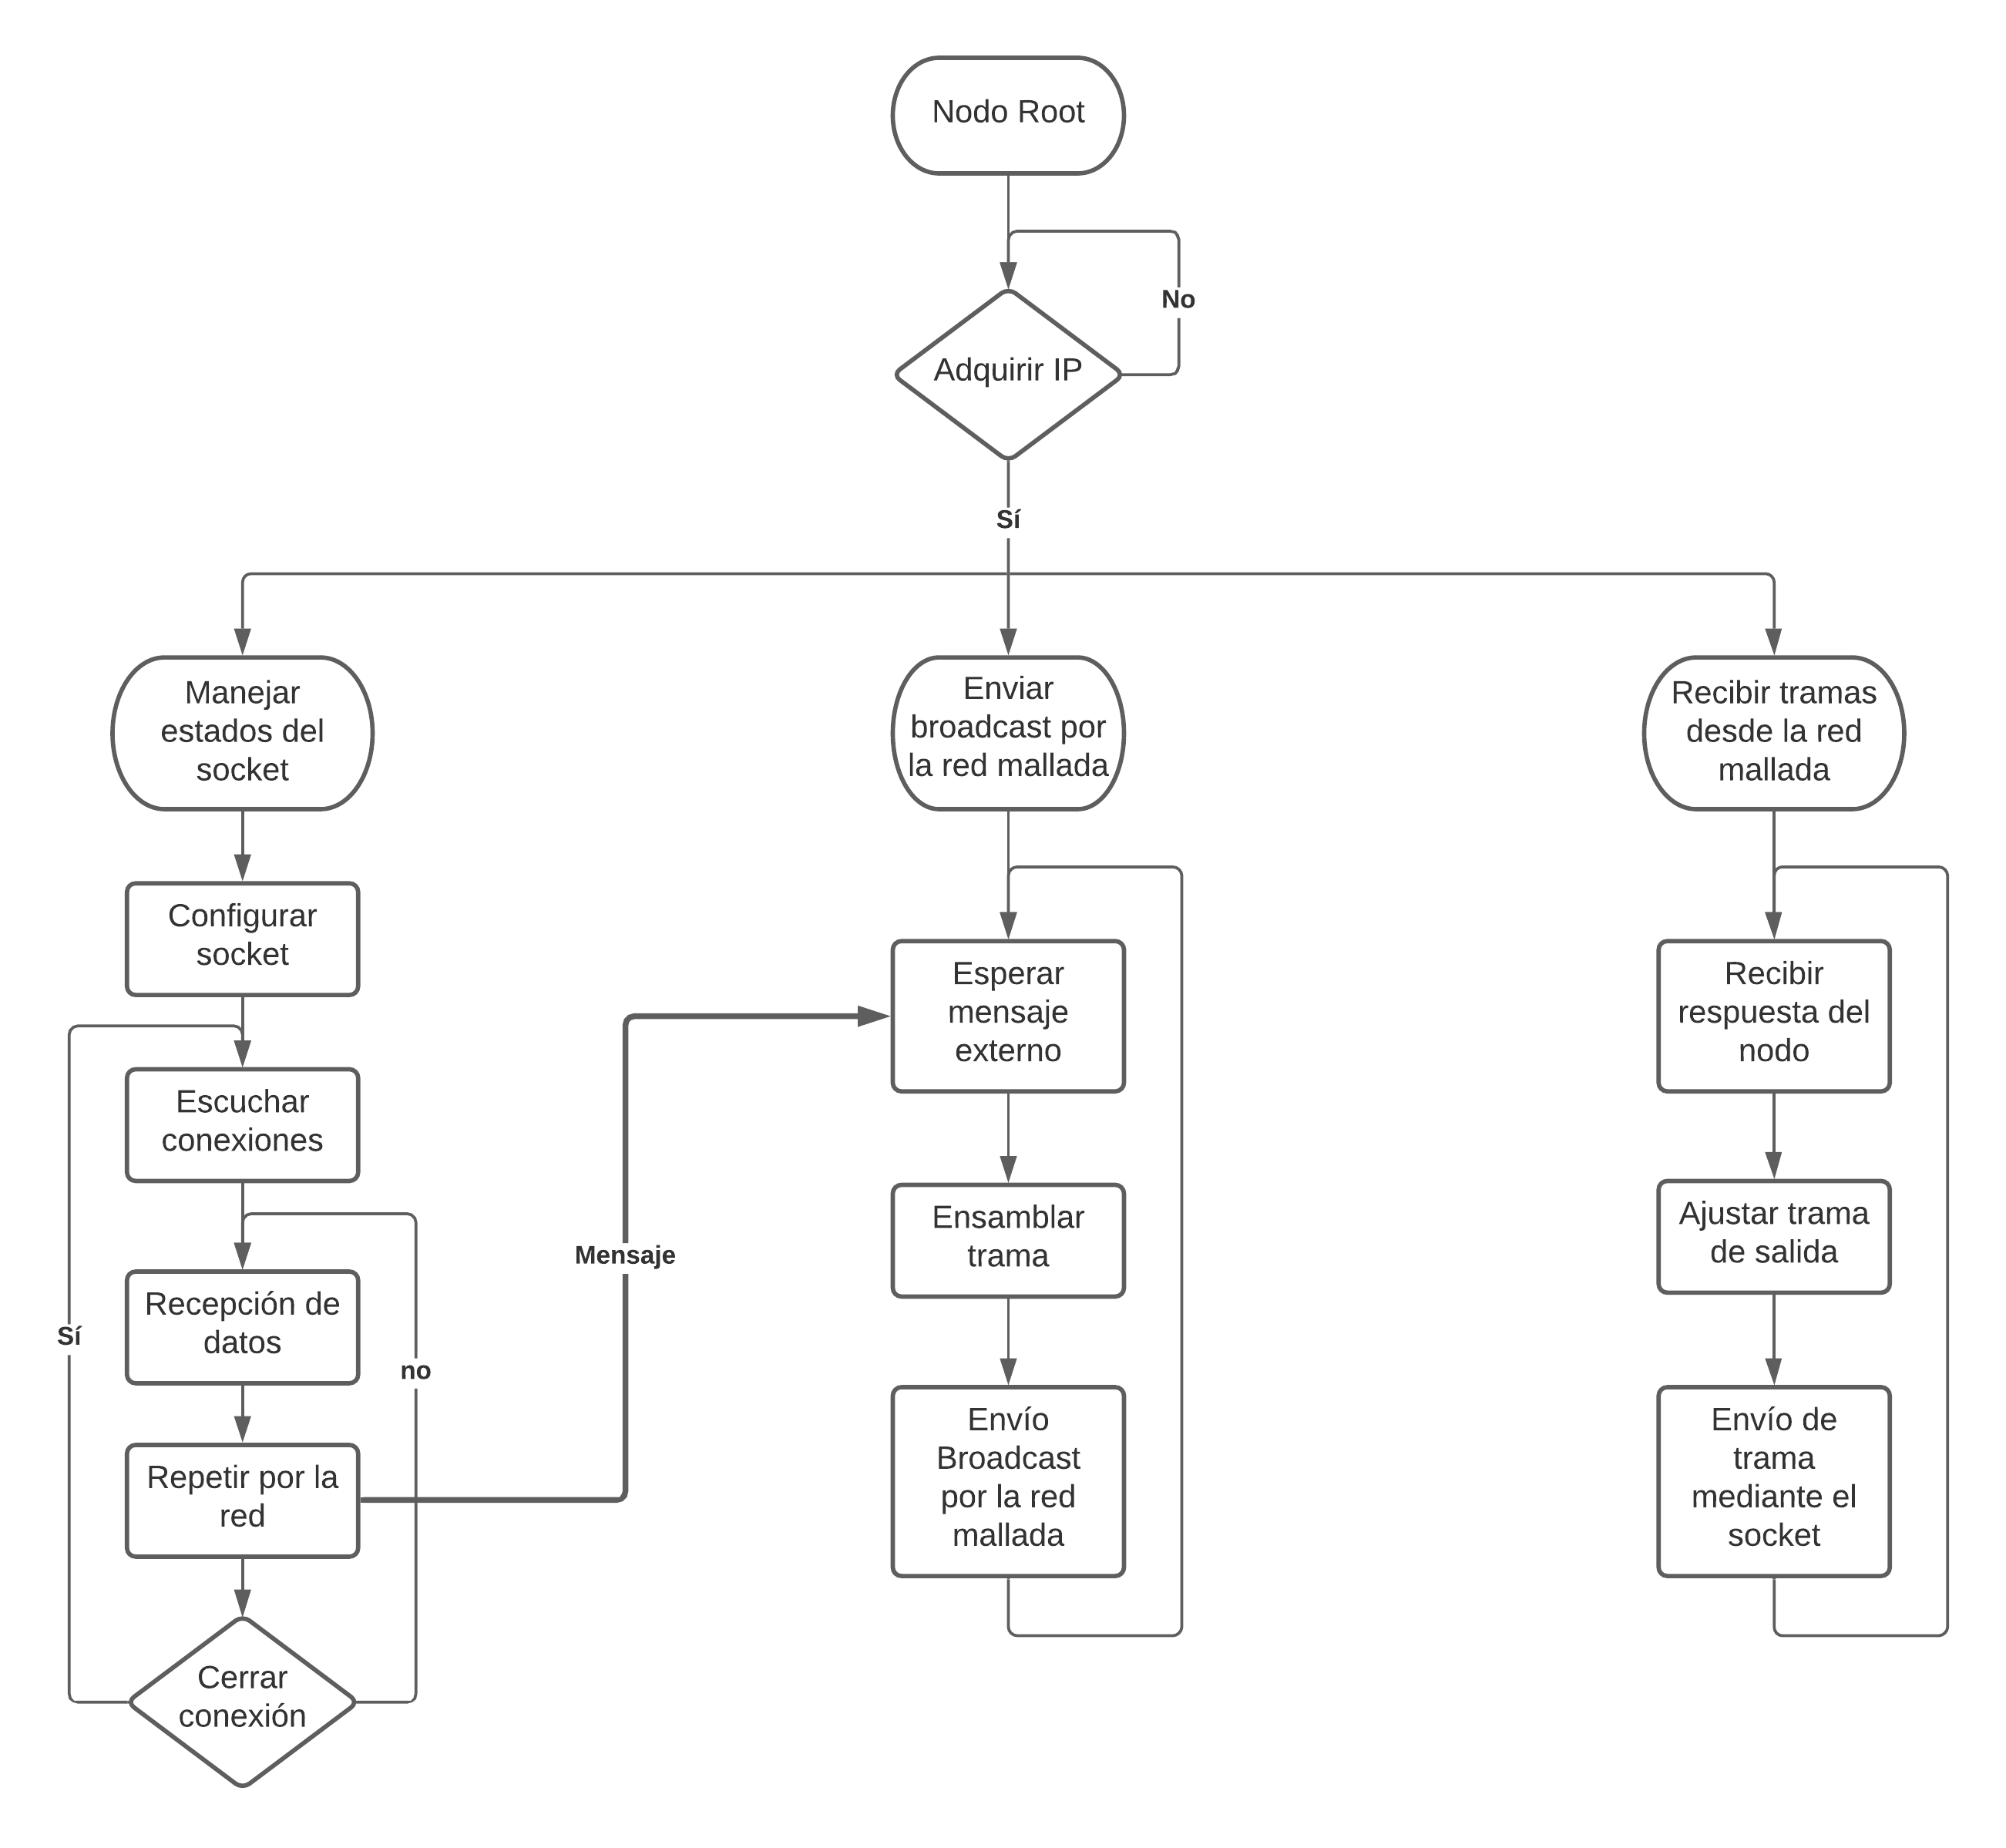
\includegraphics[width=1.0\linewidth]{img/NodoRoot}
	\caption{Diagrama de flujo de las tareas implementadas en el nodo central.}
	\label{fig:nodoroot}
\end{figure}

Una vez elegido este nodo comienza a ejecutarse el c�digo con las tareas implementadas en la programaci�n para �l. Son tres tareas, sin embargo debe comenzar estableciendo la conexi�n WiFi con el enrutador y obteniendo la IP de parte del DHCP del enrutador. Esta direcci�n asignada es la que ser� utilizada para comunicarse con la red mallada desde una red exterior.\\

Una vez se obtiene la IP se crean en el RTOS las tareas necesarias para el nodo central:
\begin{itemize}
	\item \textbf{Manejar estados del socket:} El sistema requiere un punto de conexi�n que sirva como entrada y salida para los datos requeridos. Un socket ofrece una manera de intercambiar un flujo de datos y permite enviar mensajes a otra direcci�n IP.\\
	
	Dicho socket requiere de un proceso de configuraci�n para el que se utiliza inicialmente un n�mero de puerto. Este puerto ser� habilitado para permitir conexiones entrantes de clientes que soporten esta estructura de socket y el protocolo inherente a este bien sea TCP o UDP. Se utiliz� el protocolo TCP ya que este protocolo de transporte garantiza la integridad de los datos. \\
	
	Una vez establecidos el puerto y el protocolo a soportar, el socket queda en espera de conexiones entrantes. Cuando un cliente solicita conectarse y el socket no est� ocupado por otro cliente, esta conexi�n es aceptada y se cambia el estado a \textit{esperar mensaje}.\\
	
	Al ser recibido un mensaje este es copiado a una estructura de datos llamada \textit{cola} del sistema RTOS que funciona como un buz�n de mensajes, en el que se puede acceder desde otra tarea que se encuentre esperando por dicha informaci�n, esta tarea toma la informaci�n y la retira del buz�n y la utiliza para su ejecuci�n. \\
	
	El socket vuelve al estado de \textit{esperar mensaje} pero no por un tiempo ilimitado, el socket para mantener la conexi�n requiere recibir mensajes cada cierto tiempo y si no se cumple con el tiempo m�ximo entre mensajes el socket acabar� con la conexi�n establecida con ese cliente y se pondr� a la espera de clientes nuevos, esto para que un cliente no bloquee permanentemente el puerto.
	
	%Se puede configurar un socket por cada n�mero de puerto pero al ser s�ncronos, solo puede conectarse un cliente al mismo tiempo.
	 
	\item \textbf{Enviar mensajes broadcast por la red mallada:} Esta tarea se encuentra a la espera del mensaje que se recibe en el socket, una vez hecho esto la tarea toma de la \textit{cola} del sistema RTOS la informaci�n depositada. Con estos datos se procede a repetir este mensaje mediante WiFi para todos los nodos conectados a este nodo central utilizando la funci�n de env�o de mensajes internos que ofrece el API de la red mallada.\\

	%Ejemplo de env�o de mensaje en la red wifi mallada utilizando el api de espressif

	Para que esto funcione el nodo central debe tomar la direcci�n MAC de cada nodo desde su tabla de enrutamiento, ya que en la tabla del nodo central se encuentran todos los nodos de la red. La API del fabricante ofrece dicha opci�n y los mensajes que son enviados mediante WiFi van dirigidos con la direcci�n MAC de cada nodo. Repetidos seg�n las reglas de la red hasta llegar a su destino.\\
	
	Una vez los nodos que conforman la red mallada reciben el mensaje deben interpretarlo pero para que la informaci�n contenida en este tenga sentido, debe haber un protocolo est�ndar para comunicarse. Se escogi� el protocolo Modbus TCP/IP como lenguaje interno de la red mallada por la poca modificaci�n que requiere la trama para comunicarse con los medidores que tienen interfaces Modbus RS485 y por la existencia de software que emula un maestro modbus mediante un socket TCP/IP.\\
	
	El protocolo Modbus TCP/IP es un protocolo sincronizado por silencios, de un solo maestro y m�ltiples esclavos. En este caso se utilizan los mensajes enviados por el socket para simular el maestro Modbus. Por lo que la red dise�ada se puede ver de manera an�loga como un bus serial inal�mbrico, que repite tal cual el mensaje hacia los dem�s nodos. En la trama se env�a: 
	
	\begin{itemize}
		\item \textbf{Identificador del mensaje:} Evita repeticiones de mensajes.
		\item \textbf{Identificador de protocolo:} Se refiere a la versi�n del protocolo Modbus.
		\item \textbf{Longitud de la trama:} Cantidad de bytes de la trama sin contar el mensaje.
		\item \textbf{Identificador del esclavo:} Numero en hexadecimal del esclavo al que se dirige el mensaje.
		\item \textbf{Codigo de funci�n:} Las funciones est�n identificadas con c�digos hexadecimales. Por ejemplo: 0x03 es la funci�n para leer un registro est�tico y 0x04 es la encargada de leer un registro de entrada.
		\item \textbf{Datos:} Aqu� se encuentran los n�meros de registros y la informaci�n contenida en ellos.
		
	\end{itemize}

\begin{figure}[H]
	\centering
	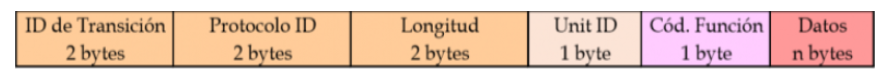
\includegraphics[width=1.0\linewidth]{img/TramaTCP-IP}
	\caption{Estructura de una trama Modbus TCP/IP.}
	\label{fig:tramatcp-ip}
\end{figure}

	\item \textbf{Recibir tramas desde la red mallada y enviarlas hacia una direcci�n externa:} Luego de que se env�a la trama mediante la red WiFi esta tarea espera la respuesta del esclavo al que iba dirigido el mensaje. Cuando la respuesta llega desde la red mallada se utilizan las partes de la trama correspondientes a la longitud para enviar el mensaje mediante el socket TCP/IP hacia el cliente conectado. El tiempo que el mensaje toma en llegar desde el maestro al esclavo correspondiente y de vuelta debe ser menor al tiempo m�ximo de retardo del mensaje que establezca el maestro modbus para que no hayan errores de sincronizaci�n.
	
\end{itemize}

\subsubsection{Nodo serial RS485}

Este tipo de nodo se debe inicializar con los par�metros seriales mediante el modo de configuraci�n en la interfaz gr�fica para el usuario. El c�digo en este nodo fue pensado para que este nodo funcione como una conversi�n de inal�mbrico a serial, puesto que es el encargado de comunicarse con medidores que cumplen la norma RS485 y soportan el protocolo Modbus. Pero tambi�n fue pensado para transformar la trama modbus TCP/IP que llega desde la red mallada en una trama modbus RTU que es la que soportan la mayor�a de medidores con modbus.

\begin{figure}[H]
	\centering
	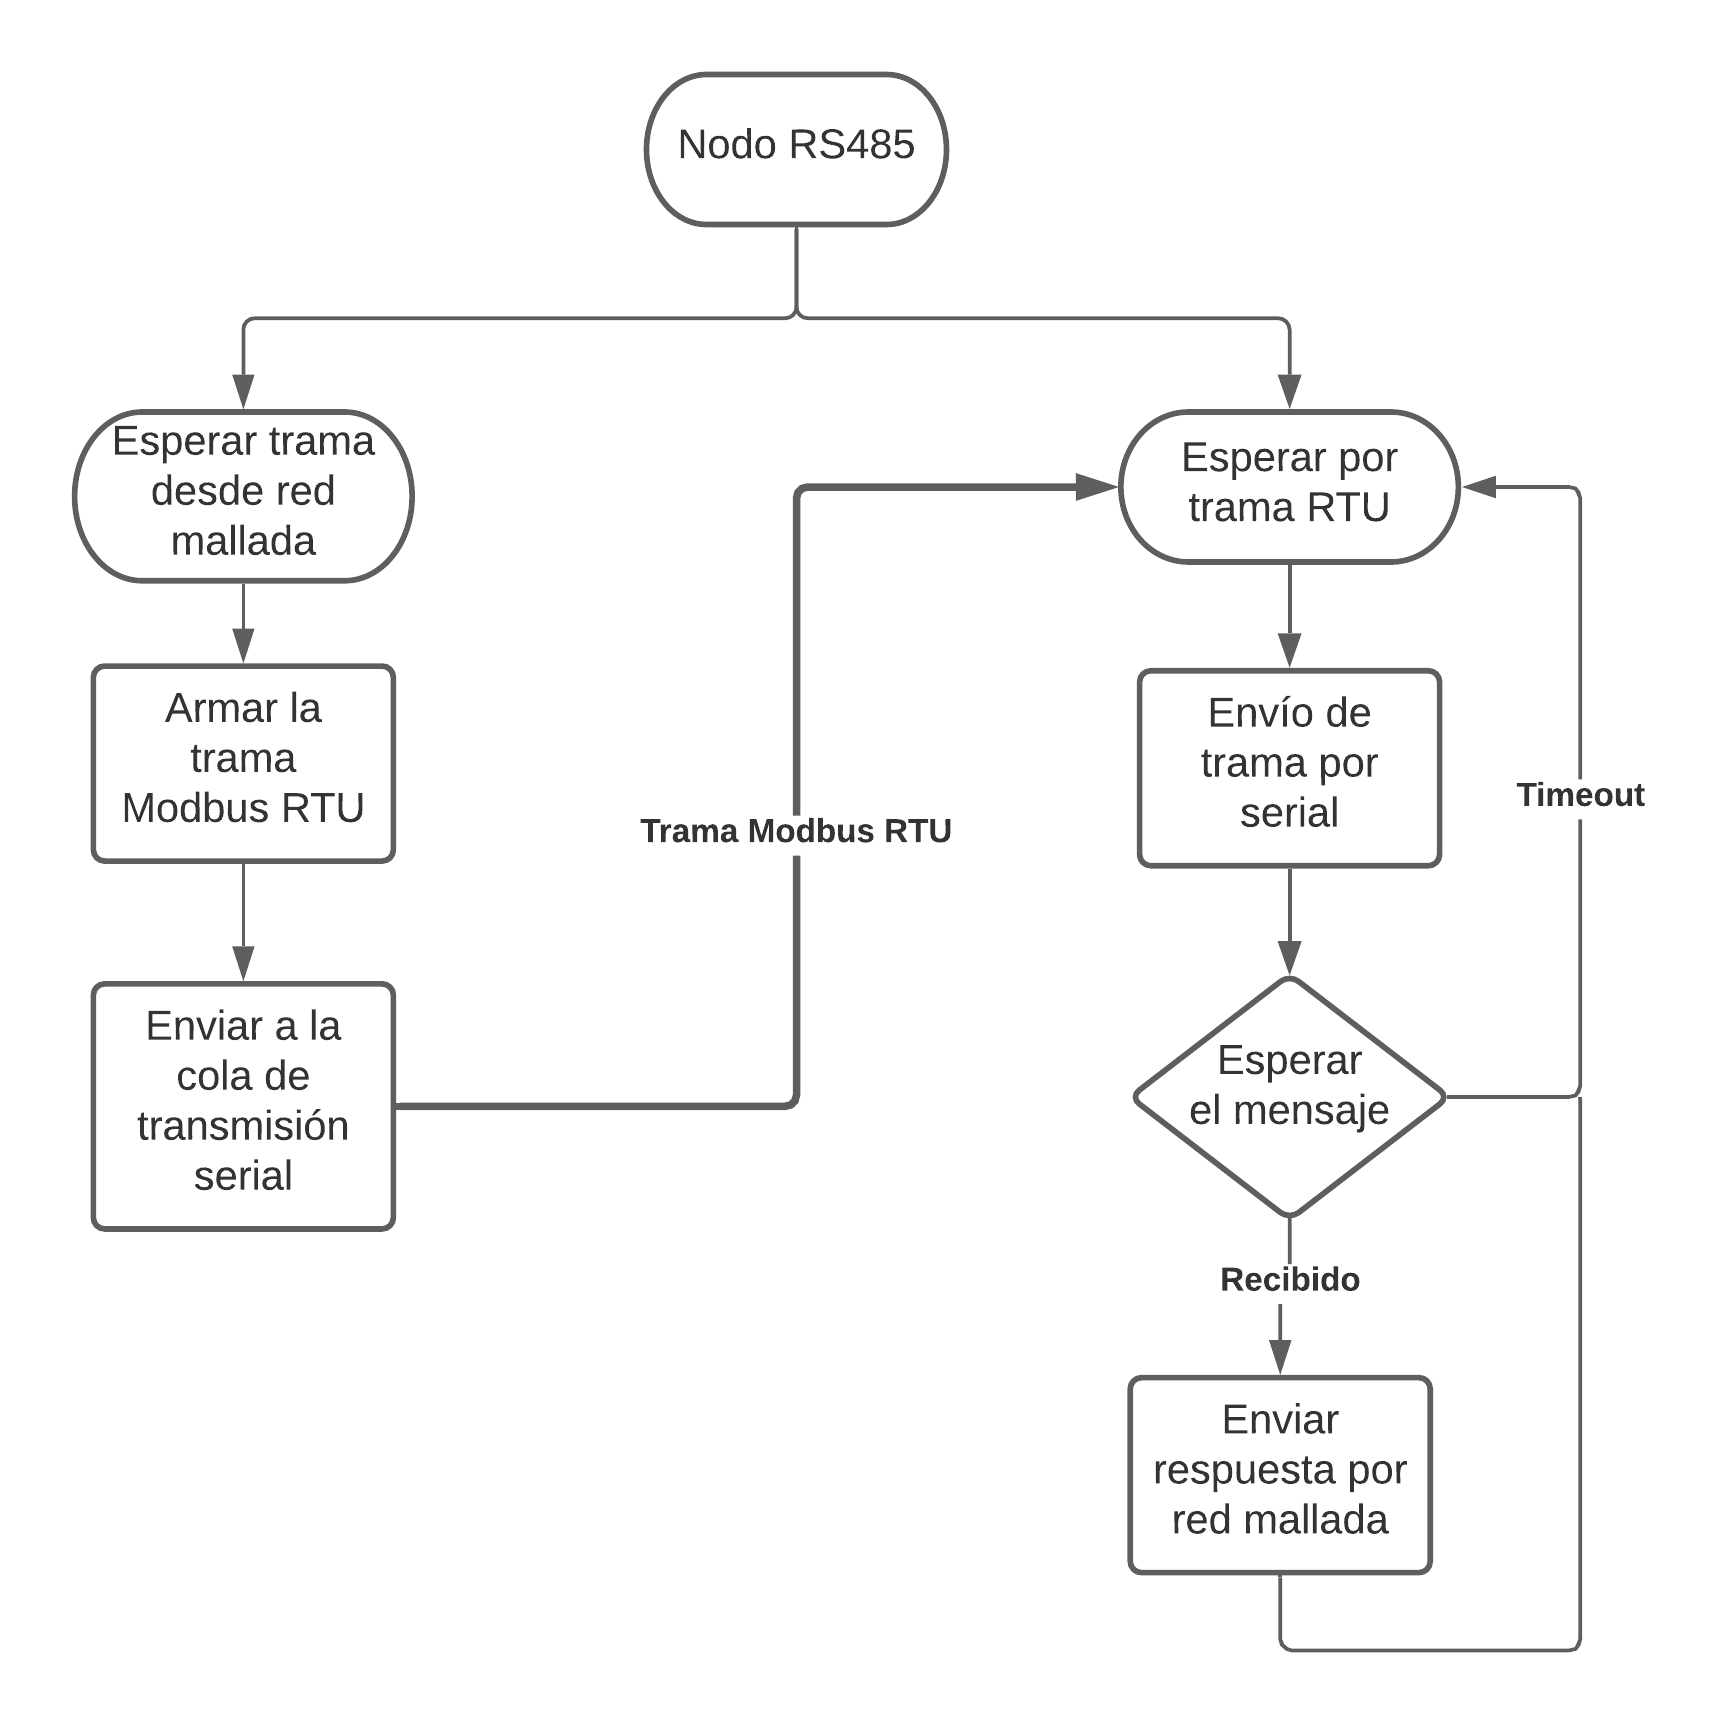
\includegraphics[width=0.8\linewidth]{img/NodoRS485}
	\caption{Diagrama de flujo de las tareas implementadas en el nodo RS485.}
	\label{fig:nodors485}
\end{figure}

\begin{itemize}
	\item \textbf{Esperar la trama desde la red mallada:} Esta tarea se encarga tomar el mensaje que llega y convertir el modbus TCP/IP en un Modbus RTU, esta conversi�n consiste en quitar los 6 primeros bytes de la trama modbus TCP/IP que ser�an los bytes de cabecera y luego colocar una comprobaci�n de errores mediante un CRC de 2 bytes al final de la trama.\\
	
	Una vez realizado este procedimiento, el resultado es puesto en una \textit{cola} del sistema RTOS para comunicarlo hacia la tarea encargada de manejar el bus serial del microcontrolador.\\
	
	\item \textbf{Esperar por trama RTU:} En esta tarea se maneja el bus de datos para la comunicaci�n serial con los medidores. Se toman los datos recibidos en la \textit{cola} del sistema y se env�an mediante el UART del microcontrolador hacia el bus serial con las API del UART que ofrece el fabricante. A partir del env�o comienza a correr un tiempo m�ximo de respuesta que tiene el dispositivo serial conectado al bus para devolver la informaci�n solicitada. \\
	
	Todos los nodos configurados como este tipo de nodo repiten el mensaje independientemente de su contenido pero al ser protocolo modbus solo responder� el esclavo que corresponda con el id contenido en el mensaje. Si la respuesta serial llega, esta se transforma de modbus RTU a modbus TCP/IP para ser enviada al nodo central como respuesta y el nodo queda en espera del siguiente mensaje.
\end{itemize}


\subsubsection{Nodo de entrada por pulsos}

Este nodo se inicializa mediante la interfaz web gr�fica para configuraci�n. Este nodo se cre� con la finalidad de adaptarse a los medidores que se encuentran ya colocados en la mayor�a de conjuntos residenciales y comerciales. Estos medidores poseen una salida binaria que es la que se utiliza para calibrarlos, en esta salida se puede observar un cantidad de impulsos por cada kWh consumido que registra el medidor. \\

La idea de este nodo es tomar esos impulsos y almacenarlos para contar el total de los kWh consumidos, teniendo en consideraci�n la condici�n inicial del medidor y para evitar que la cuenta se pierda por cualquier raz�n este nodo debe almacenar dicho valor en una memoria que sea persistente. \\

Adem�s el nodo debe tener la capacidad de responder a los mensajes enviados por la red mallada y en caso de que dicho mensaje contenga la trama indicada para solicitar el valor de energ�a, responder con dicho registro mediante la red mallada WiFi hacia el nodo central.\\

\begin{figure}[H]
	\centering
	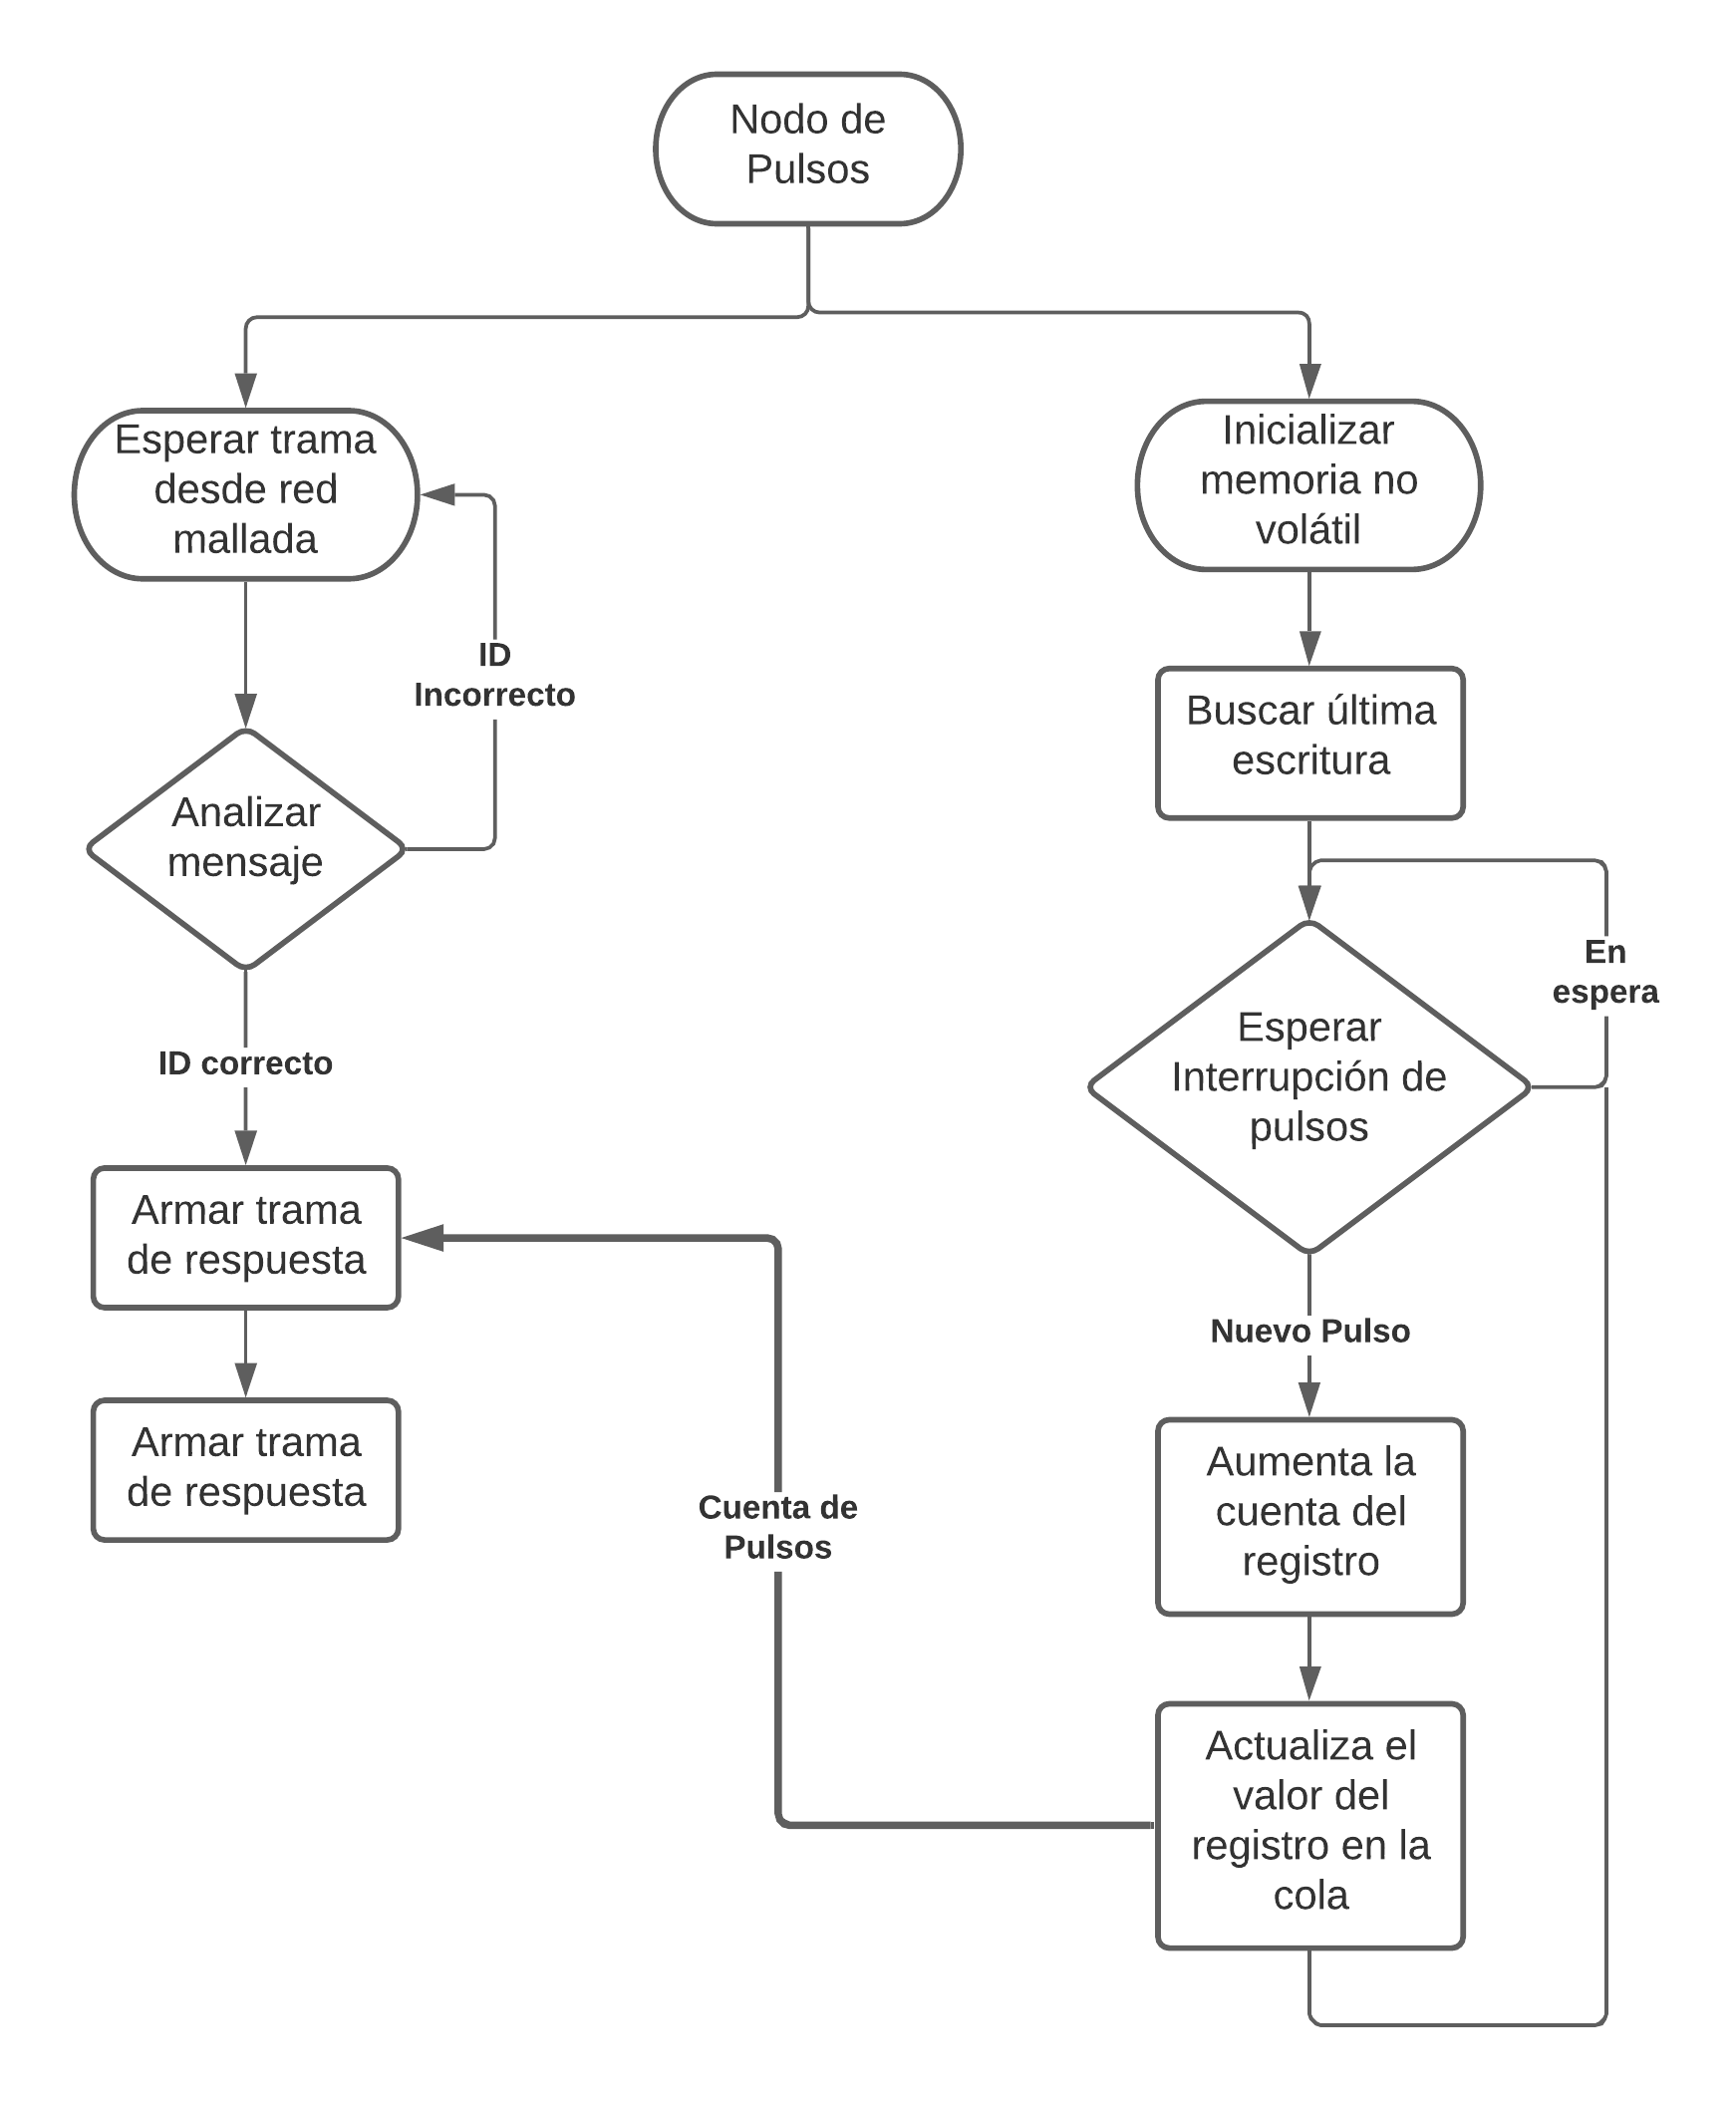
\includegraphics[width=0.8\linewidth]{img/NodoPulsos}
	\caption{Diagrama de flujo de las tareas implementadas en el nodo de pulsos.}
	\label{fig:nodopulsos}
\end{figure}

\begin{itemize}
	\item \textbf{Esperar trama desde la red mallada:} El nodo debe poder comunicarse por la red mallada, por lo que se implement� en este la comunicaci�n mediante la red utilizando la API del fabricante. Esta tarea estar� en espera hasta que llegue el mensaje proveniente de la red mallada, una vez se tenga dicho mensaje se procede a comprobar los campos respectivos al identificador del esclavo, el c�digo de funci�n, el n�mero de registro y el CRC. De comprobarse que todos estos campos son correctos se procede a armar la trama de respuesta con el valor actual de la cuenta de pulsos y se env�a de vuelta al nodo central encapsulado en la trama modbus TCP/IP.\\
	
	\item \textbf{Inicializar memoria no vol�til:} En el microcontrolador utilizado el fabricante utiliza una API llamada NVS (\textit{Non volatile Storage}) para referirse a la memoria flash, esta interfaz de programaci�n ofrece facilidades para tratar y almacenar datos en la memoria flash, as� como la capacidad de manejar las particiones, p�ginas y registros que la comprenden.\\
	
	Para inicializar la memoria no vol�til se utiliza dicha interfaz ofrecida por el fabricante. Cada partici�n de la memoria no vol�til requiere de un nombre, el nombre por defecto es \textit{nvs} pero en este caso ser�n utilizadas varias particiones por lo que se les asign� el nombre de \textit{app1 , app2, app3}. Estos nombres son definidos en la tabla de particiones y ser�n utilizados en el c�digo del programa. \\
	
	\begin{table}[H]
		\centering
		\caption{Tabla de particiones de la aplicaci�n}
		\label{Tab:Partition_table_meters}
		\medskip
		\begin{tabular}{llllll}
			\toprule
			Name & Type & SubType & Offset & Size & Flags\\
			\midrule
			nvs &      data& nvs&    0x9000&  0x6000 & \\
			phyinit& data& phy& 0xf000& 0x1000& \\
			factory&  app&  factory& 0x10000& 1M& \\
			www& data& spiffs& &1M&\\
			app1& data& nvs& &64K&\\
			app2& data& nvs& &64K&\\
			app3& data& nvs& &64K&\\
			\bottomrule
		\end{tabular}
	\end{table}

	\begin{itemize}
		\item \textbf{Tama�os y tablas de particiones}\\
		
		Las p�ginas de partici�n poseen 64kB de la memoria flash cada una, esto debido a que cuando se inicializa una partici�n con el API \textit{NVS} dicha partici�n consume una cantidad de memoria \textit{RAM} proporcional al tama�o de la partici�n inicializada, por lo que para no consumir memoria \textit{RAM} excesiva se escogi� este tama�o de partici�n. \\
		
		La partici�n a su vez se divide en estructuras llamadas p�ginas, que tambi�n poseen nombres, estas p�ginas tienen un tama�o de 4kB (por defecto) y el nombre por defecto de la p�gina inicial es \textit{storage}, el resto de las 15 p�ginas fueron nombradas con los nombres \textit{pv0 - pv14}.\\
		
		Y las p�ginas est�n compuestas por registros, 126 para ser exactos, llamados por el fabricante como entradas. Estas llevan tambi�n un nombre y fueron asignadas como (\textit{e0-e125}). Las entradas son capaces de almacenar diferentes tipos de datos: enteros con y sin signo, cadenas de caracteres y arreglos.\\
		
		Es importante que se consideren los l�mites f�sicos de la memoria flash, un mismo espacio de memoria puede sobreescribirse hasta unas 100000 veces antes de da�arse. Por lo que la cantidad de veces que se reescribe en una entrada en el algoritmo se fij� como 50000, para preservar el estado f�sico de la memoria. Para el algoritmo, una entrada se encuentra llena cuando alcanza ese n�mero de veces escrita.\\
		
		\item \textbf{Buscar la �ltima escritura en la memoria}\\
		
		El algoritmo para almacenar los pulsos comienza en la partici�n \textit{app1} y comprueba si esta partici�n se encuentra 'llena' mediante una bandera l�gica en la pagina principal \textit{storage}, de ser as� cierra la partici�n actual y busca en la siguiente hasta encontrar una que no est� llena, de no encontrar una disponible se emite una alerta mediante el serial.\\
		
		Una vez en la partici�n se busca la �ltima p�gina en la que se escribi� mediante un entero almacenado en la p�gina principal \textit{storage}. En la �ltima p�gina escrita se cuenta la cantidad de entradas escritas, con este numero se puede saber la �ltima entrada que se escribi�. \\
		
		Se toma el valor de esa �ltima entrada y se le suman todas las entradas, p�ginas y particiones anteriores adem�s de la condici�n inicial de kWh para saber la cantidad de pulsos que se llevan en la cuenta y se almacena en el registro para estar disponible en caso de que se deba enviar mediante la red WiFi.\\
		
		\item \textbf{Nuevo pulso detectado}\\
		
		Por �ltimo cuando se produce un nuevo pulso y se detecta mediante una interrupci�n en el pin asignado, el programa aumenta la cuenta de pulsos total que se encuentra en el registro para enviar por la red y tambi�n aumenta la cuenta en la entrada actual para que la informaci�n sea persistente.\\
		
		En caso de llenarse una entrada se cambia a la siguiente hasta llegar a la entrada \textit{e125}, luego se cambia a la siguiente p�gina y se modifica el entero correspondiente a la �ltima p�gina escrita en \textit{storage}, hasta llegar a la p�gina \textit{pv14}, en este caso se coloca una bandera l�gica en la p�gina \textit{storage} para avisar que se encuentra llena la partici�n y se cambia a la siguiente. Luego vuelve al estado de espera de la siguiente interrupci�n por pulsos.
	\end{itemize}

\item \textbf{C�lculos de vida �til estimada seg�n el uso de la memoria flash}\\

Tomando la como referencia el medidor de una casa promedio en Espa�a, al a�o se alcanza la cifra de 9922 kWh consumidos por lo que haciendo una estimaci�n para la duraci�n de la memoria tendr�amos:

\begin{equation}
	52\; \frac{semana}{anio} \times 7\; \frac{dia}{semana} \times 24\; \frac{horas}{dia} = 8736\; \frac{horas}{anio}
\end{equation}


\begin{equation}
	\dfrac{9922\; \frac{kWh}{anio}}{8736\; \frac{horas}{anio}} = 1,1358\;\frac{kWh}{hora}
\end{equation}

La cantidad de pulsos emitidos por kWh depende enteramente del medidor, puesto que todos tienen valores diferentes. Para un medidor de 1800 $\frac{imp}{kWh}$ que es el que se utiliza para las pruebas de sistema, se tiene que:

\begin{equation}
	1,1358\; \frac{kWh}{hora} \times 1800\; \frac{impulsos}{kWh} = 2045\; \frac{impulsos}{hora}
\end{equation}

En el c�lculo de la vida �til es necesario tomar en cuenta la cantidad de impulsos que se puede almacenar en las particiones:

\begin{equation}
	126\; entradas \times 15\; paginas \times 50k \frac{impulsos}{entrada} = 94,5\; Mimpulsos
\end{equation}
\begin{equation}
	94,5\; Mimpulsos \times 2045\; \frac{impulsos}{hora} = 46210\; horas\; o\; 5\; anios
\end{equation}\\


Esto significa que cada partici�n durar�a para el consumo de una casa promedio 5 a�os, al tener 3 particiones inicialmente se estar�an garantizando seg�n los c�lculos unos 15 a�os de vida �til.\\

Esto sin considerar que el n�mero de particiones de 64kB se puede aumentar y solo se ve limitado por el tama�o de la memoria flash del micro que en muchos casos llega a ser entre 2 y 16 MB.

\end{itemize}

\subsubsection{Nodo Repetidor}

El nodo repetidor es un nodo que ha sido configurado para ser parte de la red mallada sin tener conexiones f�sicas con alguna remota mediante un bus serial o con un medidor de energ�a mediante su salida de calibraci�n.\\

Este tipo de nodos es �til para ampliar la cobertura de la red en caso de que sea necesario abarcar un espacio o tener mayor densidad de nodos en una zona espec�fica. Este nodo no posee tareas implementadas en sus n�cleos, solo posee el c�digo necesario para ser parte de la red y repetir en ambos sentidos los mensajes que lleguen a este.\\


\subsubsection{Otras consideraciones}

Las tareas se crean en lineas de c�digo contiguas de modo tal que no hay un orden de creaci�n de ellas, pues el objetivo es que estas se ejecutan en paralelo y el RTOS sea el encargado de esperar por los datos necesarios para su ejecuci�n sincronizada y correcta.\\


%==================================================================
\chapter{PRUEBAS Y RESULTADOS}\label{CAP:exp}
%\markboth{Tu Segundo Cap?tulo}{Tu Segundo Cap?tulo}%
%% !TeX spellcheck = es_ES
% !TeX encoding = ISO-8859-1

Una vez establecido el hardware y realizado el dise�o del software necesario para implementar la aplicaci�n en el microcontrolador se realiz� una serie de pruebas para constatar la correcta implementaci�n del sistema.

\section{Resultados de la interfaz gr�fica}

Para realizar las pruebas del sistema que se presentan a continuaci�n se debi� configurar cada uno de los nodos utilizando la interfaz gr�fica implementada en el modo de configuraci�n. A continuaci�n se ilustra el procedimiento y las distintas pantallas implementadas en ello:

\begin{figure}[H]
	\centering
	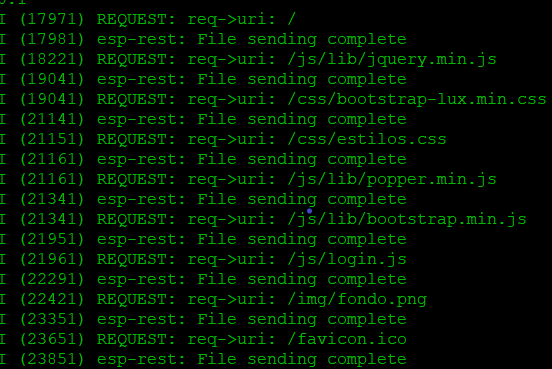
\includegraphics[width=0.6\linewidth]{img/ejemploPagina}
	\caption{Log serial del microcontrolador en modo servidor HTTP cuando es enviada una de las pantallas.}
	\label{fig:ejemplopagina}
\end{figure}

Cuando el usuario solicita cualquier p�gina al servidor se produce recibe la petici�n y se procesa enviando posteriormente el archivo solicitado como se puede ver en la figura \ref{fig:ejemplopagina}, esto es com�n para todas las pantallas y se puede ver afectado por la congesti�n de la red local, ya que el env�o se realiza mediante de esta.\\

\begin{figure}[H]
	\centering
	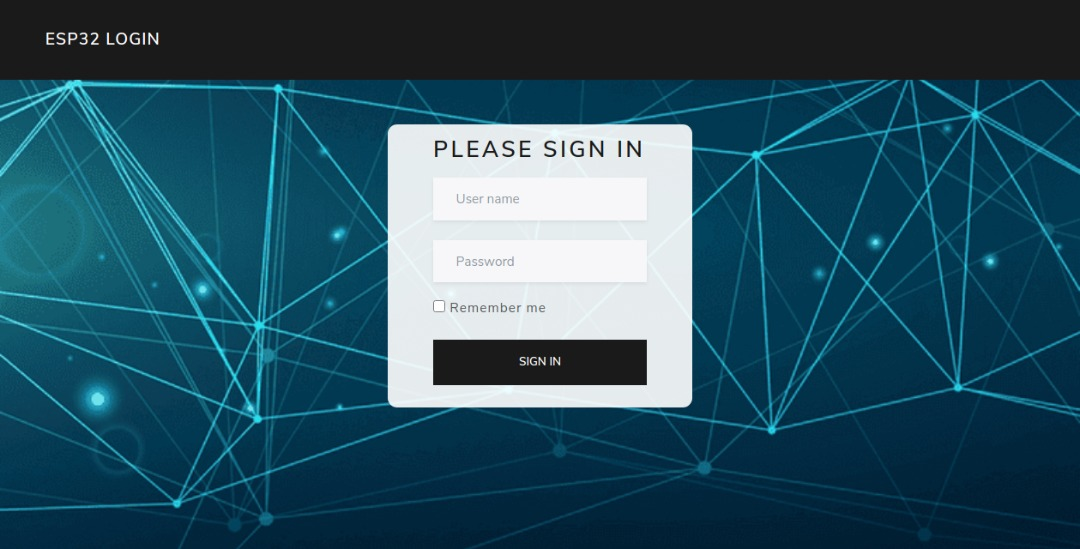
\includegraphics[width=0.9\linewidth]{img/Login}
	\caption{Vista de la pantalla de inicio de sesi�n del usuario.}
	\label{fig:login}
\end{figure}

Seguidamente, se puede observar la pantalla de inicio de sesi�n, figura \ref{fig:login}, en la que el usuario debe introducir de manera correcta clave y contrase�a para acceder a la configuraci�n del equipo, considerando la seguridad del mismo.\\

\begin{figure}[H]
	\centering
	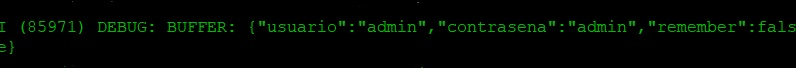
\includegraphics[width=1\linewidth]{img/loginJSONv2}
	\caption{Mensaje recibido en el servidor cuando el usuario rellena el inicio de sesi�n y env�a los datos.}
	\label{fig:loginjson}
\end{figure}

Una vez es iniciada la sesi�n se muestra el formulario de configuraci�n de la red mallada, en el que se introducen los par�metros de configuraci�n de dicha red.

\begin{figure}[H]
	\centering
	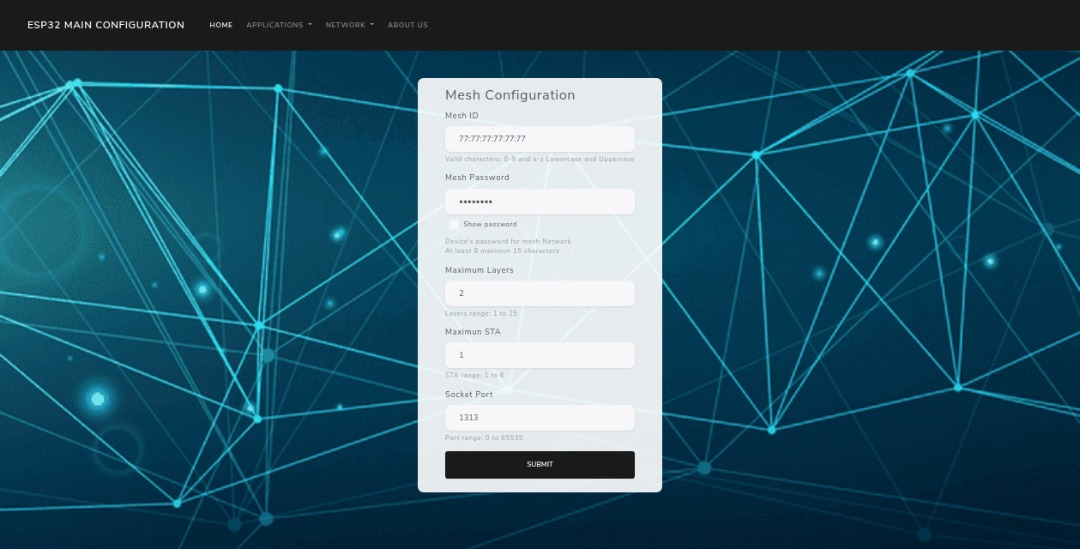
\includegraphics[width=0.9\linewidth]{img/FormMesh}
	\caption{Vista de la pantalla del formulario de par�metros de la red mallada.}
	\label{fig:formmesh}
\end{figure}

\begin{figure}[H]
	\centering
	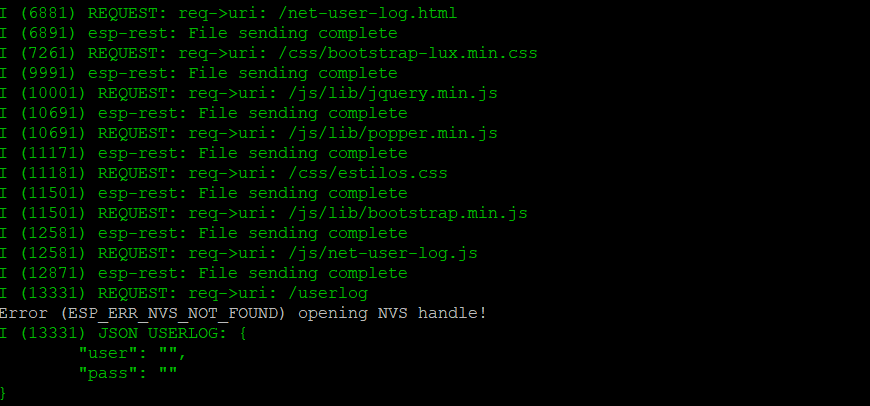
\includegraphics[width=1\linewidth]{img/meshJSON}
	\caption{Mensaje recibido en el servidor cuando el usuario rellena el formulario de red mallada y env�a los datos.}
	\label{fig:meshjson}
\end{figure}


Con los par�metros en las figuras \ref{fig:formmesh} y \ref{fig:meshjson} se puede inicializar la red mallada. Se procede luego mediante el men� de la barra superior de la p�gina para acceder al formulario de par�metros seriales.

\begin{figure}[H]
	\centering
	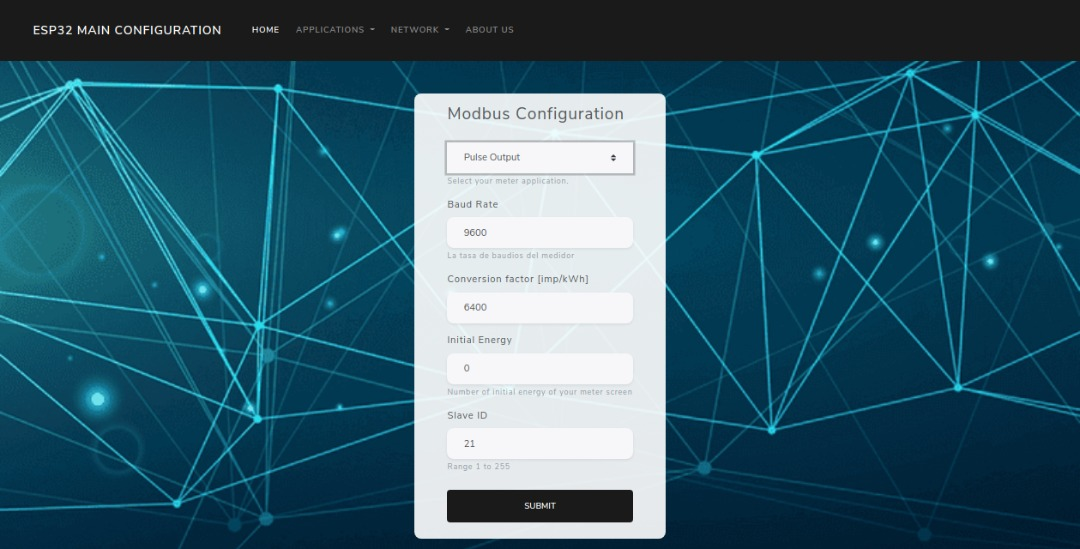
\includegraphics[width=0.9\linewidth]{img/FormModbus}
	\caption{Vista de la pantalla de formulario de par�metros seriales.}
	\label{fig:formmodbus}
\end{figure}

\begin{figure}[H]
	\centering
	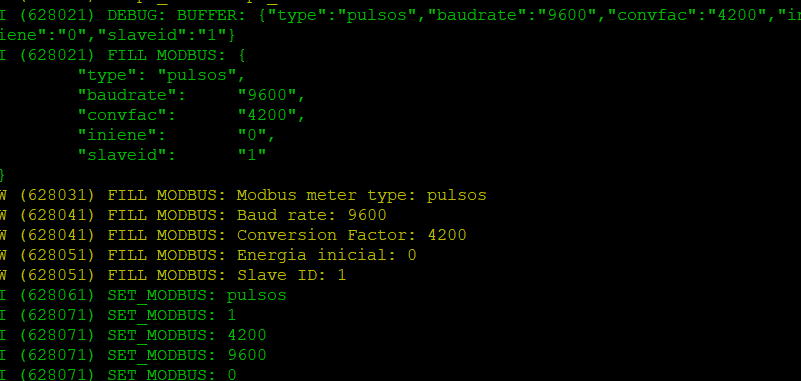
\includegraphics[width=1\linewidth]{img/modbusJSON}
	\caption{Mensaje recibido en el servidor cuando el usuario rellena el formulario de par�metros seriales y env�a los datos.}
	\label{fig:modbusjson}
\end{figure}

 Los par�metros de las figuras \ref{fig:formmodbus} y \ref{fig:modbusjson} son los par�metros requeridos para para la extracci�n de la data desde el medidor. En la siguiente pantalla se debe rellenar el formulario de la red local:

\begin{figure}[H]
	\centering
	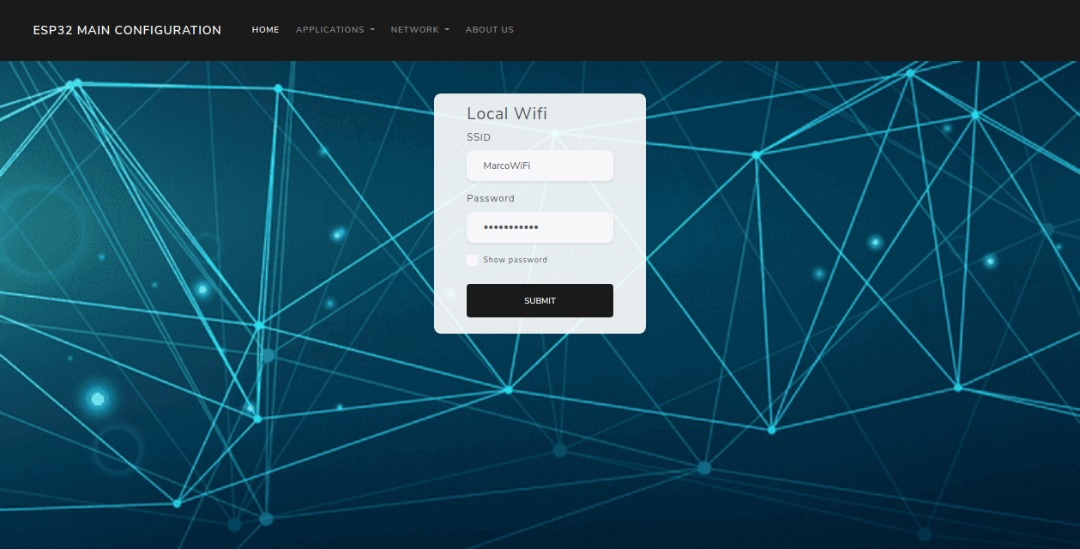
\includegraphics[width=0.9\linewidth]{img/LocWifijpg}
	\caption{Vista de la pantalla de par�metros de red local}
	\label{fig:locwifijpg}
\end{figure}

\begin{figure}[H]
	\centering
	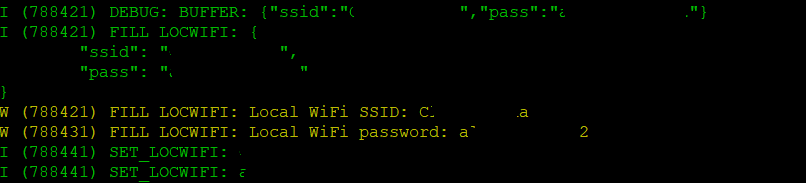
\includegraphics[width=1\linewidth]{img/locwifiJSON}
	\caption{Mensaje recibido en el servidor cuando el usuario rellena el formulario de red local y env�a los datos.}
	\label{fig:locwifijson}
\end{figure}

Los par�metros de las figuras \ref{fig:locwifijpg} y \ref{fig:locwifijson} son utilizados para que el equipo pueda tener acceso al WiFi en caso de ser el nodo central. Con este paso se cumple el m�nimo necesario para que el equipo funcione. Por �ltimo se realiz� una pantalla para cambiar el usuario y la contrase�a de inicio de sesi�n, en caso de que se quiera modificar esta.

\begin{figure}[H]
	\centering
	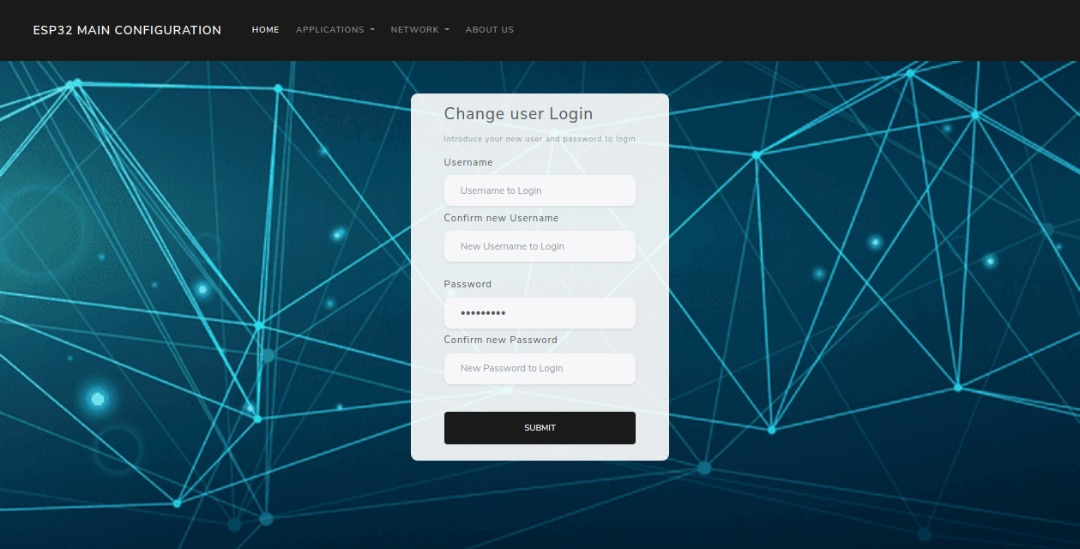
\includegraphics[width=0.9\linewidth]{img/UserLog}
	\caption{Vista de la pantalla para modificar los par�metros de acceso del usuario.}
	\label{fig:userlog}
\end{figure}

\begin{figure}[H]
	\centering
	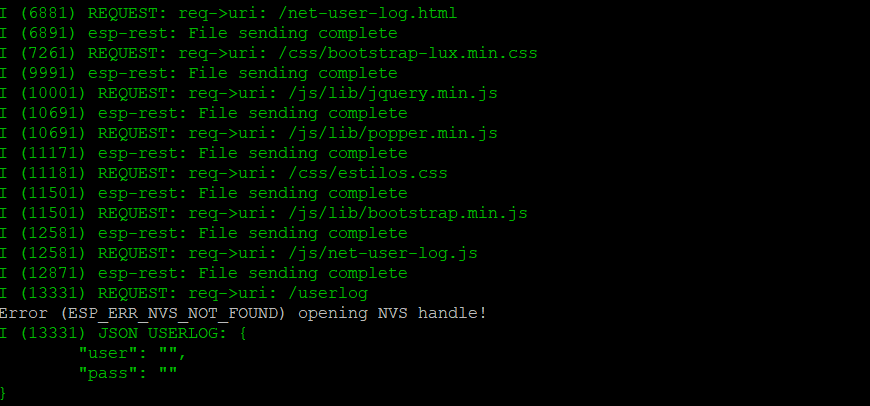
\includegraphics[width=0.7\linewidth]{img/userJSON}
	\caption{Mensaje recibido en el servidor cuando el usuario rellena el formulario de actualizar usuario y contrase�a y env�a los datos.}
	\label{fig:userjson}
\end{figure}


\section{Prueba de funcionamiento del sistema}

Una vez introducidos los datos de configuraci�n en el modo anterior, se reinician los nodos para que la red comience a funcionar. Cada nodo se conecta al WiFi y entre s�, luego se realiza una votaci�n en la que se elige un nodo central, estableci�ndose as� la primer capa de la red.\\

Posteriormente se establece la estructura de la red, en el caso de estas pruebas realizadas se coloc� en los par�metros del nodo central un m�ximo de tres (3) capas de profundidad para la red y un  m�ximo de dos (2) conexiones con nodos hijos para dicho nodo central.\\

En la siguiente capa de la red, la segunda capa, se encuentra un nodo repetidor que funcionar� como demostraci�n de la capacidad de la red de comunicarse con nodos en capas m�s profundas a trav�s de otros nodos. El mismo fue configurado con la capacidad de tener para esta prueba un (1) solo nodo hijo conectado. En esta segunda capa tambi�n se encuentra uno de los nodos a medir, el nodo de pulsos, conectado directamente con el nodo central.\\

En la tercera y �ltima capa para esta prueba y conectado al nodo enlace se encuentra el nodo de transmisi�n serial RS485. Un diagrama de la prueba quedar�a de la siguiente manera:

\begin{figure}[H]
	\centering
	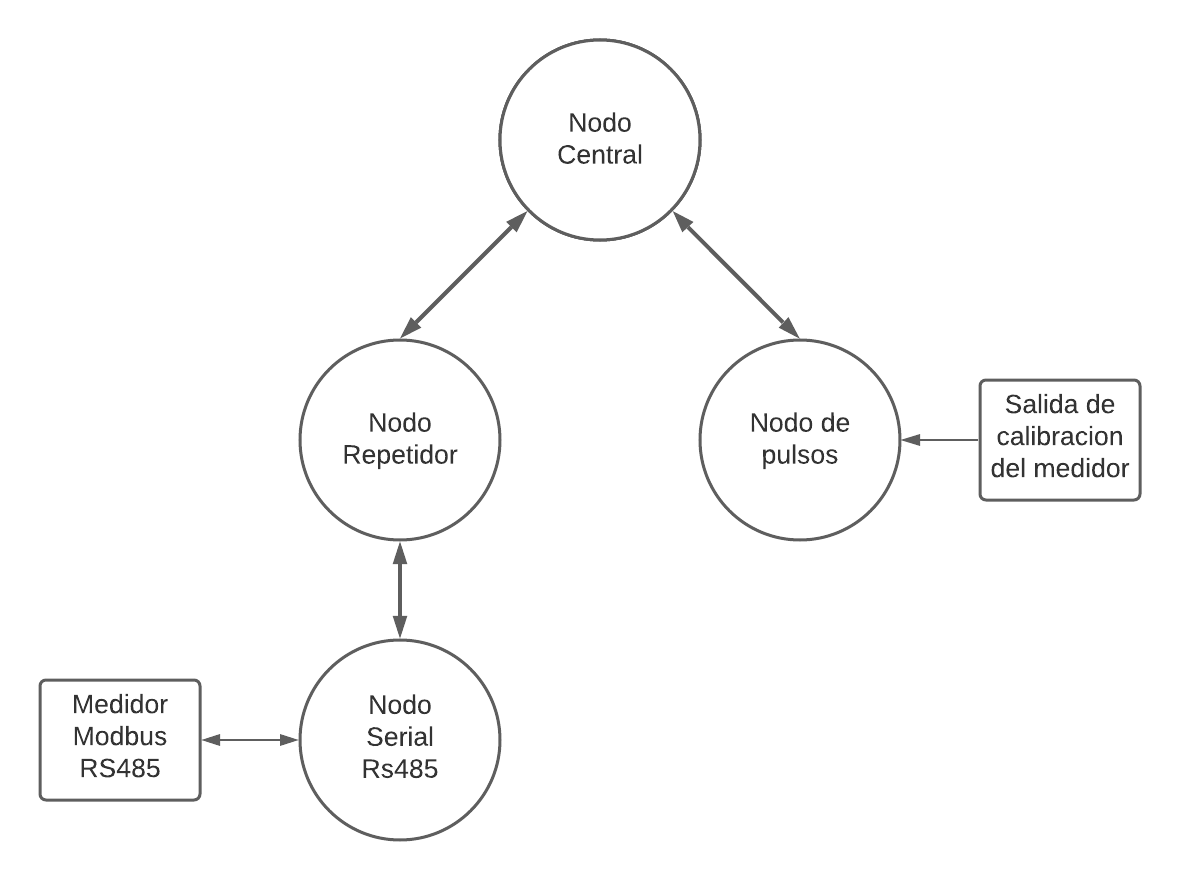
\includegraphics[width=0.7\linewidth]{img/DiagramaPrueba}
	\caption{Diagrama general de la red para pruebas.}
	\label{fig:diagramaprueba}
\end{figure}

En esta red se realizaran pruebas de extracci�n de datos para comprobar el funcionamiento de los nodos y pruebas de restablecimiento del sistema en caso de que los nodos se desconecten de la red.\\

El tiempo entre env�o de mensajes en la red se estableci� en 1 segundo y el m�ximo tiempo de respuesta aceptado se estableci� en 5s para las siguientes pruebas.
 
\subsection{Extracci�n de datos del nodo contador de pulsos}

\begin{table}[H]
	\centering
	\caption{Registro de mensajes del maestro sobre la comunicaci�n con el esclavo de pulsos.}
	\label{Tab:Master2Pulse}
	\medskip
	\begin{tabular}{l|lllrr}
		\toprule
		\multicolumn{6}{c}{Registro del maestro modbus} \\
		Prueba N\textdegree&Enviados& Recibidos& Tiempo [s]& Errores & Error[\%]\\
		\midrule
		1&1500  & 1499  & 2223,801 & 13 & 0,87\\
		2&1500 & 1499  & 2226,643 & 16 & 1,07\\
		3&1500& 1500 & 2226,970 & 15 & 1\\
		\bottomrule
	\end{tabular}
\end{table}

\begin{table}[H]
	\centering
	\caption{Registro de mensajes del nodo contador de pulsos sobre la comunicaci�n con el maestro.}
	\label{Tab:Pulse2Master}
	\medskip
	\begin{tabular}{l|lllrr}
		\toprule
		\multicolumn{6}{c}{Nodo contador de pulsos} \\
		 Prueba N\textdegree& Recibidos & Enviados & Tiempo [s] & Error de procesamiento & Error[\%]\\
		\midrule
		1&1499 & 1499&2223,801 & - & -\\	
		2&1499 & 1499&2226,643 & - & -\\
		3&1500 & 1500&2226,970 & - & -\\
		\bottomrule
	\end{tabular}
\end{table}

El nodo contador de pulsos culmin� con una cantidad de errores m�xima en todas las pruebas realizadas del 1,07\% en el registro del maestro modbus (tabla \ref{Tab:Master2Pulse}), lo que denota el correcto funcionamiento de la red con este nodo. \\

Se observa en la tabla \ref{Tab:Pulse2Master} que la cantidad de mensajes recibidos y enviados es la misma por lo que no hubo errores en el procesamiento del nodo, esta cantidad adem�s coincide casi en totalidad con el registro del maestro por lo que se infiere que los errores registrados son errores debido al timeout � error de identificador en la trama enviada por el nodo.

\subsection{Extracci�n de datos del nodo RS485}


\begin{table}[H]
	\centering
	\caption{Registro de mensajes del maestro sobre la comunicaci�n con el nodo serial rs485.}
	\label{Tab:Master2Serial}
	\medskip
	\begin{tabular}{l|lllrr}
		\toprule
		\multicolumn{6}{c}{Registro del maestro modbus} \\
		Prueba N\textdegree&Enviados& Recibidos& Tiempo[s]& Errores& Error[\%]\\
		\midrule
		1&1500   & 1481  & 2761,411 & 67 & 4,46 \\
		2&1500  & 1481  & 2761,803 & 67 & 4,46 \\
		3&1500 & 1480 & 2758,267 & 65 & 4,33\\
		\bottomrule
	\end{tabular}
\end{table}

\begin{table}[H]
	\centering
	\caption{Registro de mensajes del nodo serial rs485 sobre la comunicaci�n con el maestro.}
	\label{Tab:Serial2Master}
	\medskip
	\begin{tabular}{l|lllrr}
		\toprule
		\multicolumn{6}{c}{Nodo serial RS485} \\
		Prueba N\textdegree & Recibidos & Enviados & Tiempo[s] & Error de procesamiento & Error[\%]\\
		\midrule
		1&1498  & 1481 &2761,411 & 17 & 1,13\\	
		2&1498  & 1481 &2761,803 & 17 & 1,13\\
		3&1498 & 1480 &2758,267 & 18 & 1,20 \\
		\bottomrule
	\end{tabular}
\end{table}

La diferencia en la cantidad de mensajes enviados y recibidos evidencia perdidas de paquetes en la red y un funcionamiento menor que el nodo de pulsos, las tasas de error registradas por el maestro denotan un porcentaje m�ximo de 4,46\% como se observa en la tabla \ref{Tab:Master2Serial}.\\

Con los datos de la tabla \ref{Tab:Serial2Master} se puede observar que hubo un m�ximo de 18 errores en el procesamiento de los mensajes en una prueba, estos errores en el procesamiento del nodo pueden surgir debido al tiempo de espera m�ximo que se tiene programado en el bus serial de este tipo de nodos, puede deberse al tiempo de respuesta del medidor asociado al nodo que puede verse saturado y responder menos mensajes de los que se demandan.

\section{Prueba de restablecimiento del sistema}
\subsection{Para el nodo central}

\begin{figure}[H]
	\centering
	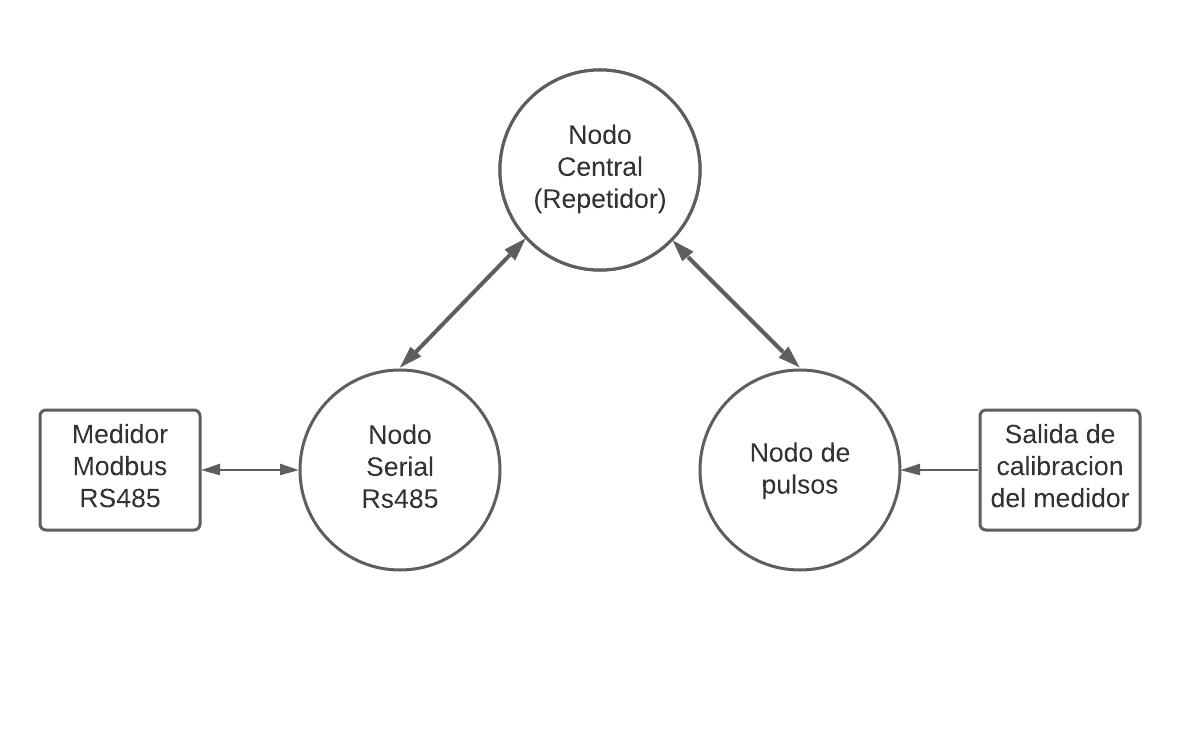
\includegraphics[width=0.7\linewidth]{img/ReestablecerRoot}
	\caption{Ejemplo de la red restablecida luego de desconectar el nodo central si el nodo repetidor gana la votaci�n.}
	\label{fig:reestablecerroot}
\end{figure}


\begin{table}[H]
	\centering
	\caption{Tiempo de recuperaci�n de la red cuando es desconectado el nodo central.}
	\label{Tab:healingMasterNode}
	\medskip
	\begin{tabular}{lr}
		\toprule
		Prueba N\textdegree & Tiempo de recuperaci�n [ms] \\
		\midrule
		1&25541 \\
		2&24598 \\
		3&25720 \\
		4&25231 \\
		5&24896 \\
		\bottomrule
	\end{tabular}
\end{table}

De las pruebas y el tiempo en la tabla \ref{Tab:healingMasterNode} se puede observar que el nodo central como nodo fundamental de la red tarda m�s de 25 segundos en recuperarse, a este tiempo le afectan varios factores: El tiempo que toma en darse cuenta la red que se perdi� la conexi�n con dicho nodo central, luego el tiempo de votaci�n para la elecci�n del nuevo nodo central y por �ltimo el tiempo de reordenamiento de la red (puede verse afectado por la cantidad de nodos).\\

Al ser solo 3 nodos los restantes y tardar dicha cantidad de tiempo, este es un factor a considerar para su uso en aplicaciones cr�ticas. 


\subsection{Para cualquier otro nodo}

\begin{figure}[H]
	\centering
	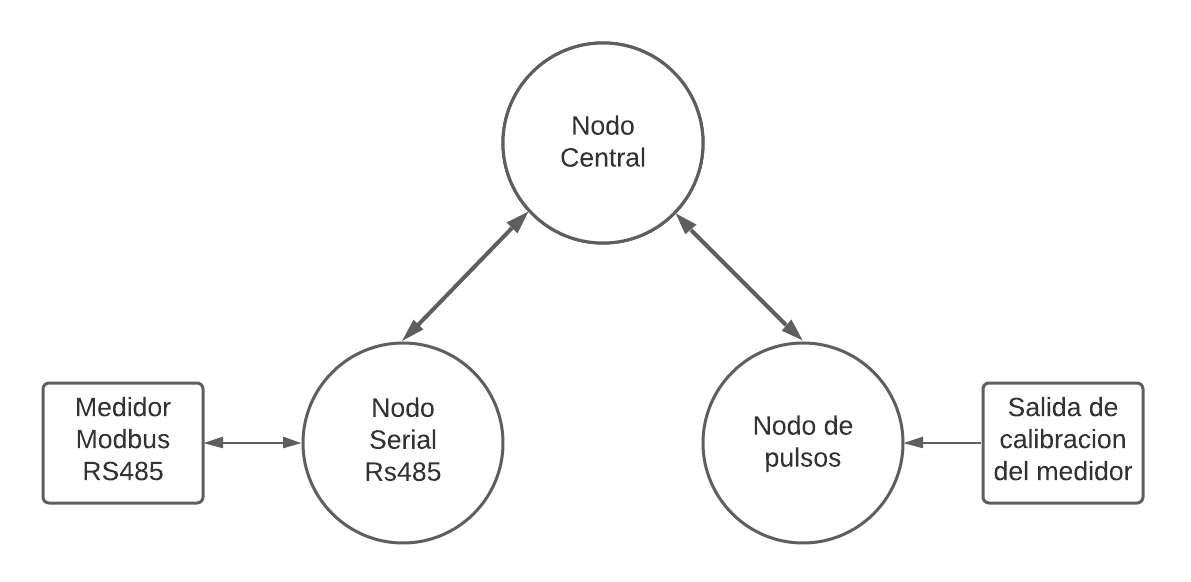
\includegraphics[width=0.7\linewidth]{img/ReestablecerOtro}
	\caption{Ejemplo de la red restablecida luego de desconectar el nodo repetidor.}
	\label{fig:reestablecerotro}
\end{figure}


\begin{table}[H]
	\centering
	\caption{Tiempo de recuperaci�n de la red cuando es desconectado un nodo, exceptuando el nodo central.}
	\label{Tab:healingAnyNode}
	\medskip
	\begin{tabular}{lr}
		\toprule
		Prueba N\textdegree & Tiempo de recuperaci�n [ms] \\
		\midrule
		1&17776 \\
		2&18163 \\
		3&17142 \\
		4&17964 \\
		5&18162 \\
		6&18254 \\
		7&18422 \\
		8&17968 \\
		9&17566 \\
		10&17001 \\
		\bottomrule
	\end{tabular}
\end{table}

En este caso (tabla \ref{Tab:healingAnyNode}) se observa que el tiempo es varios segundos menor respecto al tardado para el restablecimiento del nodo central, para un nodo cualquiera no se debe realizar una votaci�n ni el restablecimiento de la totalidad de la red sino que puede ser parcialmente renovada, reduciendo as� el tiempo que se tarda la red en sanar la p�rdida.

%==================================================================
\chapter{CONCLUSIONES}\label{CAP:conclu}
%\markboth{Tu Segundo Cap?tulo}{Tu Segundo Cap?tulo}%
%% !TeX encoding = ISO-8859-1
% !TeX spellcheck = es_ES

\begin{itemize}
	\item
	\item
	\item
	\item
	\item
\end{itemize}

%==================================================================
\chapter{RECOMENDACIONES}\label{CAP:recomend}
%\markboth{Tu Segundo Cap?tulo}{Tu Segundo Cap?tulo}%
%% !TeX spellcheck = es_ES
% !TeX encoding = ISO-8859-1

\begin{itemize}
	\item
	\item
	\item
	\item
	\item
\end{itemize}

\appendix

\renewcommand \thechapter{\Roman{chapter}}
%==================================================================
\chapter{T�TULO DEL ANEXO}\label{CAP:anexo0}
%\markboth{Tu anexo}{Tu anexo}%
%\input{apendice0.tex}%

%==================================================================
\chapter{T�TULO DEL ANEXO}\label{CAP:anexo1}
%\markboth{Tu anexo}{Tu anexo}%
%\input{apendice1.tex}%

%\backmatter
%==================================================================
\chapter{T�TULO DEL ANEXO}\label{CAP:anexo2}
%\markboth{Tu anexo}{Tu anexo}%
%\input{apendice2.tex}%



%\backmatter

%==================================================================
\newpage
%\markboth{Referencias}{Referencias}%
%\addcontentsline{toc}{chapter}{Referencias}%

% References here (outcomment the appropriate case)
% CASE 1: BiBTeX used to constantly update the references (while the paper is being written).
\bibliographystyle{IEEEtran}%%% outcomment this and next line in Case 1 siam
%\bibliographystyle{apalike}%
\renewcommand{\bibname}{REFERENCIAS}
\let\oldbibsection\bibsection
\bibliography{MRTG} % if more than one, comma separated and without extension bib


% CASE 2: BiBTeX used to generate EIETdeG.bbl (to be further fine tuned)
%% !TeX spellcheck = es_ES
% !TeX encoding = ISO-8859-1

\documentclass[letterpaper,titlepage,12pt,oneside,spanish,final]{report_eie}

%\documentclass[letterpaper,titlepage,12pt,twoside,openright,spanish,final]{report_eie}

%%%%%%%%%%%%%%%%%%%%%%%%%%%%%%%%%%%%%%%%%%%%%%%%%%%%%%%%%%%%%%%%%%%%%%%%
\usepackage[spanish]{babel}
%\usepackage[latin1]{inputenc}
\usepackage[utf8]{inputenc} %Reconoce tildes y otros simbolos propios del espa?ol
\usepackage[T1]{fontenc}  %Estilo de fuente time new roman

\usepackage{amssymb}
\usepackage{amsfonts}
\usepackage{amsmath}
\usepackage{latexsym}
\usepackage[letterpaper]{geometry}

\usepackage{float}
\usepackage{makeidx}
\usepackage{color}

\usepackage{tocbibind}
\usepackage{acronym}
\usepackage{caption2}
\usepackage{epsfig}
\usepackage{graphicx}
\usepackage{slashbox}
\usepackage{setspace}
\usepackage{multicol}
\usepackage{longtable}
%\usepackage{doublespace}

\usepackage{fancyhdr}
%\usepackage{fancyheadings}

\usepackage{booktabs}



%========= Define el estilo de referencias ===============
%\usepackage[round,authoryear]{natbib}%\usepackage[square,numbers]{natbib}%
%\usepackage[comma,authoryear]{natbib} esto est? abajo

%========= Define el estilo de referencias APA ===============
%\usepackage[natbibapa]{apacite}%natbibapa
\usepackage[numbers]{natbib}%natbibapa
%\usepackage[apaciteclassic]{apacite}%natbibapa
%\usepackage[compact]{titlesec} %modificar espaciado


\usepackage{url}
%\usepackage{hyperref}
\usepackage[colorlinks=true,urlcolor=black,citecolor=black,anchorcolor=black,linkcolor=black]{hyperref}

\UseRawInputEncoding

%%%%%%%%%%%%%%%%%%%%%%%%%%%%%%%%%%%%%%%%%%%%%%%%%%%%%%%%%%%%%%%%%%
%            Definici?n del Documento PDF, (PDFLaTeX)            %
%%%%%%%%%%%%%%%%%%%%%%%%%%%%%%%%%%%%%%%%%%%%%%%%%%%%%%%%%%%%%%%%%%

\hypersetup{pdfauthor=Nombre}

\hypersetup{pdftitle=T�tulo}%

\hypersetup{pdfkeywords=Palabras clave}

\pdfstringdef{\Produce}{Escuela de Ingenier�a El�ctrica, Facultad de Ingenier�a, UCV}%

\pdfstringdef{\area}{�rea del trabajo}

\hypersetup{pdfproducer=\Produce}

\hypersetup{pdfsubject=\area}

\hypersetup{bookmarksnumbered=true}

%%%%%%%%%%%%%%%%%%%%%%%%%%%%%%%%%%%%%%%%%%%%%%%%%%%%%%%%%%%%%%%%%%

%%%%%%%%%%%%%%%%%%%%%%%%%%%%%%%%%%%%%%%%%%%%%%%%%%%%%%%%%%%%%%%%
%Source in images
\newcommand*{\captionsource}[2]{%
	\caption[{#1}]{%
		#1%
		\\%
		\textbf{Fuente:} #2%
	}%
}
%%%%%%%%%%%%%%%%%%%%%%%%%%%%%%%%%%%%%%%%%%%%%%%%%%%%%%%%%%%%%%%%%


%\setcounter{MaxMatrixCols}{10}


%===================== Re-definici?n de Ambientes =================
\newtheorem{theorem}{Teorema}
\newtheorem{acknowledgement}[theorem]{Acknowledgement}
\newtheorem{algoritmo}[theorem]{Algorithm}
\newtheorem{supuestos}[theorem]{Supuestos}
\newtheorem{hipotesis}[theorem]{Hip�tesis}
\newtheorem{axiom}[theorem]{Axiom}
\newtheorem{case}[theorem]{Case}
\newtheorem{claim}[theorem]{Claim}
\newtheorem{conclusion}[theorem]{Conclusi�n}
\newtheorem{condition}{Condici�n}
\newtheorem{conjecture}{Conjecture}
\newtheorem{corollary}{Corollary}
\newtheorem{criterion}{Criterion}
\newtheorem{definition}{Definici�n}  %{Definition}
\newtheorem{example}[theorem]{Ejemplo}%{Example}
\newtheorem{exercise}[theorem]{Exercise}
\newtheorem{lemma}{Lemma}
\newtheorem{notation}[theorem]{Notation}
\newtheorem{problem}{Problem}
\newtheorem{property}{Property}
\newtheorem{proposition}{Proposition}
\newtheorem{remark}[theorem]{Remark}
\newtheorem{solution}{Solution}
\newtheorem{summary}[theorem]{Summary}
\newenvironment{proof}[1][Proof]{\noindent\textbf{#1.} }{\ \rule{0.5em}{0.5em}}%

\numberwithin{equation}{chapter}%
\numberwithin{figure}{chapter}%
\numberwithin{table}{chapter}%
\numberwithin{definition}{chapter}%
\numberwithin{lemma}{chapter}%
\numberwithin{theorem}{chapter}%
\numberwithin{corollary}{chapter}%
\numberwithin{condition}{chapter}%
\numberwithin{criterion}{chapter}%
 \numberwithin{problem}{chapter}%
\numberwithin{property}{chapter}%
\numberwithin{proposition}{chapter}%
\numberwithin{solution}{chapter}%
\numberwithin{conjecture}{chapter}%

%==================== Separaci?n en s?labas ========================
\hyphenpenalty=6800%

%A
\hyphenation{a-pro-xi-ma-do}


%B
\hyphenation{ba-lan-ce}%

%C
\hyphenation{co-la-bo-ra-do-res}%
\hyphenation{co-rres-pon-dien-tes}%
\hyphenation{co-rres-pon-dien-te}%
\hyphenation{con-ti-nua-men-te}%
\hyphenation{con-si-de-ra-cio-nes}%
\hyphenation{cons-tru-ir}%
\hyphenation{con-si-de-ra-do}%


%D
\hyphenation{di-fe-ren-cia}%
\hyphenation{des-cri-tos}%
\hyphenation{dis-mi-nu-ye}%
\hyphenation{des-cri-to}%
\hyphenation{de-pen-dien-tes}%


%E
\hyphenation{ex-pe-ri-men-to}
\hyphenation{ex-pe-ri-men-ta-cion} %


%P
\hyphenation{pro-ba-bi-li-da-des}%
\hyphenation{pro-ba-bi-li-dad}%
\hyphenation{par-ti-cu-lar}%

%M
\hyphenation{mo-da-li-da-des}%
\hyphenation{mo-de-lo} %
\hyphenation{me-dian-te}%
 \hyphenation{man-te-ni-mien-tos}%
%N

%O
\hyphenation{ope-ra-cio-nal}%
\hyphenation{o-pe-ra-cion}%
\hyphenation{o-pe-ra-cio-nes} %
\hyphenation{o-pe-ra-do-ra}%


%==================== Dise?o de P?gina =============================
%\pagestyle{headings}
%\setlength{\headheight}{0.2cm}
\setlength{\textwidth}{14.52cm}%
%\pagestyle{fancy}
\renewcommand{\chaptermark}[1]{\markboth{#1}{}}
%\renewcommand{\sectionmark}[1]{\markright{\thesection\ #1}}
%\rhead[\fancyplain{}{\bfseries\thepage}]{\fancyplain{}{\bfseries\rightmark}}%\thepage
%\lhead[\fancyplain{}{\bfseries\leftmark}]{\fancyplain{}{\bfseries}} \cfoot{}%

%\fancyhead[R]{}


\rfoot[\fancyplain{}{\textit{M. Rodr�guez}}] {\fancyplain{}{}}
\lfoot[\fancyplain{}{}] {\fancyplain{}{\textit{}}}    %%%%%%%%%%%%%%%%%%% OJO ACA %%%%%%%%%%
\cfoot[\fancyplain{}{}] {\fancyplain{}{\bfseries\thepage}}
%\setlength{\footrulewidth}{0.0pt}%
%\setlength{\headrulewidth}{0.1pt}%

%===================================================================



%================== Dise?o de P?rrafo y delimitador ================
\renewcommand{\baselinestretch}{1.5}% Espaciado entre linea
\geometry{left=4cm,right=3cm,top=3cm,bottom=3cm}
\frenchspacing %
%\raggedright % S?lo para justificar el texto a la izquierda
\renewcommand{\captionlabeldelim}{.}%
\setlength{\parindent}{0.7cm}% Espacio de la sangr?a
\setlength{\parskip}{14pt plus 1pt minus 1pt}% Separaci?n entre p?rrafos

%\setlength{\parskip}{1ex plus 0.5ex minus 0.2ex}%


%===================================================================

%==========================  Espa?ol venezolano =====================
%%Personalizaci?n de caption
\addto\captionsspanish{%
  \def\prefacename{Prefacio}%
  \def\refname{REFERENCIAS}%
  \def\abstractname{Resumen}%
  \def\bibname{REFERENCIAS}%{Bibliograf?a}%
  \def\chaptername{CAP�TULO}%
  \def\appendixname{Ap�ndice}%{Anexo}
  \def\contentsname{�NDICE GENERAL}
  \def\listfigurename{LISTA DE FIGURAS}%?ndice de Figuras\hspace*{10em}
  \def\listfigurenameTofC{LISTA DE FIGURAS}%?ndice de Figuras
  \def\listtablename{LISTA DE TABLAS}%?ndice de Tablas
  \def\indexname{�ndice alfab�tico}%
  \def\figurename{Figura}%
  \def\tablename{Tabla}%
  \def\partname{Parte}%
  \def\enclname{Adjunto}%
  \def\ccname{Copia a}%
  \def\headtoname{A}%
  \def\pagename{P�gina}%
  \def\seename{v�ase}%
  \def\alsoname{v�ase tambi�n}%
  \def\proofname{Demostraci�n}%
  \def\glossaryname{Glosario}
  }%



%==================================================================

%\setcounter{secnumdepth}{1}
%\setcounter{page}{4}
%\addtocounter{page}{4}%

\pagenumbering{roman}

\makeindex


%%%%%%%%%%%%%%%%%%%%%%%%%%%%%%%%%%%%%%%%%%%%%%%%%%%%%%%%%%%%%%%%%

\begin{document}
%\frontmatter

%====================Math ==============================
\def\vectornu{\mathbf{v}}%)\,)
\def\sen{\mathrm{sen}}
%\def\cos{\mathrm{cos}}
%\def\vectornu2{\nu_{n}}

%===================================================================
%                            Primera P?gina
%================================== Portada =================================================
\renewcommand{\baselinestretch}{1.0}% Espaciado entre linea
\begin{titlepage}

\setlength{\unitlength}{1cm}%
\begin{picture}(5,5)(-5,0)
\put(-6,3){{
\begin{minipage}[h]{2cm}
%\includegraphics[width=2cm]{ucv.eps}
%\includegraphics[width=2cm]{newton.eps}
\end{minipage}}
}%
\put(-4,4){{
\begin{minipage}[h]{11cm}
\begin{center}
\begin{large}
\textbf{TRABAJO ESPECIAL DE GRADO}

%Facultad de Ingenier�a

%Escuela de Ingenier�a El�ctrica

\end{large}
\end{center}
\end{minipage}}
}%
\put(8,3){{
\begin{minipage}[h]{2cm}
%\includegraphics[width=2cm]{fi.eps}
%\includegraphics[width=2cm]{lagrange.eps}
\end{minipage}}
}%
\put(0.9,-12){{
\begin{minipage}[h]{8.1cm}
\begin{flushright}
\renewcommand{\baselinestretch}{1.0}% Espaciado entre linea
\begin{spacing}{1}
    Presentado ante la ilustre\\
Universidad Central de Venezuela\\
por el Br. Marco Alejandro Rodr�guez Ferrer\\
para optar al t�tulo de \\
Ingeniero Electricista.
\end{spacing}
\end{flushright}

\end{minipage}}
}%

\put(-1,-16){{
\begin{minipage}[h]{8cm}
Caracas, julio de 2020
\end{minipage}}
}%

\end{picture}
\begin{center}
\vspace{2.1cm}%

\onehalfspacing
{\normalsize \textbf{DISE�O DE UN SISTEMA DE ADQUISICI�N Y TRANSMISI�N DE DATOS ORIENTADO A MEDIDORES DE ENERG�A EL�CTRICA, UTILIZANDO UNA RED MALLADA WIFI CON MICROCONTROLADORES ESP32}}


\end{center}
\end{titlepage}

%%%%%%%%%%%%%%%%%%%%%%%%%%%%%%%%% Anteportada %%%%%%%%%%%%%%%%%%%%%%%%%%%%%%%%%%%%%%%%%
\newpage


\begin{titlepage}

\setlength{\unitlength}{1cm}%
\begin{picture}(5,5)(-5,0)
\put(-6,3){{
\begin{minipage}[h]{2cm}
%\includegraphics[width=2cm]{ucv.eps}
%\includegraphics[width=2cm]{newton.eps}
\end{minipage}}
}%
\put(-4,4){{
\begin{minipage}[h]{11cm}
\begin{center}
\begin{large}
\textbf{TRABAJO ESPECIAL DE GRADO}

%Facultad de Ingenier�a

%Escuela de Ingenier�a El�ctrica

\end{large}
\end{center}
\end{minipage}}
}%
\put(8,3){{
\begin{minipage}[h]{2cm}
%\includegraphics[width=2cm]{fi.eps}
%\includegraphics[width=2cm]{lagrange.eps}
\end{minipage}}
}%
\put(1.8,-12){{
\begin{minipage}[h]{8.1cm}
\begin{flushright}
\begin{spacing}{1}
    Presentado ante la ilustre\\
Universidad Central de Venezuela\\
por el Br. Marco Alejandro Rodr�guez Ferrer\\
para optar al t�tulo de \\
Ingeniero Electricista.
\end{spacing}
\end{flushright}

\end{minipage}}
}%

\put(-5.8,-8.5){{
\begin{minipage}[h]{11cm}
TUTOR ACAD�MICO: Ing. Jos� Alonso
\end{minipage}}
}%

\put(-1,-16){{
\begin{minipage}[h]{8cm}
Caracas, julio de 2020
\end{minipage}}
}%

\end{picture}
\begin{center}
\vspace{2.1cm}%
\onehalfspacing

{\normalsize \textbf{DISE�O DE UN SISTEMA DE ADQUISICI�N Y TRANSMISI�N DE DATOS ORIENTADO A MEDIDORES DE ENERG�A EL�CTRICA, UTILIZANDO UNA RED MALLADA WIFI CON MICROCONTROLADORES ESP32}}

\end{center}
\end{titlepage}

%===================================================================
% Una manera diferente, pero no permite muchas facilidades,
% de dise?ar la primera p?gina

%\title{\textbf{T?tulo del Trabajo}}
%\author{Tu nombre}
%\date{\today}
%\maketitle

%======================= Constancia de Aprobaci?n ===================
%\newpage
\begin{figure}
        \begin{center}
        %\centering
        %\includegraphics[height=23cm]{aprobacion.eps}

        \vspace{0.5mm}
        \label{Fig.aprobacion}
        \end{center}
        \end{figure}
\thispagestyle{empty}
%======================= Menci?n Honor?fica =========================
\newpage
%\thispagestyle{empty}

\begin{figure}
        \begin{center}
        %\centering
        %\includegraphics[height=24cm]{mencion.eps}
        \vspace{0.5mm}
        \label{Fig.mencion}
        \end{center}
\end{figure}
\thispagestyle{empty}
%======================= P?gina de Dedicatoria ======================
\newpage%
\newenvironment{dedication}%
{\cleardoublepage \thispagestyle{empty} \vspace*{\stretch{1}}%
\begin{center} \em} {\end{center} \vspace*{\stretch{3}} }%
\begin{dedication}%
A mis padres \\ Ayarlen Ferrer y Marco Rodr�guez. \\
\bigskip

A la memoria de mis abuelos \\
Esperanza Merecuana y Francisco Ferrer.\\

\bigskip
\bigskip
\bigskip
D�nde quiera que se encuentren, por todo lo que hicieron por mi.\\ Eternamente gracias.
\end{dedication}%

%==================================================================
\chapter*{RECONOCIMIENTOS Y AGRADECIMIENTOS}
%\markboth{Reconocimientos}{Reconocimientos}%
\addcontentsline{toc}{chapter}{RECONOCIMIENTOS Y AGRADECIMIENTOS}%
%\setlength{\parskip}{0.2cm}%
%% !TeX spellcheck = es_ES
% !TeX encoding = ISO-8859-1

A mi amiga, compa�era, pareja, que ha estado ah� desde la gestaci�n de este logro, \textbf{Natalia Molina}, te agradezco sinceramente por todo tu apoyo.\\

A mis amigos, compa�eros de estudio y trabajo, sin ustedes esto no habr�a sido posible. Gracias.

A todas los profesores, instituciones y personas que colaboraron en mi formaci�n, por los que estoy aqu�.%

%======================= P?gina de Resumen ==========================
\newpage
\renewcommand*{\abstract}{\begin{center}\end{center}}
%\begin{abstract}
\begin{spacing}{1}
\begin{center}%

\textbf{Autor del Trabajo de Grado}

\begin{large}
\textbf{T?tulo del Trabajo de Grado}
\end{large}
\end{center}

\noindent%
\textbf{Tutor Acad�mico: nombre del profesor. Tesis.
Caracas, Universidad Central de Venezuela. Facultad de Ingenier�a.
Escuela de Ingenier�a El�ctrica. Menci�n Electr�nica. A�o 2020,
xvii, 144 pp.}

\noindent
\textbf{Palabras Claves:} Palabras clave. \\[1ex]

\noindent \textbf{Resumen.-} Escribe ac� tu resumen

\end{spacing}

%\underline{RESUMEN}
%
\thispagestyle{empty}%
%\input{resumen.tex}%
%\end{abstract}
%====================== P?ginas de Contenidos =====================
\renewcommand{\baselinestretch}{1.5}% Espaciado entre linea
\addtocounter{page}{3}%
\setlength{\parskip}{3pt}% Separaci?n entre p?rrafos

\tableofcontents%

\listoffigures%

\listoftables%



%==================================================================
\chapter*{LISTA DE ACR�NIMOS}%
%\markboth{Lista de Acr?nimos}{Lista de Acr?nimos}%
\addcontentsline{toc}{chapter}{LISTA DE ACR�NIMOS}%
% !TeX spellcheck = es_ES
% !TeX encoding = ISO-8859-1

\begin{itemize}
	\item[] \textbf{IEC}: International Electrotechnical Comission Comisi�n Electrot�cnica Internacional
	\item[] \textbf{RTOS}: Real Time Operative Sysyem, Sistema operativo en tiempo real
	\item[] \textbf{AMR}: Automatic Meter Reading, Lectura de medici�n autom�tica
	\item[] \textbf{HAN}: Home Area Network, Red de �rea dom�stica
	\item[] \textbf{NAN}: Neighbourhood Area Network, Red de �rea de vecindario
	\item[] \textbf{WAN}: Wide Area Network, Red de �rea amplia
	\item[] \textbf{ISO}: International Organization for Standardization, Organizaci�n Internacional de Normalizaci�n
	\item[] \textbf{OSI}: Open System Interconnection, Interconexi�n de Sistemas Abiertos
	
\end{itemize}%


%==================================================================
\chapter*{INTRODUCCI�N}\label{CAP:intro}
\setlength{\parskip}{14pt}% Separaci?n entre p?rrafos
\addcontentsline{toc}{chapter}{INTRODUCCI�N}%
%\markboth{Introducci?n}{Introducci?n}%

\pagenumbering{arabic}%
% !TeX spellcheck = es_ES
% !TeX encoding = ISO-8859-1

Los primeros indicios del uso de la energ�a el�ctrica sucedieron en el cuarto final del siglo XIX. La sustituci�n del gas y aceite por la electricidad adem�s de ser un proceso t�cnico fue un verdadero cambio social que implic� modificaciones extraordinarias en la vida cotidiana de las personas, cambios que comenzaron por la sustituci�n del alumbrado p�blico y posteriormente por varias clases de procesos industriales como motores, metalurgia, refrigeraci�n y de �ltimo llegaron a las comunicaciones con la radio y la telefon�a.\\

El siguiente cambio de paradigma en el que se vio involucrado la electricidad tuvo lugar a lo largo del siglo XX y surge desde la necesidad de facilitar las tareas realizadas a diario en casa. En ello los investigadores de la �poca vieron una soluci�n adaptando equipos con energ�a el�ctrica para su uso en el hogar. Las industrias replicaron el crecimiento tecnol�gico que tuvieron en sus productos, lo que trajo como consecuencia el desarrollo los electrodom�sticos. La primera producci�n de aparatos en masa como refrigeradores, lavadoras, televisores y radios sucedieron en esta �poca y tuvieron una alta receptividad por parte de los compradores. La invenci�n del transistor solo aceler� el reemplazo de aparatos dada su capacidad de minimizar los equipos.\\

La integraci�n de la electr�nica a la industria foment� la creaci�n de sistemas automatizados de adquisici�n de datos, supervisi�n y control tambi�n llamados sistemas \textit{SCADA} por sus siglas en ingl�s. Estos sistemas manejan �reas cr�ticas de las industrias y son parte de los procesos fundamentales de muchas de ellas por lo que necesitan ser dise�ados con robustez, fiabilidad y seguridad. La aparici�n del Internet y las comunicaciones modernas en estos sistemas permite a los usuarios, de manera in�lambrica incluso, monitorear y actuar sobre el sistema a distancia, sin presencia f�sica en la planta.\\

Adem�s de poder monitorear y realizar acciones sobre los sistemas, los instrumentos de medida de �ltima tecnolog�a se fabrican de modo que puedan ser compatibles con medios de comunicaci�n inal�mbricas lo que posibilita la transmisi�n de datos adquiridos sin necesidad de cable a la central del sistema \textit{SCADA}. El presente trabajo de grado pretende realizar el dise�o de un sistema de adquisici�n y transmisi�n de datos integrando microcontroladores ESP32 a medidores de energ�a el�ctrica para formar una red mallada inal�mbrica capaz de transmitir los datos recolectados a un punto central.

En este archivo debe escribir su introducci�n.

De acuerdo a Brea  la transformada de Laplace debe estudiarse como
una funci�n definida en el campo de los n�meros complejos
\cite{brea5}.

Otro mode de referencial es \citep{brea5}

El resto del reporte consta de: en el Cap�tulo \ref{CAP:hist} se
describe...

En el trabajo se emplea el enfoque de \cite{brigham1}

De acuerdo a la ecuaci�n
%

%==================================================================
\chapter{CONCEPTUALIZACI�N DEL PROYECTO}\label{CAP:concept}
% !TeX spellcheck = es_ES
% !TeX encoding = ISO-8859-1

\section{PLANTEAMIENTO DEL PROBLEMA}

La energ�a el�ctrica es diferente de otras manifestaciones de la energ�a, debido a que no se puede almacenar por si sola como electricidad. Esto obliga a que la energ�a el�ctrica consumida por un equipo u aparato tenga que generarse al momento en el cual se vaya a consumir. Los procesos para la generaci�n de energ�a tienen costos altos de desarrollo e implementaci�n a gran escala (pa�ses o estados) por lo que surtir de energ�a a las industrias y electrodom�sticos tiene un costo que la empresa que genera la energ�a necesita recuperar. Como consecuencia se suele medir el consumo de cada uno de los usuarios por razones enteramente econ�micas.\\


En Venezuela se utiliza el mismo m�todo de adquisici�n de datos desde que se instal� el sistema el�ctrico. Este consiste en un operador que se acerca hasta el lugar donde se encuentra un medidor de energ�a y registra la lectura que marca el medidor, esto se hace de manera repetitiva para todos los sitios donde se quiera registrar el consumo. En ocasiones los medidores tienen una salida codificada donde comunica el valor del consumo por infrarrojo lo que permite al operador registrar el valor de ese consumo mediante un aparato compatible con este protocolo. Debido a esta problem�tica surge la necesidad de sustituir este sistema de adquisici�n de datos manual por uno que no requiera el traslado del operador hasta el sitio, que sea econ�mico, confiable y eficiente.\\


Los principales equipos de medici�n de energ�a poseen en su dise�o una salida por pulsos y soportan distintos protocolos de comunicaci�n, lo que representa una ventaja al trabajar con microcontroladores, pues estos son adaptables a la mayor�a de los protocolos mediante programaci�n lo que facilita la adquisici�n de los datos a partir del medidor. Por otra parte trabajar con microcontroladores ofrece la posibilidad de realizar comunicaciones inal�mbricas si se adapta un m�dulo WiFi como perif�rico. Interconectar estos m�dulos WiFi para formar una red mallada permitir�a la transmisi�n de los datos captados a una mayor distancia que la lograda por un �nico m�dulo y permitir�a su salida hacia alguna red externa deseada sin utilizar cables entre los medidores y la central de adquisici�n de datos, y sin intervenci�n presencial del operador. Ilustradas las debilidades expuestas anteriormente y las ventajas que representar�a un sistema de este tipo se evidencia la necesidad de realizar el dise�o.\\


\section{JUSTIFICACI�N}

Una red mallada WiFi utilizando microcontroladores permite adaptar a la red equipos que soportan distintos m�todos de extracci�n de datos; otorga la posibilidad de interconectar dispositivos mediante comunicaciones inal�mbricas, que no poseen dicha capacidad originalmente; adem�s su desarrollo permitir�a extender las variables a medir y los m�todos de adquisici�n de datos del sistema; y por �ltimo, posee bajos costos de instalaci�n al no requerir de cableado entre los elementos de la red. \\

Establecer la red mallada se requiere de nodos que posean la capacidad de enlazarse entre s� formando redes de comunicaci�n, adem�s los nodos deben ser capaces de enrutar los mensajes donde viaja la informaci�n. Para un sistema de adquisici�n de datos es ideal que cada nodo de la red este conformado por un microcontrolador con un m�dulo WiFi integrado, esto permitir�a que cada uno de los nodos extrajera los datos seg�n el m�todo que se requiera en cada fuente de datos y al formar parte de la red mallada se facilitar�a la adquisici�n de datos para un sistema central. El ESP32 es una opci�n viable para esta aplicaci�n debido a su m�dulo WiFi integrado y las librerias desarrolladas en comunicaci�n v�a WiFi, utilizar dicha tarjeta representa una ventaja econ�mica y reduce los tiempos de desarrollo respecto a otros microcontroladores.

\section{OBJETIVO GENERAL}

Dise�ar un sistema de adquisici�n y transmisi�n de datos orientado a medidores de energ�a el�ctrica, utilizando una red mallada WiFi con microcontroladores ESP32.

\section{OBJETIVOS ESPEC�FICOS}


\begin{itemize}
	
	\item Documentar los principales m�todos de extracci�n de datos soportados por un medidor de energ�a, en particular, el protocolo Modbus por RS485 y la salida por pulsos.
	
	\item Dise�ar el m�dulo de programa para los nodos que componen la red mallada, conformados por microcontroladores ESP32
	
	\item Adaptar un nodo para ser compatible con la salida por pulsos de un medidor de energ�a y almacenar el valor de la medida para su adquisici�n mediante la red.
	
	\item Adaptar un nodo para adquirir datos desde un medidor de energ�a que soporte protocolo Modbus RTU v�a RS485.
	
	\item Validar el funcionamiento del sistema.
	
\end{itemize}
%

%==================================================================
\chapter{MARCO REFERENCIAL}\label{CAP:teor}
%\markboth{Tu Primer Cap?tulo}{Tu Primer Cap?tulo}%
% !TeX spellcheck = es_ES
% !TeX encoding = ISO-8859-1


\section{Sistema SCADA}

\subsection{Definici�n}

\section{Sistemas de medici�n de energ�a el�ctrica}

\subsection{Definici�n}

\section{Medidores de energ�a}

\subsection{Definici�n}

Los medidores de consumo de energ�a el�ctrica, tambi�n llamados contadores de energ�a debido a la tarea que desempe�an, son``Un instrumento destinado a medir la energ�a el�ctrica integrando la potencia con respecto al tiempo" \hspace*{1mm} \cite{energy-m-IEC}. Las compa��as de electricidad utilizan medidores de energ�a instalados en cada cliente con el prop�sito de monitorear y facturar el consumo. Debido a ello estos equipos suelen estar calibrados en unidades de facturaci�n de energ�a, com�nmente se utiliza el kilovatio hora [kWh] y se lee el valor registrado en cada medidor una vez ha llegado el per�odo de cobranza.\\

Cuando se desea ahorrar energ�a durante ciertos periodos de tiempo, algunos medidores pueden registrar la demanda de energ�a, es decir el m�ximo uso de potencia en un intervalo de tiempo. Aplicar esta metodolog�a de registro de demanda brinda la capacidad de variar las tarifas de electricidad durante el d�a, permitiendo registrar el consumo de cada usuario durante periodos de tarifas altas (picos de demanda) o en casos de tarifas bajas donde la demanda de energ�a en el sistema es baja y la energ�a menos costosa. Incluso en algunas �reas los medidores de energ�a poseen rel�s para desprendimiento de cargas durante per�odos donde se registren picos muy altos de demanda.

\subsection{Principio de funcionamiento}

\subsubsection{Palabras a aclarar en la definici�n}

\subsection{Clasificaci�n de los medidores}

Tomando como referencia lo que \cite{DianaL} refleja en su trabajo, los medidores de consumo de energ�a pueden agruparse mediante las siguientes clasificaciones.

\subsubsection{Seg�n el principio de funcionamiento}

\begin{itemize}
	\item[] \textbf{Medidores electromec�nicos}: El tipo m�s com�n de medidor el�ctrico, el registro de la energ�a se realiza mediante el conteo de las revoluciones de un disco met�lico que es conductor el�ctrico pero no conductor magn�tico. Este disco se hace rotar mediante la inducci�n electromagn�tica generada por la alimentaci�n, a una velocidad proporcional a la potencia que pasa a trav�s del medidor. El n�mero de vueltas es entonces proporcional a el consumo de energ�a. 
		
	
	\item[] \textbf{Medidores electr�nicos}: De forma general este medidor est� compuesto por la alimentaci�n, un circuito de medici�n, un circuito de procesamiento (usualmente microcontroladores) y comunicaci�n adem�s de otros m�dulos agregados como un RTC, una pantalla de cristal l�quido, un m�dulo de comunicaci�n mediante infrarrojo, entre otros.\\
	
	El circuito de medici�n est� compuesto por muestreadores y cuantificadores conectados a las entradas de corriente y tensi�n, as� como a la referencia de tensi�n. Esto viene seguido por una secci�n de conversi�n anal�gica-digital para encontrar el equivalente digitalizado del valor de las entradas. Dichas entradas en formato digital son tratadas utilizando un procesador digital de se�al para calcular los distintos par�metros de medici�n.
		
	Este tipo de medidor muestra la energ�a consumida en una pantalla LCD o LED, adem�s de medir la energ�a consumida pueden tambi�n registrar otros par�metros de la carga y del suministro, como la tasa de demanda instant�nea y m�xima.
	
\end{itemize}

\subsubsection{Seg�n su construcci�n:}

\begin{itemize}
	\item[] \textbf{Medidor monof�sico bifilar (una fase y neutro)}:\\
	Est� compuesto por una bobina de tensi�n y una de corriente. Su capacidad usualmente est� entre 15 A y 60 A. 
	
	\item[] \textbf{Medidor bif�sico bifilar (dos fases)}:\\
	Est� compuesto por dos bobinas de tensi�n y dos bobinas de corriente. Usualmente utilizado para medir la eneg�a el�ctrica consumida por aparatos que funcionan con la tensi�n fase-fase residencial.
	
	\item[] \textbf{Medidor bif�sico trifilar (dos fases y neutro)}:\\
	Est� compuesto por dos bobinas de tensi�n y dos bobinas de corriente. Se usa para medir la energ�a consumida por aparatos que requieran para su funcionamiento dos fases, con este medidor se puede medir la energ�a consumida por otros aparatos conectados a la misma instalaci�n que funcionen con una sola fase.
	
	\item[] \textbf{Medidor trif�sico tetrafilar (tres fases y neutro)}:\\ Est� compuesto por tres bobinas de tensi�n y tres bobinas de corriente. Se utiliza para medir la energ�a consumida por aparatos que requieran funcionar con tres fases.
	
\end{itemize}

\subsection{Infraestructura}

La infraestructura de cada sistema de medici�n es la caracter�stica que delimita sus particularidades, ``El cambio de visi�n de la medici�n de energ�a el�ctrica se realiza desde el a�o de 1970 con la incorporaci�n del env�o de datos, la comunicaci�n en los a�os 70 era unidireccional, en una sola v�a, desde el usuario hasta la empresa distribuidora. La primera etapa fue la medici�n AMR (Automatic Meter Reading) y dur� alrededor de 30 a�os dando paso a la evoluci�n, llamada medici�n inteligente o smart Metering. Smart metering requiere un alto grado de telecomunicaciones en ambas v�as: usuario-empresa distribuidora." \hspace*{1mm} \cite{RuizM},

La meta para el presente es llegar a una medici�n inteligente avanzada, incorporando a toda la red el�ctrica dispositivos con la capacidad de operar por medio de telecomunicaciones, permitiendo equilibrar la generaci�n de energ�a el�ctrica al consumo real, por medio de los datos enviados por todos los medidores inteligentes.


\subsection{Protocolos}

asfgdfdgfsdafffdffgfggdfgfnfsfdfdfdfnwksdnas.gealfesa

\section{Redes malladas}

Lorem ipsumdsafnasodaodasodo�NOo�dsaodnf�na�offmdklsfjdsgs

\subsection{Definici�n}

Lorem ipsumdsafnasodaodasodo�NOo�dsaodnf�na�offmdklsfjdsgs

\subsection{Caracteristicas}

Lorem ipsumdsafnasodaodasodo�NOo�dsaodnf�na�offmdklsfjdsgs

\subsubsection{Palabras a aclarar en la definicion}

Lorem ipsumdsafnasodaodasodo�NOo�dsaodnf�na�offmdklsfjdsgs

\section{Sistema operativo en tiempo real}

Lorem ipsumdsafnasodaodasodo�NOo�dsaodnf�na�offmdklsfjdsgs

\section{Microcontrolador ESP32}	%Debe ir aqui o en la descripci�n del hardware?

Lorem ipsumdsafnasodaodasodo�NOo�dsaodnf�na�offmdklsfjdsgs

\subsection{Descripci�n}

Lorem ipsumdsafnasodaodasodo�NOo�dsaodnf�na�offmdklsfjdsgs

\subsection{Caracteristicas}

Lorem ipsumdsafnasodaodasodo�NOo�dsaodnf�na�offmdklsfjdsgs

\newpage

Un ejemplo de tabla es

\begin{table}
  \centering
\begin{tabular}{llr}

Gnat  & per gram & 13.65 \\
      & each     &  0.01 \\
Gnu   & stuffed  & 92.50 \\
Emu   & stuffed  & 33.33 \\
Armadillo & frozen & 8.99 \\
\bottomrule
\end{tabular}

  \caption{Otra tabla}\label{Tab:otra}
\end{table}


\begin{table}
  \centering
  \caption{Ejemplo}\label{Tab:producion}
\begin{tabular}{llr}
\toprule
\multicolumn{2}{c}{Item} \\
\cmidrule(r){1-2}
Animal & Description & Price (\$) \\
\midrule
Gnat  & per gram & 13.65 \\
      & each     &  0.01 \\
Gnu   & stuffed  & 92.50 \\
Emu   & stuffed  & 33.33 \\
Armadillo & frozen & 8.99 \\
\bottomrule
\end{tabular}
\end{table}
%

%==================================================================
\chapter{MARCO METODOL�GICO}\label{CAP:met}
%\markboth{Tu Primer Cap?tulo}{Tu Primer Cap?tulo}%
% !TeX encoding = ISO-8859-1
% !TeX spellcheck = es_ES

\section{Definici�n del hardware}

Un sistema de adquisici�n y transmisi�n de datos orientado a medidores de energ�a, debe contar con varios elementos que, interconectados, lleven a un funcionamiento general.

\begin{figure}[H]
	\centering
	\includegraphics[width=0.5\linewidth]{img/DiagramaGeneralHardware}
	\caption{Diagrama general de los componentes del Hardware.}
	\label{fig:diagramageneralhardware}
\end{figure}

Dicho sistema requiere de una interfaz de comunicaci�n inal�mbrica debido a la necesidad de interconectar los distintos dispositivos que formar�n los nodos de la red que representar�a la parte de transmisi�n. Si se desea extraer el contador de energ�a del medidor tambi�n requiere de una interfaz serial para interactuar con este, esta ser�a la parte ,de adquisici�n de los datos.

Por �ltimo se requiere de una unidad controladora o cerebro para que se maneje el flujo de datos, el almacenamiento, tramas y dem�s rutinas necesarias para el correcto funcionamiento de las interfaces. Es de resaltar que tanto la interfaz de comunicaci�n inal�mbrica como la serial pueden funcionar como entradas y salidas de datos, para con la red y con el medidor, respectivamente. 

\section{Descripci�n del hardware}

\subsection{Interfaz de comunicaci�n inal�mbrica}

La interfaz de comunicaci�n inal�mbrica es imprescindible para este sistema. Para construir una red mallada WiFi el equipo elegido como nodo de la red debe ser compatible con esta tecnolog�a. El ESP32 tiene integrada una antena compatible con los protocolos 802.11 b/g/n y la circuiter�a necesaria para implementar y manejar este tipo de interfaz sin necesidad de otro dispositivo.

\begin{figure}[H]
	\centering
	\includegraphics[width=0.4\linewidth]{img/ESP32Antenna}
	\caption{Microcontrolador ESP32 con su antena WiFi integrada.}
	\label{fig:esp32antenna}
\end{figure}

\subsection{Interfaz serial con el medidor}

El sistema debe tener la capacidad de extraer los datos de un medidor de energ�a para luego ser compartidos con el resto de la red y con el cliente externo, esta interfaz se encarga de la extracci�n de los datos. \\

Para lograr esto se debe interactuar con el medidor conectado mediante comunicaci�n serial, en la b�squeda de la mayor compatibilidad del sistema con los medidores existentes y nuevos se crearon dos 


Buscando tener la mayor compatibilidad con todos los tipos de medidores se plantea utilizar dos maneras de comunicarse con el medidor: Un bus serial y mediante la salida de calibraci�n, con estas se cubrir�a la mayor�a de los equipos.

\subsubsection{Bus serial}

Los medidores de energ�a con los que se busca compatibilidad en este apartado son los que manejan un protocolo Modbus en un bus serial RS485. Por esto se plantea utilizar un chip MAX345 que funcione como intermedio entre la comunicaci�n serial del UART del microcontrolador y el bus de campo.

\begin{figure}[H]
	\centering
	\includegraphics[width=0.4\linewidth]{img/MAX3485PinOut}
	\caption{Diagrama de pines del encapsulado DIP8 para MAX3485.}
	\label{fig:max3485pinout}
\end{figure}

El fabricante Espressif ofrece algunas sugerencias a la hora de trabajar con chip seriales para RS485, de igual forma el fabricante del chip nos ofrece un ejemplo de aplicaci�n. Como se observa en la siguientes im�genes:

\begin{figure}[H]
	\centering
	\includegraphics[width=1.0\linewidth]{img/MAX3485Bus}
	\caption{Configuraci�n recomendada por el fabricante del chip.}
	\label{fig:max3485bus}
\end{figure}


\begin{figure}[H]
	\centering
	\includegraphics[width=1.1\linewidth]{img/EspressifMAX485}
	\caption{Configuraci�n recomendada por Espressif para el manejo de un chip MAX-485.}
	\label{fig:espressifmax485}
\end{figure}

La implementaci�n final es semejante a la recomendada por Espressif en \ref{fig:espressifmax485} pero colocando la resistencia RT de valor 150 Ohms como lo recomienda el fabricante del chip en \ref{fig:max3485bus}.\\

Se coloc� un condesador de  $100\;nF$ entre alimentaci�n y tierra junto con el chip MAX3485 en un circuito impreso para poder ser utilizado en la implementaci�n del prototipo del sistema, que se har� en una protoboard.

\begin{figure}[H]
	\centering
	\includegraphics[width=0.4\linewidth]{img/MAX3485}
	\caption{Circuito impreso con un condensador y el chip MAX3485 utilizada para la comunicaci�n mediante el bus serial en los medidores necesarios.}
	\label{fig:max3485}
\end{figure}



\subsubsection{Salida de calibraci�n}

La salida de calibraci�n se utiliza en la fabricaci�n de los medidores para verificar y corregir el par�metro de conversi�n de imp/kWh que tiene el equipo. Esta salida suele estar formada por un optoacoplador que env�a un pulsos cada cierta fracci�n de kWh, estos pulsos se pueden captar desde la unidad controladora y aprovecharlos para extraer el conteo de energ�a. \\

Pero se deben tener en cuenta dos cosas: el medidor puede tener una condici�n inicial de energ�a que no se captar� y, de ocurrir una falla de alimentaci�n se perder� la cuenta que se lleva si no se guarda de manera permanente. Ambos problemas se tratar�n mediante el software y se explicar� la soluci�n propuesta m�s adelante.

Para utilizar dicha salida se utiliza un transistor y una resistencia de pull-up para evitar da�ar las entradas del microcontrolador con un voltaje o corriente mayor a la soportada.

\begin{figure}[H]
	\centering
	\includegraphics[width=0.5\linewidth]{img/SeguidorEmisor}
	\caption{Topolog�a seguidor de emisor utilizada en la salida optoacoplada del medidor de energ�a.}
	\label{fig:seguidoremisor}
\end{figure}


\subsection{Unidad controladora}

La unidad controladora es la encargada de: gestionar el estado del nodo en la red mallada, recibir y transmitir los datos, controlar los perif�ricos para enviar el mensaje necesario a trav�s de la interfaz serial al medidor y adem�s de comunicarse enviar al exterior de la red mallada el resultado de esta adquisici�n de los datos.  

\begin{figure}[H]
	\centering
	\includegraphics[width=0.4\linewidth]{img/UnidadControladora}
	\caption{Unidad controladora del sistema, tarjeta de desarrollo ESP32.}
	\label{fig:unidadcontroladora}
\end{figure}

El cerebro de cada nodo tiene muchas tareas pero no todas se ejecutan al mismo tiempo, muchas dependen del nodo y de la configuraci�n que se le de a este mediante el software. La forma de manejar de manera correcta las tareas en cada nodo ser� ilustrada en el siguiente capitulo.

%

%==================================================================
\chapter{DEFINICI�N Y DESCRIPCI�N DEL HARDWARE}\label{CAP:hard}
%\markboth{Tu Segundo Cap?tulo}{Tu Segundo Cap?tulo}%
%% !TeX encoding = ISO-8859-1
% !TeX spellcheck = es_ES

\section{Definici�n del hardware}

Un sistema de adquisici�n y transmisi�n de datos orientado a medidores de energ�a, debe contar con varios elementos que, interconectados, lleven a un funcionamiento general.

\begin{figure}[H]
	\centering
	\includegraphics[width=0.5\linewidth]{img/DiagramaGeneralHardware}
	\caption{Diagrama general de los componentes del Hardware.}
	\label{fig:diagramageneralhardware}
\end{figure}

Dicho sistema requiere de una interfaz de comunicaci�n inal�mbrica debido a la necesidad de interconectar los distintos dispositivos que formar�n los nodos de la red que representar�a la parte de transmisi�n. Si se desea extraer el contador de energ�a del medidor tambi�n requiere de una interfaz serial para interactuar con este, esta ser�a la parte ,de adquisici�n de los datos.

Por �ltimo se requiere de una unidad controladora o cerebro para que se maneje el flujo de datos, el almacenamiento, tramas y dem�s rutinas necesarias para el correcto funcionamiento de las interfaces. Es de resaltar que tanto la interfaz de comunicaci�n inal�mbrica como la serial pueden funcionar como entradas y salidas de datos, para con la red y con el medidor, respectivamente. 

\section{Descripci�n del hardware}

\subsection{Interfaz de comunicaci�n inal�mbrica}

La interfaz de comunicaci�n inal�mbrica es imprescindible para este sistema. Para construir una red mallada WiFi el equipo elegido como nodo de la red debe ser compatible con esta tecnolog�a. El ESP32 tiene integrada una antena compatible con los protocolos 802.11 b/g/n y la circuiter�a necesaria para implementar y manejar este tipo de interfaz sin necesidad de otro dispositivo.

\begin{figure}[H]
	\centering
	\includegraphics[width=0.4\linewidth]{img/ESP32Antenna}
	\caption{Microcontrolador ESP32 con su antena WiFi integrada.}
	\label{fig:esp32antenna}
\end{figure}

\subsection{Interfaz serial con el medidor}

El sistema debe tener la capacidad de extraer los datos de un medidor de energ�a para luego ser compartidos con el resto de la red y con el cliente externo, esta interfaz se encarga de la extracci�n de los datos. \\

Para lograr esto se debe interactuar con el medidor conectado mediante comunicaci�n serial, en la b�squeda de la mayor compatibilidad del sistema con los medidores existentes y nuevos se crearon dos 


Buscando tener la mayor compatibilidad con todos los tipos de medidores se plantea utilizar dos maneras de comunicarse con el medidor: Un bus serial y mediante la salida de calibraci�n, con estas se cubrir�a la mayor�a de los equipos.

\subsubsection{Bus serial}

Los medidores de energ�a con los que se busca compatibilidad en este apartado son los que manejan un protocolo Modbus en un bus serial RS485. Por esto se plantea utilizar un chip MAX345 que funcione como intermedio entre la comunicaci�n serial del UART del microcontrolador y el bus de campo.

\begin{figure}[H]
	\centering
	\includegraphics[width=0.4\linewidth]{img/MAX3485PinOut}
	\caption{Diagrama de pines del encapsulado DIP8 para MAX3485.}
	\label{fig:max3485pinout}
\end{figure}

El fabricante Espressif ofrece algunas sugerencias a la hora de trabajar con chip seriales para RS485, de igual forma el fabricante del chip nos ofrece un ejemplo de aplicaci�n. Como se observa en la siguientes im�genes:

\begin{figure}[H]
	\centering
	\includegraphics[width=1.0\linewidth]{img/MAX3485Bus}
	\caption{Configuraci�n recomendada por el fabricante del chip.}
	\label{fig:max3485bus}
\end{figure}


\begin{figure}[H]
	\centering
	\includegraphics[width=1.1\linewidth]{img/EspressifMAX485}
	\caption{Configuraci�n recomendada por Espressif para el manejo de un chip MAX-485.}
	\label{fig:espressifmax485}
\end{figure}

La implementaci�n final es semejante a la recomendada por Espressif en \ref{fig:espressifmax485} pero colocando la resistencia RT de valor 150 Ohms como lo recomienda el fabricante del chip en \ref{fig:max3485bus}.\\

Se coloc� un condesador de  $100\;nF$ entre alimentaci�n y tierra junto con el chip MAX3485 en un circuito impreso para poder ser utilizado en la implementaci�n del prototipo del sistema, que se har� en una protoboard.

\begin{figure}[H]
	\centering
	\includegraphics[width=0.4\linewidth]{img/MAX3485}
	\caption{Circuito impreso con un condensador y el chip MAX3485 utilizada para la comunicaci�n mediante el bus serial en los medidores necesarios.}
	\label{fig:max3485}
\end{figure}



\subsubsection{Salida de calibraci�n}

La salida de calibraci�n se utiliza en la fabricaci�n de los medidores para verificar y corregir el par�metro de conversi�n de imp/kWh que tiene el equipo. Esta salida suele estar formada por un optoacoplador que env�a un pulsos cada cierta fracci�n de kWh, estos pulsos se pueden captar desde la unidad controladora y aprovecharlos para extraer el conteo de energ�a. \\

Pero se deben tener en cuenta dos cosas: el medidor puede tener una condici�n inicial de energ�a que no se captar� y, de ocurrir una falla de alimentaci�n se perder� la cuenta que se lleva si no se guarda de manera permanente. Ambos problemas se tratar�n mediante el software y se explicar� la soluci�n propuesta m�s adelante.

Para utilizar dicha salida se utiliza un transistor y una resistencia de pull-up para evitar da�ar las entradas del microcontrolador con un voltaje o corriente mayor a la soportada.

\begin{figure}[H]
	\centering
	\includegraphics[width=0.5\linewidth]{img/SeguidorEmisor}
	\caption{Topolog�a seguidor de emisor utilizada en la salida optoacoplada del medidor de energ�a.}
	\label{fig:seguidoremisor}
\end{figure}


\subsection{Unidad controladora}

La unidad controladora es la encargada de: gestionar el estado del nodo en la red mallada, recibir y transmitir los datos, controlar los perif�ricos para enviar el mensaje necesario a trav�s de la interfaz serial al medidor y adem�s de comunicarse enviar al exterior de la red mallada el resultado de esta adquisici�n de los datos.  

\begin{figure}[H]
	\centering
	\includegraphics[width=0.4\linewidth]{img/UnidadControladora}
	\caption{Unidad controladora del sistema, tarjeta de desarrollo ESP32.}
	\label{fig:unidadcontroladora}
\end{figure}

El cerebro de cada nodo tiene muchas tareas pero no todas se ejecutan al mismo tiempo, muchas dependen del nodo y de la configuraci�n que se le de a este mediante el software. La forma de manejar de manera correcta las tareas en cada nodo ser� ilustrada en el siguiente capitulo.

%

%==================================================================
\chapter{DEFINICI�N Y DESCRIPCI�N DEL SOFTWARE}\label{CAP:soft}
%\markboth{Tu Segundo Cap?tulo}{Tu Segundo Cap?tulo}%
%% !TeX encoding = ISO-8859-1
% !TeX spellcheck = es_ES

\section{Definici�n del software}

Para el objetivo planteado en este proyecto, se requiere el uso de un microcontrolador por lo que se debe implementar un programa o firmware para configurar y utilizar, de manera correcta, los perif�ricos correspondientes a las conexiones inal�mbricas y el manejo de datos seriales; adem�s es necesario un protocolo de conexi�n hacia un agente externo que permita enviar los datos recolectados por la infraestructura, una infraestructura que debe ser creada mediante este firmware y como m�todo de configuraci�n de los nodos una interfaz gr�fica de usuario (GUI) que le permita a la red adaptarse de manera sencilla al lugar donde se instale.\\

\begin{figure}[H]
	\centering
	\includegraphics[width=1.0\linewidth]{img/DiagramaGenerico}
	\caption{Diagrama de bloques gen�rico del sistema}
	\label{fig:diagramageneralsoft}
\end{figure}


El firmware en el microcontrolador (ESP32) debe ser capaz de iniciar en dos modos: el modo de operaci�n y el modo de configuraci�n. El modo de inicio debe ser controlado por el usuario.\\


La rutina de configuraci�n debe ofrecer al usuario una interfaz gr�fica donde se pueda modificar todos los par�metros que sean necesarios para establecer la conexi�n con el punto de acceso local, del mismo modo se debe conectar la red con el agente externo y realizar el env�o de datos; los par�metros de funcionamiento de la parte serial de cada nodo para extraer desde los medidores la informaci�n y los necesarios en la red mallada para establecer la cantidad de conexiones y el registro de nodos en la red; adem�s del usuario y contrase�a de acceso a dicha p�gina.\\


Por otra parte, la rutina de configuraci�n debe detenerse en caso de que faltase alg�n par�metro fundamental para el funcionamiento, en caso contrario debe ir activando etapa por etapa los procesos para: configurar los perif�ricos necesarios, activar la conexi�n inal�mbrica, conectarse con el punto de acceso y registrarse en la red mallada.\\


Las operaciones anteriores son compartidas en todos los nodos y son necesarias para entrar en la red. Las siguientes rutinas a ejecutarse dependen de la jerarqu�a que posee el nodo en la red mallada y de la funci�n que se haya configurado para el nodo en la interfaz gr�fica. La jerarqu�a que tiene un nodo depender� de la intensidad de se�al de este respecto al punto de acceso.\\

En caso de ser el nodo de mayor jerarqu�a, dicho nodo ser� el encargado de gestionar la comunicaci�n de la red con el exterior, este nodo servir� como el enlace para enviar y recibir la informaci�n para toda la red. Adem�s a partir de este nodo se formar� el resto de la topolog�a de red mallada.\\

Los dem�s nodos deben ser repetidores para que la se�al pueda abarcar el espacio f�sico necesario o nodos conectados a medidores para la extracci�n de datos. Estas dos rutinas no deben ser excluyentes, los nodos deben tener la capacidad de ser repetidores y extraer datos al mismo tiempo.\\

Hay dos rutinas principales para la extracci�n de datos, una mediante la salida de calibraci�n del medidor y otra que se conecta a un bus serial RS485. La rutina de extracci�n de datos debe estar configurada para que se utilice el m�todo necesario seg�n el medidor. En caso de que los datos sean extra�dos por la salida de calibraci�n del medidor se debe dise�ar una rutina para contar y almacenar los pulsos que esta genera considerando la cantidad inicial de kWh, esto por ser el registro que se desea transmitir debe estar almacenado de manera persistente y debe estar protegido contra p�rdidas de alimentaci�n. Por el contrario si en el nodo los datos son adquiridos mediante un bus serial, la persistencia de datos es realizada por el medidor, entonces la rutina en este caso solo debe encargarse de la trama serial. En ambos casos una vez adquiridos los datos se deben enviar a la red exterior cuando sean solicitados.

\section{Descripci�n del software}

\begin{figure}[H]
	\centering
	\includegraphics[width=1.0\linewidth]{img/DiagramaGeneral.png}
	\caption{Diagrama general de funcionamiento ilustrado.}
	\label{fig:diagramageneral}
\end{figure}

\subsection{Modo de configuraci�n}

El modo de configuraci�n utiliza un sistema de archivos para implementar un servidor web que soporta protocolos http. Este sistema de archivos en el microcontrolador se trabaja con la API de \textit{SPIFFS} que ofrece el fabricante, esto permite grabar en la memoria flash del microcontrolador los diferentes archivos necesarios para implementar una p�gina web como interfaz gr�fica de usuario. Sin embargo para que esto ocurra se requiere en la configuraci�n de inicio definir un espacio en una tabla de particiones para toda esta estructura.

\subsubsection{Tablas de particiones en el ESP32}

Un c�digo cualquiera en el ESP32 puede contener m�ltiples aplicaciones, as� como muchos tipos diferentes de datos (datos de calibraci�n, sistemas de archivos, almacenamiento de par�metros, etc.) es por esto que las tablas de particiones se encuentran con un offset para cada c�digo en cuesti�n en la memoria flash.

En cada grabado se utiliza un archivo de tabla de particiones por defecto que es definida en el men� de configuraciones tambi�n llamado \textit{menuconfig}, hay dos tablas modelos para utilizar en este men�: \textit{Aplicaci�n �nica de f�brica} (\ref{Tab:Partition_Table_example}) y \textit{Aplicaci�n de dos definiciones}. La diferencia entre ambas tablas radica en la cantidad de particiones en la memoria flash y c�mo son utilizadas: La aplicaci�n �nica solo posee un c�digo para arranque de tipo \textit{app} en la tabla de particiones, mientras que la tabla de dos definiciones posee dos c�digos para iniciar el micro y es el gestor de arranque mediante ciertas reglas el que decide cu�l data de tipo \textit{app} poner en marcha. Este �ltimo modelo de tabla es �til cuando se quiere incorporar actualizaciones inal�mbricas del programa en el micro tambi�n llamadas \textit{Over The Air updates (OTA)}.\\

\begin{figure}[H]
	\centering
	\includegraphics[width=0.7\linewidth]{img/TablasOTA}
	\caption{Diagrama ilustrativo de la memoria flash para los modelos de tablas de partici�n. Columna 1: Aplicaci�n de f�brica. Columna 2, 3, 4: Aplicaciones con arranques m�ltiples}
	\label{fig:tablasota}
\end{figure}

En este proyecto se utiliza una aplicaci�n �nica sin actualizaciones inal�mbricas por lo que se utiliz� el primer modelo de tabla, cuyas estructuras en archivo CSV se especifican a continuaci�n:

\begin{table}[H]
	\centering
	\caption{ESP-IDF Tabla de Particiones por defecto (Aplicaci�n �nica de f�brica, sin OTA)}
	\label{Tab:Partition_Table_example}
	\medskip
	\begin{tabular}{llllll}
		\toprule
		Name & Type & SubType & Offset & Size & Flags\\
		\midrule
		nvs &      data& nvs&    0x9000&  0x6000 & \\
		phyinit& data& phy& 0xf000& 0x1000& \\
		factory&  app&  factory& 0x10000& 1M& \\	
		\bottomrule
	\end{tabular}
\end{table}

Con un desplazamiento de 0x10000 (64KB) en la flash, se encuentra la aplicaci�n llamada "f�brica". El gestor de arranque ejecutar� esta aplicaci�n de forma predeterminada. Tambi�n hay dos regiones de datos definidas en la tabla de particiones para almacenar la partici�n de la biblioteca \textit{NVS} y los datos de inicio \textit{PHY} (datos de calibraci�n de perif�ricos).\\

Con la finalidad de adaptarse a la aplicaci�n fue necesario modificar la tabla de particiones puesto que la interfaz gr�fica de m�do de configuraci�n y las diferentes particiones para datos requer�an de un tama�o mayor al que posee la tabla de particiones original. Para crear o modificar los tama�os en una partici�n basta con configurar en el \textit{menuconfig} del proyecto que se utilizar� una tabla de particiones personalizada.

%\textbf{Explicaci�n de particiones de memoria para configuraci�n, operaci�n y memoria rotativa}

%Al iniciar el programa se configuran los perif�ricos necesarios mediante las API que ofrece el fabricante \href{https://docs.espressif.com/projects/esp-idf/en/latest/esp32/api-reference/index.html}{\textit{Espressif Systems}} para el ESP32.


	\begin{table}[H]
	\centering
	\caption{Tabla de particiones personalizada para la aplicaci�n}
	\label{Tab:Partition_table_web}
	\medskip
	\begin{tabular}{llllll}
		\toprule
		Name & Type & SubType & Offset & Size & Flags\\
		\midrule
		nvs &      data& nvs&    0x9000&  0x6000 & \\
		phyinit& data& phy& 0xf000& 0x1000& \\
		factory&  app&  factory& 0x10000& 1M& \\
		www& data& spiffs& &1M&\\
		.& .& .& &.&\\
		.& .& .& &.&\\
		.& .& .& &.&\\
		\bottomrule
	\end{tabular}
\end{table}


La columna \textit{Name} y la fila \textit{www} de este archivo separado por comas representado en la tabla \ref{Tab:Partition_table_web} se define el espacio de memoria donde se guardaran todos los archivos necesarios para la p�gina web, el \textit{Type} es data y el \textit{SubType} es \textit{spiffs} debido a que as� se debe definir en la memoria el tipo de datos para un sistema de archivos. Y el espacio en la memoria es de 1MB como lo dice en la columna \textit{Size}.\\

El servidor \textit{HTTP} est� implementado por el fabricante en los ejemplos de aplicaciones, se tomo dicha API y se adapt� a las necesidades de esta aplicaci�n. 

\subsubsection{Interfaz Gr�fica de usuario}

La interfaz gr�fica consta de 5 pantallas, cada una con un formulario que son par�metros necesarios para conectarse a la red mallada, para su funcionamiento como alg�n tipo de nodo o para la conexi�n con el enrutador. A la interfaz se accede mediante la direcci�n IP del nodo o mediante un DNS relacionado con la MAC. Tambi�n se incluye la configuraci�n de usuario y clave para proteger al acceso, de usuarios no deseados. Las pantallas por las que puede ingresar datos el usuario son:

\begin{enumerate}
	\item \textbf{Inicio de sesi�n}
	
	El inicio de sesi�n requiere al menos de un usuario y contrase�a para autenticar el acceso a la configuraci�n del sistema. Esta pantalla debe ofrecer el acceso al sistema de configuraci�n si estos son introducidos correctamente y rechazarlos en caso de que no.\\
	
	
	\item \textbf{Par�metros de red mallada}
	
	La pantalla de ingreso de los par�metros para la red mallada requiere tener los siguientes par�metros: 
	\begin{itemize}
		\item ID de la red: Que es el identificador de la red, es un par�metro parecido en formato a una direcci�n MAC que permite identificar la red mallada y diferenciarla de otras implementadas.
		\item Contrase�a de la red: Es la clave requerida por los nodos para ingresar a la red. Sin este par�metro y el anterior no ser�n admitidos en la red mallada.
		\item Cantidad m�xima de capas: Se refiere a la cantidad de capas aceptadas por la red, este par�metro es necesario para la configuraci�n de la misma. El valor var�a entre 1 y 25 pero el fabricante recomienda 10 para tiempos de retardos manejables.
		\item Cantidad m�xima de estaciones conectadas: Este par�metro es el n�mero m�ximo de estaciones WiFi conectadas que tendr� el nodo, en t�rminos de la red mallada es la cantidad m�xima de nodos hijo que puede tener un nodo. Se aceptan valores entre 1 y 10 pero recomienda que sea menor que 6 para un buen funcionamiento del punto de acceso.
		\item Puerto del socket: El n�mero de puerto TCP/IP que ser� abierto por el microcontrolador para conexiones externas, esto ser� explicado en detalle en la rutina correspondiente a este proceso.\\
		
	\end{itemize}


	\item \textbf{Par�metros seriales}
	
	La pantalla de ingreso de los par�metros para el funcionamiento serial debe depender del tipo de nodo que se busque configurar puesto que hay al menos 3 tipos de nodos en la red sin contar el nodo central. En general para cualquier tipo de nodo los par�metros necesarios son:
	
	\begin{itemize}
		\item Tasa de baudios: La tasa de comunicaci�n con el medidor � el bus serial.
		\item Factor de conversi�n [$\frac{imp}{kWh}$]: La cantidad de impusos por cada kWh de energ�a registrada por el medidor al que se conecte el nodo.
		\item Condici�n inicial de energ�a: Al soportar medidores ya instalado se deben tomar en cuenta las condiciones iniciales de energ�a consumida que marca el medidor para que el sistema sea coherente con el equipo.
		\item Identificador de esclavo: Necesario para identificar el tipo de nodo que emular� un bus serial.\\
		
	\end{itemize}
	
	\item \textbf{Configuraci�n de red local}
	
	Esta vista debe contemplar el ingreso de los par�metros de SSID y contrase�a de la red local.\\
	
	
	\item \textbf{Configuraci�n de inicio de sesi�n}
	
	Esta vista responde a la necesidad de cambiar el nombre y la contrase�a por defecto para el acceso al sistema de configuraci�n mediante la interfaz web gr�fica.\\
	
\end{enumerate}

\subsection{Modo de operaci�n}

En este modo el primer perif�rico en configurarse en cualquiera de los nodos es la memoria no vol�til (NVS), tambi�n llamada memoria flash, que se utiliza para almacenar informaci�n persistente entre reinicios del microcontrolador. El fabricante ofrece una interfaz de programaci�n de aplicaciones (%Link a la API de NVS
) que permite configurarla y operar f�cilmente con esta.

Esto se debe a que ah� se almacenan todos los datos que se transmiten al microcontrolador mientras este se encuentra en el modo de configuraci�n. 

Se toma desde la memoria flash la informaci�n sobre el tipo de nodo (serial RS485, entrada por pulsos o repetidor) y todos los par�metros que vienen asociados a este (tasa de baudios, ID serial, kWh iniciales, etc.), as� como los par�metros necesarios para registrarse en la red mallada y poder comunicarse a trav�s de la red.

Luego se debe configurar el WiFi en cada uno de los medidores para poder unirse a la red mallada. Este perif�rico en el ESP32 posee tambi�n una interfaz de programaci�n de aplicaciones para programarlo de manera m�s sencilla (%Link a la API del WiFi
). Mediante esta interfaz, se calibra el WiFi, se asigna un lugar para almacenar sus par�metros de calibraci�n y se coloca el modo de operaci�n. El ESP32 posee tres modos de operaci�n para este perif�rico: estaci�n (STA), punto de acceso (AP) y un modo h�brido (AP/STA). Este �ltimo es el que se suele utilizar en la red mallada. Una vez configurado el WiFi se procede con la configuraci�n e inicio de la red mallada.

\subsubsection{La red mallada y el nodo central}

La topolog�a de red mallada utilizada en el proyecto est� basada en la que provee \textit{Espressif} para ser utilizada en conjunto con el ESP32. Dicha topolog�a es llamada ESP-MESH y el fabricante proporciona una interfaz de programaci�n de aplicaciones (%API de ESP-MESH
) para interactuar y modificar dicha topolog�a con la intenci�n de que sea adaptable a las soluciones que se deseen implementar. Seg�n el tipo de medidor que haya sido configurado en la interfaz web ser�n activadas unas tareas u otras, puesto que cada medidor requiere de diferentes procesos para extraer y transmitir sus datos. 
\\

El objetivo es implementar una red mallada que transmita una informaci�n representativa de la cantidad de energ�a consumida, tom�ndola a partir de medidores de energ�a. Esta arquitectura de red requiere de un nodo particular para comunicarse hacia redes externas, llamado nodo ra�z o nodo \textit{root}. Dicho nodo se elige mediante par�metros de calidad de se�al, espec�ficamente se tiene en cuenta la intensidad de se�al (RSSI) de cada nodo con el enrutador. Considerando esto se efect�a una votaci�n en la cual se elige qu� nodo ser� asignado como nodo ra�z, este suele ser el nodo de mayor intensidad de se�al pues esto garantiza una comunicaci�n estable.

\begin{figure}[H]
	\centering
	\includegraphics[width=1.0\linewidth]{img/NodoRoot}
	\caption{Diagrama de flujo de las tareas implementadas en el nodo central.}
	\label{fig:nodoroot}
\end{figure}

Una vez elegido este nodo comienza a ejecutarse el c�digo con las tareas implementadas en la programaci�n para �l. Son tres tareas, sin embargo debe comenzar estableciendo la conexi�n WiFi con el enrutador y obteniendo la IP de parte del DHCP del enrutador. Esta direcci�n asignada es la que ser� utilizada para comunicarse con la red mallada desde una red exterior.\\

Una vez se obtiene la IP se crean en el RTOS las tareas necesarias para el nodo central:
\begin{itemize}
	\item \textbf{Manejar estados del socket:} El sistema requiere un punto de conexi�n que sirva como entrada y salida para los datos requeridos. Un socket ofrece una manera de intercambiar un flujo de datos y permite enviar mensajes a otra direcci�n IP.\\
	
	Dicho socket requiere de un proceso de configuraci�n para el que se utiliza inicialmente un n�mero de puerto. Este puerto ser� habilitado para permitir conexiones entrantes de clientes que soporten esta estructura de socket y el protocolo inherente a este bien sea TCP o UDP. Se utiliz� el protocolo TCP ya que este protocolo de transporte garantiza la integridad de los datos. \\
	
	Una vez establecidos el puerto y el protocolo a soportar, el socket queda en espera de conexiones entrantes. Cuando un cliente solicita conectarse y el socket no est� ocupado por otro cliente, esta conexi�n es aceptada y se cambia el estado a \textit{esperar mensaje}.\\
	
	Al ser recibido un mensaje este es copiado a una estructura de datos llamada \textit{cola} del sistema RTOS que funciona como un buz�n de mensajes, en el que se puede acceder desde otra tarea que se encuentre esperando por dicha informaci�n, esta tarea toma la informaci�n y la retira del buz�n y la utiliza para su ejecuci�n. \\
	
	El socket vuelve al estado de \textit{esperar mensaje} pero no por un tiempo ilimitado, el socket para mantener la conexi�n requiere recibir mensajes cada cierto tiempo y si no se cumple con el tiempo m�ximo entre mensajes el socket acabar� con la conexi�n establecida con ese cliente y se pondr� a la espera de clientes nuevos, esto para que un cliente no bloquee permanentemente el puerto.
	
	%Se puede configurar un socket por cada n�mero de puerto pero al ser s�ncronos, solo puede conectarse un cliente al mismo tiempo.
	 
	\item \textbf{Enviar mensajes broadcast por la red mallada:} Esta tarea se encuentra a la espera del mensaje que se recibe en el socket, una vez hecho esto la tarea toma de la \textit{cola} del sistema RTOS la informaci�n depositada. Con estos datos se procede a repetir este mensaje mediante WiFi para todos los nodos conectados a este nodo central utilizando la funci�n de env�o de mensajes internos que ofrece el API de la red mallada.\\

	%Ejemplo de env�o de mensaje en la red wifi mallada utilizando el api de espressif

	Para que esto funcione el nodo central debe tomar la direcci�n MAC de cada nodo desde su tabla de enrutamiento, ya que en la tabla del nodo central se encuentran todos los nodos de la red. La API del fabricante ofrece dicha opci�n y los mensajes que son enviados mediante WiFi van dirigidos con la direcci�n MAC de cada nodo. Repetidos seg�n las reglas de la red hasta llegar a su destino.\\
	
	Una vez los nodos que conforman la red mallada reciben el mensaje deben interpretarlo pero para que la informaci�n contenida en este tenga sentido, debe haber un protocolo est�ndar para comunicarse. Se escogi� el protocolo Modbus TCP/IP como lenguaje interno de la red mallada por la poca modificaci�n que requiere la trama para comunicarse con los medidores que tienen interfaces Modbus RS485 y por la existencia de software que emula un maestro modbus mediante un socket TCP/IP.\\
	
	El protocolo Modbus TCP/IP es un protocolo sincronizado por silencios, de un solo maestro y m�ltiples esclavos. En este caso se utilizan los mensajes enviados por el socket para simular el maestro Modbus. Por lo que la red dise�ada se puede ver de manera an�loga como un bus serial inal�mbrico, que repite tal cual el mensaje hacia los dem�s nodos. En la trama se env�a: 
	
	\begin{itemize}
		\item \textbf{Identificador del mensaje:} Evita repeticiones de mensajes.
		\item \textbf{Identificador de protocolo:} Se refiere a la versi�n del protocolo Modbus.
		\item \textbf{Longitud de la trama:} Cantidad de bytes de la trama sin contar el mensaje.
		\item \textbf{Identificador del esclavo:} Numero en hexadecimal del esclavo al que se dirige el mensaje.
		\item \textbf{Codigo de funci�n:} Las funciones est�n identificadas con c�digos hexadecimales. Por ejemplo: 0x03 es la funci�n para leer un registro est�tico y 0x04 es la encargada de leer un registro de entrada.
		\item \textbf{Datos:} Aqu� se encuentran los n�meros de registros y la informaci�n contenida en ellos.
		
	\end{itemize}

\begin{figure}[H]
	\centering
	\includegraphics[width=1.0\linewidth]{img/TramaTCP-IP}
	\caption{Estructura de una trama Modbus TCP/IP.}
	\label{fig:tramatcp-ip}
\end{figure}

	\item \textbf{Recibir tramas desde la red mallada y enviarlas hacia una direcci�n externa:} Luego de que se env�a la trama mediante la red WiFi esta tarea espera la respuesta del esclavo al que iba dirigido el mensaje. Cuando la respuesta llega desde la red mallada se utilizan las partes de la trama correspondientes a la longitud para enviar el mensaje mediante el socket TCP/IP hacia el cliente conectado. El tiempo que el mensaje toma en llegar desde el maestro al esclavo correspondiente y de vuelta debe ser menor al tiempo m�ximo de retardo del mensaje que establezca el maestro modbus para que no hayan errores de sincronizaci�n.
	
\end{itemize}

\subsubsection{Nodo serial RS485}

Este tipo de nodo se debe inicializar con los par�metros seriales mediante el modo de configuraci�n en la interfaz gr�fica para el usuario. El c�digo en este nodo fue pensado para que este nodo funcione como una conversi�n de inal�mbrico a serial, puesto que es el encargado de comunicarse con medidores que cumplen la norma RS485 y soportan el protocolo Modbus. Pero tambi�n fue pensado para transformar la trama modbus TCP/IP que llega desde la red mallada en una trama modbus RTU que es la que soportan la mayor�a de medidores con modbus.

\begin{figure}[H]
	\centering
	\includegraphics[width=0.8\linewidth]{img/NodoRS485}
	\caption{Diagrama de flujo de las tareas implementadas en el nodo RS485.}
	\label{fig:nodors485}
\end{figure}

\begin{itemize}
	\item \textbf{Esperar la trama desde la red mallada:} Esta tarea se encarga tomar el mensaje que llega y convertir el modbus TCP/IP en un Modbus RTU, esta conversi�n consiste en quitar los 6 primeros bytes de la trama modbus TCP/IP que ser�an los bytes de cabecera y luego colocar una comprobaci�n de errores mediante un CRC de 2 bytes al final de la trama.\\
	
	Una vez realizado este procedimiento, el resultado es puesto en una \textit{cola} del sistema RTOS para comunicarlo hacia la tarea encargada de manejar el bus serial del microcontrolador.\\
	
	\item \textbf{Esperar por trama RTU:} En esta tarea se maneja el bus de datos para la comunicaci�n serial con los medidores. Se toman los datos recibidos en la \textit{cola} del sistema y se env�an mediante el UART del microcontrolador hacia el bus serial con las API del UART que ofrece el fabricante. A partir del env�o comienza a correr un tiempo m�ximo de respuesta que tiene el dispositivo serial conectado al bus para devolver la informaci�n solicitada. \\
	
	Todos los nodos configurados como este tipo de nodo repiten el mensaje independientemente de su contenido pero al ser protocolo modbus solo responder� el esclavo que corresponda con el id contenido en el mensaje. Si la respuesta serial llega, esta se transforma de modbus RTU a modbus TCP/IP para ser enviada al nodo central como respuesta y el nodo queda en espera del siguiente mensaje.
\end{itemize}


\subsubsection{Nodo de entrada por pulsos}

Este nodo se inicializa mediante la interfaz web gr�fica para configuraci�n. Este nodo se cre� con la finalidad de adaptarse a los medidores que se encuentran ya colocados en la mayor�a de conjuntos residenciales y comerciales. Estos medidores poseen una salida binaria que es la que se utiliza para calibrarlos, en esta salida se puede observar un cantidad de impulsos por cada kWh consumido que registra el medidor. \\

La idea de este nodo es tomar esos impulsos y almacenarlos para contar el total de los kWh consumidos, teniendo en consideraci�n la condici�n inicial del medidor y para evitar que la cuenta se pierda por cualquier raz�n este nodo debe almacenar dicho valor en una memoria que sea persistente. \\

Adem�s el nodo debe tener la capacidad de responder a los mensajes enviados por la red mallada y en caso de que dicho mensaje contenga la trama indicada para solicitar el valor de energ�a, responder con dicho registro mediante la red mallada WiFi hacia el nodo central.\\

\begin{figure}[H]
	\centering
	\includegraphics[width=0.8\linewidth]{img/NodoPulsos}
	\caption{Diagrama de flujo de las tareas implementadas en el nodo de pulsos.}
	\label{fig:nodopulsos}
\end{figure}

\begin{itemize}
	\item \textbf{Esperar trama desde la red mallada:} El nodo debe poder comunicarse por la red mallada, por lo que se implement� en este la comunicaci�n mediante la red utilizando la API del fabricante. Esta tarea estar� en espera hasta que llegue el mensaje proveniente de la red mallada, una vez se tenga dicho mensaje se procede a comprobar los campos respectivos al identificador del esclavo, el c�digo de funci�n, el n�mero de registro y el CRC. De comprobarse que todos estos campos son correctos se procede a armar la trama de respuesta con el valor actual de la cuenta de pulsos y se env�a de vuelta al nodo central encapsulado en la trama modbus TCP/IP.\\
	
	\item \textbf{Inicializar memoria no vol�til:} En el microcontrolador utilizado el fabricante utiliza una API llamada NVS (\textit{Non volatile Storage}) para referirse a la memoria flash, esta interfaz de programaci�n ofrece facilidades para tratar y almacenar datos en la memoria flash, as� como la capacidad de manejar las particiones, p�ginas y registros que la comprenden.\\
	
	Para inicializar la memoria no vol�til se utiliza dicha interfaz ofrecida por el fabricante. Cada partici�n de la memoria no vol�til requiere de un nombre, el nombre por defecto es \textit{nvs} pero en este caso ser�n utilizadas varias particiones por lo que se les asign� el nombre de \textit{app1 , app2, app3}. Estos nombres son definidos en la tabla de particiones y ser�n utilizados en el c�digo del programa. \\
	
	\begin{table}[H]
		\centering
		\caption{Tabla de particiones de la aplicaci�n}
		\label{Tab:Partition_table_meters}
		\medskip
		\begin{tabular}{llllll}
			\toprule
			Name & Type & SubType & Offset & Size & Flags\\
			\midrule
			nvs &      data& nvs&    0x9000&  0x6000 & \\
			phyinit& data& phy& 0xf000& 0x1000& \\
			factory&  app&  factory& 0x10000& 1M& \\
			www& data& spiffs& &1M&\\
			app1& data& nvs& &64K&\\
			app2& data& nvs& &64K&\\
			app3& data& nvs& &64K&\\
			\bottomrule
		\end{tabular}
	\end{table}

	\begin{itemize}
		\item \textbf{Tama�os y tablas de particiones}\\
		
		Las p�ginas de partici�n poseen 64kB de la memoria flash cada una, esto debido a que cuando se inicializa una partici�n con el API \textit{NVS} dicha partici�n consume una cantidad de memoria \textit{RAM} proporcional al tama�o de la partici�n inicializada, por lo que para no consumir memoria \textit{RAM} excesiva se escogi� este tama�o de partici�n. \\
		
		La partici�n a su vez se divide en estructuras llamadas p�ginas, que tambi�n poseen nombres, estas p�ginas tienen un tama�o de 4kB (por defecto) y el nombre por defecto de la p�gina inicial es \textit{storage}, el resto de las 15 p�ginas fueron nombradas con los nombres \textit{pv0 - pv14}.\\
		
		Y las p�ginas est�n compuestas por registros, 126 para ser exactos, llamados por el fabricante como entradas. Estas llevan tambi�n un nombre y fueron asignadas como (\textit{e0-e125}). Las entradas son capaces de almacenar diferentes tipos de datos: enteros con y sin signo, cadenas de caracteres y arreglos.\\
		
		Es importante que se consideren los l�mites f�sicos de la memoria flash, un mismo espacio de memoria puede sobreescribirse hasta unas 100000 veces antes de da�arse. Por lo que la cantidad de veces que se reescribe en una entrada en el algoritmo se fij� como 50000, para preservar el estado f�sico de la memoria. Para el algoritmo, una entrada se encuentra llena cuando alcanza ese n�mero de veces escrita.\\
		
		\item \textbf{Buscar la �ltima escritura en la memoria}\\
		
		El algoritmo para almacenar los pulsos comienza en la partici�n \textit{app1} y comprueba si esta partici�n se encuentra 'llena' mediante una bandera l�gica en la pagina principal \textit{storage}, de ser as� cierra la partici�n actual y busca en la siguiente hasta encontrar una que no est� llena, de no encontrar una disponible se emite una alerta mediante el serial.\\
		
		Una vez en la partici�n se busca la �ltima p�gina en la que se escribi� mediante un entero almacenado en la p�gina principal \textit{storage}. En la �ltima p�gina escrita se cuenta la cantidad de entradas escritas, con este numero se puede saber la �ltima entrada que se escribi�. \\
		
		Se toma el valor de esa �ltima entrada y se le suman todas las entradas, p�ginas y particiones anteriores adem�s de la condici�n inicial de kWh para saber la cantidad de pulsos que se llevan en la cuenta y se almacena en el registro para estar disponible en caso de que se deba enviar mediante la red WiFi.\\
		
		\item \textbf{Nuevo pulso detectado}\\
		
		Por �ltimo cuando se produce un nuevo pulso y se detecta mediante una interrupci�n en el pin asignado, el programa aumenta la cuenta de pulsos total que se encuentra en el registro para enviar por la red y tambi�n aumenta la cuenta en la entrada actual para que la informaci�n sea persistente.\\
		
		En caso de llenarse una entrada se cambia a la siguiente hasta llegar a la entrada \textit{e125}, luego se cambia a la siguiente p�gina y se modifica el entero correspondiente a la �ltima p�gina escrita en \textit{storage}, hasta llegar a la p�gina \textit{pv14}, en este caso se coloca una bandera l�gica en la p�gina \textit{storage} para avisar que se encuentra llena la partici�n y se cambia a la siguiente. Luego vuelve al estado de espera de la siguiente interrupci�n por pulsos.
	\end{itemize}

\item \textbf{C�lculos de vida �til estimada seg�n el uso de la memoria flash}\\

Tomando la como referencia el medidor de una casa promedio en Espa�a, al a�o se alcanza la cifra de 9922 kWh consumidos por lo que haciendo una estimaci�n para la duraci�n de la memoria tendr�amos:

\begin{equation}
	52\; \frac{semana}{anio} \times 7\; \frac{dia}{semana} \times 24\; \frac{horas}{dia} = 8736\; \frac{horas}{anio}
\end{equation}


\begin{equation}
	\dfrac{9922\; \frac{kWh}{anio}}{8736\; \frac{horas}{anio}} = 1,1358\;\frac{kWh}{hora}
\end{equation}

La cantidad de pulsos emitidos por kWh depende enteramente del medidor, puesto que todos tienen valores diferentes. Para un medidor de 1800 $\frac{imp}{kWh}$ que es el que se utiliza para las pruebas de sistema, se tiene que:

\begin{equation}
	1,1358\; \frac{kWh}{hora} \times 1800\; \frac{impulsos}{kWh} = 2045\; \frac{impulsos}{hora}
\end{equation}

En el c�lculo de la vida �til es necesario tomar en cuenta la cantidad de impulsos que se puede almacenar en las particiones:

\begin{equation}
	126\; entradas \times 15\; paginas \times 50k \frac{impulsos}{entrada} = 94,5\; Mimpulsos
\end{equation}
\begin{equation}
	94,5\; Mimpulsos \times 2045\; \frac{impulsos}{hora} = 46210\; horas\; o\; 5\; anios
\end{equation}\\


Esto significa que cada partici�n durar�a para el consumo de una casa promedio 5 a�os, al tener 3 particiones inicialmente se estar�an garantizando seg�n los c�lculos unos 15 a�os de vida �til.\\

Esto sin considerar que el n�mero de particiones de 64kB se puede aumentar y solo se ve limitado por el tama�o de la memoria flash del micro que en muchos casos llega a ser entre 2 y 16 MB.

\end{itemize}

\subsubsection{Nodo Repetidor}

El nodo repetidor es un nodo que ha sido configurado para ser parte de la red mallada sin tener conexiones f�sicas con alguna remota mediante un bus serial o con un medidor de energ�a mediante su salida de calibraci�n.\\

Este tipo de nodos es �til para ampliar la cobertura de la red en caso de que sea necesario abarcar un espacio o tener mayor densidad de nodos en una zona espec�fica. Este nodo no posee tareas implementadas en sus n�cleos, solo posee el c�digo necesario para ser parte de la red y repetir en ambos sentidos los mensajes que lleguen a este.\\


\subsubsection{Otras consideraciones}

Las tareas se crean en lineas de c�digo contiguas de modo tal que no hay un orden de creaci�n de ellas, pues el objetivo es que estas se ejecutan en paralelo y el RTOS sea el encargado de esperar por los datos necesarios para su ejecuci�n sincronizada y correcta.\\


%==================================================================
\chapter{PRUEBAS Y RESULTADOS}\label{CAP:exp}
%\markboth{Tu Segundo Cap?tulo}{Tu Segundo Cap?tulo}%
%% !TeX spellcheck = es_ES
% !TeX encoding = ISO-8859-1

Una vez establecido el hardware y realizado el dise�o del software necesario para implementar la aplicaci�n en el microcontrolador se realiz� una serie de pruebas para constatar la correcta implementaci�n del sistema.

\section{Resultados de la interfaz gr�fica}

Para realizar las pruebas del sistema que se presentan a continuaci�n se debi� configurar cada uno de los nodos utilizando la interfaz gr�fica implementada en el modo de configuraci�n. A continuaci�n se ilustra el procedimiento y las distintas pantallas implementadas en ello:

\begin{figure}[H]
	\centering
	\includegraphics[width=0.6\linewidth]{img/ejemploPagina}
	\caption{Log serial del microcontrolador en modo servidor HTTP cuando es enviada una de las pantallas.}
	\label{fig:ejemplopagina}
\end{figure}

Cuando el usuario solicita cualquier p�gina al servidor se produce recibe la petici�n y se procesa enviando posteriormente el archivo solicitado como se puede ver en la figura \ref{fig:ejemplopagina}, esto es com�n para todas las pantallas y se puede ver afectado por la congesti�n de la red local, ya que el env�o se realiza mediante de esta.\\

\begin{figure}[H]
	\centering
	\includegraphics[width=0.9\linewidth]{img/Login}
	\caption{Vista de la pantalla de inicio de sesi�n del usuario.}
	\label{fig:login}
\end{figure}

Seguidamente, se puede observar la pantalla de inicio de sesi�n, figura \ref{fig:login}, en la que el usuario debe introducir de manera correcta clave y contrase�a para acceder a la configuraci�n del equipo, considerando la seguridad del mismo.\\

\begin{figure}[H]
	\centering
	\includegraphics[width=1\linewidth]{img/loginJSONv2}
	\caption{Mensaje recibido en el servidor cuando el usuario rellena el inicio de sesi�n y env�a los datos.}
	\label{fig:loginjson}
\end{figure}

Una vez es iniciada la sesi�n se muestra el formulario de configuraci�n de la red mallada, en el que se introducen los par�metros de configuraci�n de dicha red.

\begin{figure}[H]
	\centering
	\includegraphics[width=0.9\linewidth]{img/FormMesh}
	\caption{Vista de la pantalla del formulario de par�metros de la red mallada.}
	\label{fig:formmesh}
\end{figure}

\begin{figure}[H]
	\centering
	\includegraphics[width=1\linewidth]{img/meshJSON}
	\caption{Mensaje recibido en el servidor cuando el usuario rellena el formulario de red mallada y env�a los datos.}
	\label{fig:meshjson}
\end{figure}


Con los par�metros en las figuras \ref{fig:formmesh} y \ref{fig:meshjson} se puede inicializar la red mallada. Se procede luego mediante el men� de la barra superior de la p�gina para acceder al formulario de par�metros seriales.

\begin{figure}[H]
	\centering
	\includegraphics[width=0.9\linewidth]{img/FormModbus}
	\caption{Vista de la pantalla de formulario de par�metros seriales.}
	\label{fig:formmodbus}
\end{figure}

\begin{figure}[H]
	\centering
	\includegraphics[width=1\linewidth]{img/modbusJSON}
	\caption{Mensaje recibido en el servidor cuando el usuario rellena el formulario de par�metros seriales y env�a los datos.}
	\label{fig:modbusjson}
\end{figure}

 Los par�metros de las figuras \ref{fig:formmodbus} y \ref{fig:modbusjson} son los par�metros requeridos para para la extracci�n de la data desde el medidor. En la siguiente pantalla se debe rellenar el formulario de la red local:

\begin{figure}[H]
	\centering
	\includegraphics[width=0.9\linewidth]{img/LocWifijpg}
	\caption{Vista de la pantalla de par�metros de red local}
	\label{fig:locwifijpg}
\end{figure}

\begin{figure}[H]
	\centering
	\includegraphics[width=1\linewidth]{img/locwifiJSON}
	\caption{Mensaje recibido en el servidor cuando el usuario rellena el formulario de red local y env�a los datos.}
	\label{fig:locwifijson}
\end{figure}

Los par�metros de las figuras \ref{fig:locwifijpg} y \ref{fig:locwifijson} son utilizados para que el equipo pueda tener acceso al WiFi en caso de ser el nodo central. Con este paso se cumple el m�nimo necesario para que el equipo funcione. Por �ltimo se realiz� una pantalla para cambiar el usuario y la contrase�a de inicio de sesi�n, en caso de que se quiera modificar esta.

\begin{figure}[H]
	\centering
	\includegraphics[width=0.9\linewidth]{img/UserLog}
	\caption{Vista de la pantalla para modificar los par�metros de acceso del usuario.}
	\label{fig:userlog}
\end{figure}

\begin{figure}[H]
	\centering
	\includegraphics[width=0.7\linewidth]{img/userJSON}
	\caption{Mensaje recibido en el servidor cuando el usuario rellena el formulario de actualizar usuario y contrase�a y env�a los datos.}
	\label{fig:userjson}
\end{figure}


\section{Prueba de funcionamiento del sistema}

Una vez introducidos los datos de configuraci�n en el modo anterior, se reinician los nodos para que la red comience a funcionar. Cada nodo se conecta al WiFi y entre s�, luego se realiza una votaci�n en la que se elige un nodo central, estableci�ndose as� la primer capa de la red.\\

Posteriormente se establece la estructura de la red, en el caso de estas pruebas realizadas se coloc� en los par�metros del nodo central un m�ximo de tres (3) capas de profundidad para la red y un  m�ximo de dos (2) conexiones con nodos hijos para dicho nodo central.\\

En la siguiente capa de la red, la segunda capa, se encuentra un nodo repetidor que funcionar� como demostraci�n de la capacidad de la red de comunicarse con nodos en capas m�s profundas a trav�s de otros nodos. El mismo fue configurado con la capacidad de tener para esta prueba un (1) solo nodo hijo conectado. En esta segunda capa tambi�n se encuentra uno de los nodos a medir, el nodo de pulsos, conectado directamente con el nodo central.\\

En la tercera y �ltima capa para esta prueba y conectado al nodo enlace se encuentra el nodo de transmisi�n serial RS485. Un diagrama de la prueba quedar�a de la siguiente manera:

\begin{figure}[H]
	\centering
	\includegraphics[width=0.7\linewidth]{img/DiagramaPrueba}
	\caption{Diagrama general de la red para pruebas.}
	\label{fig:diagramaprueba}
\end{figure}

En esta red se realizaran pruebas de extracci�n de datos para comprobar el funcionamiento de los nodos y pruebas de restablecimiento del sistema en caso de que los nodos se desconecten de la red.\\

El tiempo entre env�o de mensajes en la red se estableci� en 1 segundo y el m�ximo tiempo de respuesta aceptado se estableci� en 5s para las siguientes pruebas.
 
\subsection{Extracci�n de datos del nodo contador de pulsos}

\begin{table}[H]
	\centering
	\caption{Registro de mensajes del maestro sobre la comunicaci�n con el esclavo de pulsos.}
	\label{Tab:Master2Pulse}
	\medskip
	\begin{tabular}{l|lllrr}
		\toprule
		\multicolumn{6}{c}{Registro del maestro modbus} \\
		Prueba N\textdegree&Enviados& Recibidos& Tiempo [s]& Errores & Error[\%]\\
		\midrule
		1&1500  & 1499  & 2223,801 & 13 & 0,87\\
		2&1500 & 1499  & 2226,643 & 16 & 1,07\\
		3&1500& 1500 & 2226,970 & 15 & 1\\
		\bottomrule
	\end{tabular}
\end{table}

\begin{table}[H]
	\centering
	\caption{Registro de mensajes del nodo contador de pulsos sobre la comunicaci�n con el maestro.}
	\label{Tab:Pulse2Master}
	\medskip
	\begin{tabular}{l|lllrr}
		\toprule
		\multicolumn{6}{c}{Nodo contador de pulsos} \\
		 Prueba N\textdegree& Recibidos & Enviados & Tiempo [s] & Error de procesamiento & Error[\%]\\
		\midrule
		1&1499 & 1499&2223,801 & - & -\\	
		2&1499 & 1499&2226,643 & - & -\\
		3&1500 & 1500&2226,970 & - & -\\
		\bottomrule
	\end{tabular}
\end{table}

El nodo contador de pulsos culmin� con una cantidad de errores m�xima en todas las pruebas realizadas del 1,07\% en el registro del maestro modbus (tabla \ref{Tab:Master2Pulse}), lo que denota el correcto funcionamiento de la red con este nodo. \\

Se observa en la tabla \ref{Tab:Pulse2Master} que la cantidad de mensajes recibidos y enviados es la misma por lo que no hubo errores en el procesamiento del nodo, esta cantidad adem�s coincide casi en totalidad con el registro del maestro por lo que se infiere que los errores registrados son errores debido al timeout � error de identificador en la trama enviada por el nodo.

\subsection{Extracci�n de datos del nodo RS485}


\begin{table}[H]
	\centering
	\caption{Registro de mensajes del maestro sobre la comunicaci�n con el nodo serial rs485.}
	\label{Tab:Master2Serial}
	\medskip
	\begin{tabular}{l|lllrr}
		\toprule
		\multicolumn{6}{c}{Registro del maestro modbus} \\
		Prueba N\textdegree&Enviados& Recibidos& Tiempo[s]& Errores& Error[\%]\\
		\midrule
		1&1500   & 1481  & 2761,411 & 67 & 4,46 \\
		2&1500  & 1481  & 2761,803 & 67 & 4,46 \\
		3&1500 & 1480 & 2758,267 & 65 & 4,33\\
		\bottomrule
	\end{tabular}
\end{table}

\begin{table}[H]
	\centering
	\caption{Registro de mensajes del nodo serial rs485 sobre la comunicaci�n con el maestro.}
	\label{Tab:Serial2Master}
	\medskip
	\begin{tabular}{l|lllrr}
		\toprule
		\multicolumn{6}{c}{Nodo serial RS485} \\
		Prueba N\textdegree & Recibidos & Enviados & Tiempo[s] & Error de procesamiento & Error[\%]\\
		\midrule
		1&1498  & 1481 &2761,411 & 17 & 1,13\\	
		2&1498  & 1481 &2761,803 & 17 & 1,13\\
		3&1498 & 1480 &2758,267 & 18 & 1,20 \\
		\bottomrule
	\end{tabular}
\end{table}

La diferencia en la cantidad de mensajes enviados y recibidos evidencia perdidas de paquetes en la red y un funcionamiento menor que el nodo de pulsos, las tasas de error registradas por el maestro denotan un porcentaje m�ximo de 4,46\% como se observa en la tabla \ref{Tab:Master2Serial}.\\

Con los datos de la tabla \ref{Tab:Serial2Master} se puede observar que hubo un m�ximo de 18 errores en el procesamiento de los mensajes en una prueba, estos errores en el procesamiento del nodo pueden surgir debido al tiempo de espera m�ximo que se tiene programado en el bus serial de este tipo de nodos, puede deberse al tiempo de respuesta del medidor asociado al nodo que puede verse saturado y responder menos mensajes de los que se demandan.

\section{Prueba de restablecimiento del sistema}
\subsection{Para el nodo central}

\begin{figure}[H]
	\centering
	\includegraphics[width=0.7\linewidth]{img/ReestablecerRoot}
	\caption{Ejemplo de la red restablecida luego de desconectar el nodo central si el nodo repetidor gana la votaci�n.}
	\label{fig:reestablecerroot}
\end{figure}


\begin{table}[H]
	\centering
	\caption{Tiempo de recuperaci�n de la red cuando es desconectado el nodo central.}
	\label{Tab:healingMasterNode}
	\medskip
	\begin{tabular}{lr}
		\toprule
		Prueba N\textdegree & Tiempo de recuperaci�n [ms] \\
		\midrule
		1&25541 \\
		2&24598 \\
		3&25720 \\
		4&25231 \\
		5&24896 \\
		\bottomrule
	\end{tabular}
\end{table}

De las pruebas y el tiempo en la tabla \ref{Tab:healingMasterNode} se puede observar que el nodo central como nodo fundamental de la red tarda m�s de 25 segundos en recuperarse, a este tiempo le afectan varios factores: El tiempo que toma en darse cuenta la red que se perdi� la conexi�n con dicho nodo central, luego el tiempo de votaci�n para la elecci�n del nuevo nodo central y por �ltimo el tiempo de reordenamiento de la red (puede verse afectado por la cantidad de nodos).\\

Al ser solo 3 nodos los restantes y tardar dicha cantidad de tiempo, este es un factor a considerar para su uso en aplicaciones cr�ticas. 


\subsection{Para cualquier otro nodo}

\begin{figure}[H]
	\centering
	\includegraphics[width=0.7\linewidth]{img/ReestablecerOtro}
	\caption{Ejemplo de la red restablecida luego de desconectar el nodo repetidor.}
	\label{fig:reestablecerotro}
\end{figure}


\begin{table}[H]
	\centering
	\caption{Tiempo de recuperaci�n de la red cuando es desconectado un nodo, exceptuando el nodo central.}
	\label{Tab:healingAnyNode}
	\medskip
	\begin{tabular}{lr}
		\toprule
		Prueba N\textdegree & Tiempo de recuperaci�n [ms] \\
		\midrule
		1&17776 \\
		2&18163 \\
		3&17142 \\
		4&17964 \\
		5&18162 \\
		6&18254 \\
		7&18422 \\
		8&17968 \\
		9&17566 \\
		10&17001 \\
		\bottomrule
	\end{tabular}
\end{table}

En este caso (tabla \ref{Tab:healingAnyNode}) se observa que el tiempo es varios segundos menor respecto al tardado para el restablecimiento del nodo central, para un nodo cualquiera no se debe realizar una votaci�n ni el restablecimiento de la totalidad de la red sino que puede ser parcialmente renovada, reduciendo as� el tiempo que se tarda la red en sanar la p�rdida.

%==================================================================
\chapter{CONCLUSIONES}\label{CAP:conclu}
%\markboth{Tu Segundo Cap?tulo}{Tu Segundo Cap?tulo}%
%% !TeX encoding = ISO-8859-1
% !TeX spellcheck = es_ES

\begin{itemize}
	\item
	\item
	\item
	\item
	\item
\end{itemize}

%==================================================================
\chapter{RECOMENDACIONES}\label{CAP:recomend}
%\markboth{Tu Segundo Cap?tulo}{Tu Segundo Cap?tulo}%
%% !TeX spellcheck = es_ES
% !TeX encoding = ISO-8859-1

\begin{itemize}
	\item
	\item
	\item
	\item
	\item
\end{itemize}

\appendix

\renewcommand \thechapter{\Roman{chapter}}
%==================================================================
\chapter{T�TULO DEL ANEXO}\label{CAP:anexo0}
%\markboth{Tu anexo}{Tu anexo}%
%\input{apendice0.tex}%

%==================================================================
\chapter{T�TULO DEL ANEXO}\label{CAP:anexo1}
%\markboth{Tu anexo}{Tu anexo}%
%\input{apendice1.tex}%

%\backmatter
%==================================================================
\chapter{T�TULO DEL ANEXO}\label{CAP:anexo2}
%\markboth{Tu anexo}{Tu anexo}%
%\input{apendice2.tex}%



%\backmatter

%==================================================================
\newpage
%\markboth{Referencias}{Referencias}%
%\addcontentsline{toc}{chapter}{Referencias}%

% References here (outcomment the appropriate case)
% CASE 1: BiBTeX used to constantly update the references (while the paper is being written).
\bibliographystyle{IEEEtran}%%% outcomment this and next line in Case 1 siam
%\bibliographystyle{apalike}%
\renewcommand{\bibname}{REFERENCIAS}
\let\oldbibsection\bibsection
\bibliography{MRTG} % if more than one, comma separated and without extension bib


% CASE 2: BiBTeX used to generate EIETdeG.bbl (to be further fine tuned)
%% !TeX spellcheck = es_ES
% !TeX encoding = ISO-8859-1

\documentclass[letterpaper,titlepage,12pt,oneside,spanish,final]{report_eie}

%\documentclass[letterpaper,titlepage,12pt,twoside,openright,spanish,final]{report_eie}

%%%%%%%%%%%%%%%%%%%%%%%%%%%%%%%%%%%%%%%%%%%%%%%%%%%%%%%%%%%%%%%%%%%%%%%%
\usepackage[spanish]{babel}
%\usepackage[latin1]{inputenc}
\usepackage[utf8]{inputenc} %Reconoce tildes y otros simbolos propios del espa?ol
\usepackage[T1]{fontenc}  %Estilo de fuente time new roman

\usepackage{amssymb}
\usepackage{amsfonts}
\usepackage{amsmath}
\usepackage{latexsym}
\usepackage[letterpaper]{geometry}

\usepackage{float}
\usepackage{makeidx}
\usepackage{color}

\usepackage{tocbibind}
\usepackage{acronym}
\usepackage{caption2}
\usepackage{epsfig}
\usepackage{graphicx}
\usepackage{slashbox}
\usepackage{setspace}
\usepackage{multicol}
\usepackage{longtable}
%\usepackage{doublespace}

\usepackage{fancyhdr}
%\usepackage{fancyheadings}

\usepackage{booktabs}



%========= Define el estilo de referencias ===============
%\usepackage[round,authoryear]{natbib}%\usepackage[square,numbers]{natbib}%
%\usepackage[comma,authoryear]{natbib} esto est? abajo

%========= Define el estilo de referencias APA ===============
%\usepackage[natbibapa]{apacite}%natbibapa
\usepackage[numbers]{natbib}%natbibapa
%\usepackage[apaciteclassic]{apacite}%natbibapa
%\usepackage[compact]{titlesec} %modificar espaciado


\usepackage{url}
%\usepackage{hyperref}
\usepackage[colorlinks=true,urlcolor=black,citecolor=black,anchorcolor=black,linkcolor=black]{hyperref}

\UseRawInputEncoding

%%%%%%%%%%%%%%%%%%%%%%%%%%%%%%%%%%%%%%%%%%%%%%%%%%%%%%%%%%%%%%%%%%
%            Definici?n del Documento PDF, (PDFLaTeX)            %
%%%%%%%%%%%%%%%%%%%%%%%%%%%%%%%%%%%%%%%%%%%%%%%%%%%%%%%%%%%%%%%%%%

\hypersetup{pdfauthor=Nombre}

\hypersetup{pdftitle=T�tulo}%

\hypersetup{pdfkeywords=Palabras clave}

\pdfstringdef{\Produce}{Escuela de Ingenier�a El�ctrica, Facultad de Ingenier�a, UCV}%

\pdfstringdef{\area}{�rea del trabajo}

\hypersetup{pdfproducer=\Produce}

\hypersetup{pdfsubject=\area}

\hypersetup{bookmarksnumbered=true}

%%%%%%%%%%%%%%%%%%%%%%%%%%%%%%%%%%%%%%%%%%%%%%%%%%%%%%%%%%%%%%%%%%

%%%%%%%%%%%%%%%%%%%%%%%%%%%%%%%%%%%%%%%%%%%%%%%%%%%%%%%%%%%%%%%%
%Source in images
\newcommand*{\captionsource}[2]{%
	\caption[{#1}]{%
		#1%
		\\%
		\textbf{Fuente:} #2%
	}%
}
%%%%%%%%%%%%%%%%%%%%%%%%%%%%%%%%%%%%%%%%%%%%%%%%%%%%%%%%%%%%%%%%%


%\setcounter{MaxMatrixCols}{10}


%===================== Re-definici?n de Ambientes =================
\newtheorem{theorem}{Teorema}
\newtheorem{acknowledgement}[theorem]{Acknowledgement}
\newtheorem{algoritmo}[theorem]{Algorithm}
\newtheorem{supuestos}[theorem]{Supuestos}
\newtheorem{hipotesis}[theorem]{Hip�tesis}
\newtheorem{axiom}[theorem]{Axiom}
\newtheorem{case}[theorem]{Case}
\newtheorem{claim}[theorem]{Claim}
\newtheorem{conclusion}[theorem]{Conclusi�n}
\newtheorem{condition}{Condici�n}
\newtheorem{conjecture}{Conjecture}
\newtheorem{corollary}{Corollary}
\newtheorem{criterion}{Criterion}
\newtheorem{definition}{Definici�n}  %{Definition}
\newtheorem{example}[theorem]{Ejemplo}%{Example}
\newtheorem{exercise}[theorem]{Exercise}
\newtheorem{lemma}{Lemma}
\newtheorem{notation}[theorem]{Notation}
\newtheorem{problem}{Problem}
\newtheorem{property}{Property}
\newtheorem{proposition}{Proposition}
\newtheorem{remark}[theorem]{Remark}
\newtheorem{solution}{Solution}
\newtheorem{summary}[theorem]{Summary}
\newenvironment{proof}[1][Proof]{\noindent\textbf{#1.} }{\ \rule{0.5em}{0.5em}}%

\numberwithin{equation}{chapter}%
\numberwithin{figure}{chapter}%
\numberwithin{table}{chapter}%
\numberwithin{definition}{chapter}%
\numberwithin{lemma}{chapter}%
\numberwithin{theorem}{chapter}%
\numberwithin{corollary}{chapter}%
\numberwithin{condition}{chapter}%
\numberwithin{criterion}{chapter}%
 \numberwithin{problem}{chapter}%
\numberwithin{property}{chapter}%
\numberwithin{proposition}{chapter}%
\numberwithin{solution}{chapter}%
\numberwithin{conjecture}{chapter}%

%==================== Separaci?n en s?labas ========================
\hyphenpenalty=6800%

%A
\hyphenation{a-pro-xi-ma-do}


%B
\hyphenation{ba-lan-ce}%

%C
\hyphenation{co-la-bo-ra-do-res}%
\hyphenation{co-rres-pon-dien-tes}%
\hyphenation{co-rres-pon-dien-te}%
\hyphenation{con-ti-nua-men-te}%
\hyphenation{con-si-de-ra-cio-nes}%
\hyphenation{cons-tru-ir}%
\hyphenation{con-si-de-ra-do}%


%D
\hyphenation{di-fe-ren-cia}%
\hyphenation{des-cri-tos}%
\hyphenation{dis-mi-nu-ye}%
\hyphenation{des-cri-to}%
\hyphenation{de-pen-dien-tes}%


%E
\hyphenation{ex-pe-ri-men-to}
\hyphenation{ex-pe-ri-men-ta-cion} %


%P
\hyphenation{pro-ba-bi-li-da-des}%
\hyphenation{pro-ba-bi-li-dad}%
\hyphenation{par-ti-cu-lar}%

%M
\hyphenation{mo-da-li-da-des}%
\hyphenation{mo-de-lo} %
\hyphenation{me-dian-te}%
 \hyphenation{man-te-ni-mien-tos}%
%N

%O
\hyphenation{ope-ra-cio-nal}%
\hyphenation{o-pe-ra-cion}%
\hyphenation{o-pe-ra-cio-nes} %
\hyphenation{o-pe-ra-do-ra}%


%==================== Dise?o de P?gina =============================
%\pagestyle{headings}
%\setlength{\headheight}{0.2cm}
\setlength{\textwidth}{14.52cm}%
%\pagestyle{fancy}
\renewcommand{\chaptermark}[1]{\markboth{#1}{}}
%\renewcommand{\sectionmark}[1]{\markright{\thesection\ #1}}
%\rhead[\fancyplain{}{\bfseries\thepage}]{\fancyplain{}{\bfseries\rightmark}}%\thepage
%\lhead[\fancyplain{}{\bfseries\leftmark}]{\fancyplain{}{\bfseries}} \cfoot{}%

%\fancyhead[R]{}


\rfoot[\fancyplain{}{\textit{M. Rodr�guez}}] {\fancyplain{}{}}
\lfoot[\fancyplain{}{}] {\fancyplain{}{\textit{}}}    %%%%%%%%%%%%%%%%%%% OJO ACA %%%%%%%%%%
\cfoot[\fancyplain{}{}] {\fancyplain{}{\bfseries\thepage}}
%\setlength{\footrulewidth}{0.0pt}%
%\setlength{\headrulewidth}{0.1pt}%

%===================================================================



%================== Dise?o de P?rrafo y delimitador ================
\renewcommand{\baselinestretch}{1.5}% Espaciado entre linea
\geometry{left=4cm,right=3cm,top=3cm,bottom=3cm}
\frenchspacing %
%\raggedright % S?lo para justificar el texto a la izquierda
\renewcommand{\captionlabeldelim}{.}%
\setlength{\parindent}{0.7cm}% Espacio de la sangr?a
\setlength{\parskip}{14pt plus 1pt minus 1pt}% Separaci?n entre p?rrafos

%\setlength{\parskip}{1ex plus 0.5ex minus 0.2ex}%


%===================================================================

%==========================  Espa?ol venezolano =====================
%%Personalizaci?n de caption
\addto\captionsspanish{%
  \def\prefacename{Prefacio}%
  \def\refname{REFERENCIAS}%
  \def\abstractname{Resumen}%
  \def\bibname{REFERENCIAS}%{Bibliograf?a}%
  \def\chaptername{CAP�TULO}%
  \def\appendixname{Ap�ndice}%{Anexo}
  \def\contentsname{�NDICE GENERAL}
  \def\listfigurename{LISTA DE FIGURAS}%?ndice de Figuras\hspace*{10em}
  \def\listfigurenameTofC{LISTA DE FIGURAS}%?ndice de Figuras
  \def\listtablename{LISTA DE TABLAS}%?ndice de Tablas
  \def\indexname{�ndice alfab�tico}%
  \def\figurename{Figura}%
  \def\tablename{Tabla}%
  \def\partname{Parte}%
  \def\enclname{Adjunto}%
  \def\ccname{Copia a}%
  \def\headtoname{A}%
  \def\pagename{P�gina}%
  \def\seename{v�ase}%
  \def\alsoname{v�ase tambi�n}%
  \def\proofname{Demostraci�n}%
  \def\glossaryname{Glosario}
  }%



%==================================================================

%\setcounter{secnumdepth}{1}
%\setcounter{page}{4}
%\addtocounter{page}{4}%

\pagenumbering{roman}

\makeindex


%%%%%%%%%%%%%%%%%%%%%%%%%%%%%%%%%%%%%%%%%%%%%%%%%%%%%%%%%%%%%%%%%

\begin{document}
%\frontmatter

%====================Math ==============================
\def\vectornu{\mathbf{v}}%)\,)
\def\sen{\mathrm{sen}}
%\def\cos{\mathrm{cos}}
%\def\vectornu2{\nu_{n}}

%===================================================================
%                            Primera P?gina
%================================== Portada =================================================
\renewcommand{\baselinestretch}{1.0}% Espaciado entre linea
\begin{titlepage}

\setlength{\unitlength}{1cm}%
\begin{picture}(5,5)(-5,0)
\put(-6,3){{
\begin{minipage}[h]{2cm}
%\includegraphics[width=2cm]{ucv.eps}
%\includegraphics[width=2cm]{newton.eps}
\end{minipage}}
}%
\put(-4,4){{
\begin{minipage}[h]{11cm}
\begin{center}
\begin{large}
\textbf{TRABAJO ESPECIAL DE GRADO}

%Facultad de Ingenier�a

%Escuela de Ingenier�a El�ctrica

\end{large}
\end{center}
\end{minipage}}
}%
\put(8,3){{
\begin{minipage}[h]{2cm}
%\includegraphics[width=2cm]{fi.eps}
%\includegraphics[width=2cm]{lagrange.eps}
\end{minipage}}
}%
\put(0.9,-12){{
\begin{minipage}[h]{8.1cm}
\begin{flushright}
\renewcommand{\baselinestretch}{1.0}% Espaciado entre linea
\begin{spacing}{1}
    Presentado ante la ilustre\\
Universidad Central de Venezuela\\
por el Br. Marco Alejandro Rodr�guez Ferrer\\
para optar al t�tulo de \\
Ingeniero Electricista.
\end{spacing}
\end{flushright}

\end{minipage}}
}%

\put(-1,-16){{
\begin{minipage}[h]{8cm}
Caracas, julio de 2020
\end{minipage}}
}%

\end{picture}
\begin{center}
\vspace{2.1cm}%

\onehalfspacing
{\normalsize \textbf{DISE�O DE UN SISTEMA DE ADQUISICI�N Y TRANSMISI�N DE DATOS ORIENTADO A MEDIDORES DE ENERG�A EL�CTRICA, UTILIZANDO UNA RED MALLADA WIFI CON MICROCONTROLADORES ESP32}}


\end{center}
\end{titlepage}

%%%%%%%%%%%%%%%%%%%%%%%%%%%%%%%%% Anteportada %%%%%%%%%%%%%%%%%%%%%%%%%%%%%%%%%%%%%%%%%
\newpage


\begin{titlepage}

\setlength{\unitlength}{1cm}%
\begin{picture}(5,5)(-5,0)
\put(-6,3){{
\begin{minipage}[h]{2cm}
%\includegraphics[width=2cm]{ucv.eps}
%\includegraphics[width=2cm]{newton.eps}
\end{minipage}}
}%
\put(-4,4){{
\begin{minipage}[h]{11cm}
\begin{center}
\begin{large}
\textbf{TRABAJO ESPECIAL DE GRADO}

%Facultad de Ingenier�a

%Escuela de Ingenier�a El�ctrica

\end{large}
\end{center}
\end{minipage}}
}%
\put(8,3){{
\begin{minipage}[h]{2cm}
%\includegraphics[width=2cm]{fi.eps}
%\includegraphics[width=2cm]{lagrange.eps}
\end{minipage}}
}%
\put(1.8,-12){{
\begin{minipage}[h]{8.1cm}
\begin{flushright}
\begin{spacing}{1}
    Presentado ante la ilustre\\
Universidad Central de Venezuela\\
por el Br. Marco Alejandro Rodr�guez Ferrer\\
para optar al t�tulo de \\
Ingeniero Electricista.
\end{spacing}
\end{flushright}

\end{minipage}}
}%

\put(-5.8,-8.5){{
\begin{minipage}[h]{11cm}
TUTOR ACAD�MICO: Ing. Jos� Alonso
\end{minipage}}
}%

\put(-1,-16){{
\begin{minipage}[h]{8cm}
Caracas, julio de 2020
\end{minipage}}
}%

\end{picture}
\begin{center}
\vspace{2.1cm}%
\onehalfspacing

{\normalsize \textbf{DISE�O DE UN SISTEMA DE ADQUISICI�N Y TRANSMISI�N DE DATOS ORIENTADO A MEDIDORES DE ENERG�A EL�CTRICA, UTILIZANDO UNA RED MALLADA WIFI CON MICROCONTROLADORES ESP32}}

\end{center}
\end{titlepage}

%===================================================================
% Una manera diferente, pero no permite muchas facilidades,
% de dise?ar la primera p?gina

%\title{\textbf{T?tulo del Trabajo}}
%\author{Tu nombre}
%\date{\today}
%\maketitle

%======================= Constancia de Aprobaci?n ===================
%\newpage
\begin{figure}
        \begin{center}
        %\centering
        %\includegraphics[height=23cm]{aprobacion.eps}

        \vspace{0.5mm}
        \label{Fig.aprobacion}
        \end{center}
        \end{figure}
\thispagestyle{empty}
%======================= Menci?n Honor?fica =========================
\newpage
%\thispagestyle{empty}

\begin{figure}
        \begin{center}
        %\centering
        %\includegraphics[height=24cm]{mencion.eps}
        \vspace{0.5mm}
        \label{Fig.mencion}
        \end{center}
\end{figure}
\thispagestyle{empty}
%======================= P?gina de Dedicatoria ======================
\newpage%
\newenvironment{dedication}%
{\cleardoublepage \thispagestyle{empty} \vspace*{\stretch{1}}%
\begin{center} \em} {\end{center} \vspace*{\stretch{3}} }%
\begin{dedication}%
A mis padres \\ Ayarlen Ferrer y Marco Rodr�guez. \\
\bigskip

A la memoria de mis abuelos \\
Esperanza Merecuana y Francisco Ferrer.\\

\bigskip
\bigskip
\bigskip
D�nde quiera que se encuentren, por todo lo que hicieron por mi.\\ Eternamente gracias.
\end{dedication}%

%==================================================================
\chapter*{RECONOCIMIENTOS Y AGRADECIMIENTOS}
%\markboth{Reconocimientos}{Reconocimientos}%
\addcontentsline{toc}{chapter}{RECONOCIMIENTOS Y AGRADECIMIENTOS}%
%\setlength{\parskip}{0.2cm}%
%% !TeX spellcheck = es_ES
% !TeX encoding = ISO-8859-1

A mi amiga, compa�era, pareja, que ha estado ah� desde la gestaci�n de este logro, \textbf{Natalia Molina}, te agradezco sinceramente por todo tu apoyo.\\

A mis amigos, compa�eros de estudio y trabajo, sin ustedes esto no habr�a sido posible. Gracias.

A todas los profesores, instituciones y personas que colaboraron en mi formaci�n, por los que estoy aqu�.%

%======================= P?gina de Resumen ==========================
\newpage
\renewcommand*{\abstract}{\begin{center}\end{center}}
%\begin{abstract}
\begin{spacing}{1}
\begin{center}%

\textbf{Autor del Trabajo de Grado}

\begin{large}
\textbf{T?tulo del Trabajo de Grado}
\end{large}
\end{center}

\noindent%
\textbf{Tutor Acad�mico: nombre del profesor. Tesis.
Caracas, Universidad Central de Venezuela. Facultad de Ingenier�a.
Escuela de Ingenier�a El�ctrica. Menci�n Electr�nica. A�o 2020,
xvii, 144 pp.}

\noindent
\textbf{Palabras Claves:} Palabras clave. \\[1ex]

\noindent \textbf{Resumen.-} Escribe ac� tu resumen

\end{spacing}

%\underline{RESUMEN}
%
\thispagestyle{empty}%
%\input{resumen.tex}%
%\end{abstract}
%====================== P?ginas de Contenidos =====================
\renewcommand{\baselinestretch}{1.5}% Espaciado entre linea
\addtocounter{page}{3}%
\setlength{\parskip}{3pt}% Separaci?n entre p?rrafos

\tableofcontents%

\listoffigures%

\listoftables%



%==================================================================
\chapter*{LISTA DE ACR�NIMOS}%
%\markboth{Lista de Acr?nimos}{Lista de Acr?nimos}%
\addcontentsline{toc}{chapter}{LISTA DE ACR�NIMOS}%
% !TeX spellcheck = es_ES
% !TeX encoding = ISO-8859-1

\begin{itemize}
	\item[] \textbf{IEC}: International Electrotechnical Comission Comisi�n Electrot�cnica Internacional
	\item[] \textbf{RTOS}: Real Time Operative Sysyem, Sistema operativo en tiempo real
	\item[] \textbf{AMR}: Automatic Meter Reading, Lectura de medici�n autom�tica
	\item[] \textbf{HAN}: Home Area Network, Red de �rea dom�stica
	\item[] \textbf{NAN}: Neighbourhood Area Network, Red de �rea de vecindario
	\item[] \textbf{WAN}: Wide Area Network, Red de �rea amplia
	\item[] \textbf{ISO}: International Organization for Standardization, Organizaci�n Internacional de Normalizaci�n
	\item[] \textbf{OSI}: Open System Interconnection, Interconexi�n de Sistemas Abiertos
	
\end{itemize}%


%==================================================================
\chapter*{INTRODUCCI�N}\label{CAP:intro}
\setlength{\parskip}{14pt}% Separaci?n entre p?rrafos
\addcontentsline{toc}{chapter}{INTRODUCCI�N}%
%\markboth{Introducci?n}{Introducci?n}%

\pagenumbering{arabic}%
% !TeX spellcheck = es_ES
% !TeX encoding = ISO-8859-1

Los primeros indicios del uso de la energ�a el�ctrica sucedieron en el cuarto final del siglo XIX. La sustituci�n del gas y aceite por la electricidad adem�s de ser un proceso t�cnico fue un verdadero cambio social que implic� modificaciones extraordinarias en la vida cotidiana de las personas, cambios que comenzaron por la sustituci�n del alumbrado p�blico y posteriormente por varias clases de procesos industriales como motores, metalurgia, refrigeraci�n y de �ltimo llegaron a las comunicaciones con la radio y la telefon�a.\\

El siguiente cambio de paradigma en el que se vio involucrado la electricidad tuvo lugar a lo largo del siglo XX y surge desde la necesidad de facilitar las tareas realizadas a diario en casa. En ello los investigadores de la �poca vieron una soluci�n adaptando equipos con energ�a el�ctrica para su uso en el hogar. Las industrias replicaron el crecimiento tecnol�gico que tuvieron en sus productos, lo que trajo como consecuencia el desarrollo los electrodom�sticos. La primera producci�n de aparatos en masa como refrigeradores, lavadoras, televisores y radios sucedieron en esta �poca y tuvieron una alta receptividad por parte de los compradores. La invenci�n del transistor solo aceler� el reemplazo de aparatos dada su capacidad de minimizar los equipos.\\

La integraci�n de la electr�nica a la industria foment� la creaci�n de sistemas automatizados de adquisici�n de datos, supervisi�n y control tambi�n llamados sistemas \textit{SCADA} por sus siglas en ingl�s. Estos sistemas manejan �reas cr�ticas de las industrias y son parte de los procesos fundamentales de muchas de ellas por lo que necesitan ser dise�ados con robustez, fiabilidad y seguridad. La aparici�n del Internet y las comunicaciones modernas en estos sistemas permite a los usuarios, de manera in�lambrica incluso, monitorear y actuar sobre el sistema a distancia, sin presencia f�sica en la planta.\\

Adem�s de poder monitorear y realizar acciones sobre los sistemas, los instrumentos de medida de �ltima tecnolog�a se fabrican de modo que puedan ser compatibles con medios de comunicaci�n inal�mbricas lo que posibilita la transmisi�n de datos adquiridos sin necesidad de cable a la central del sistema \textit{SCADA}. El presente trabajo de grado pretende realizar el dise�o de un sistema de adquisici�n y transmisi�n de datos integrando microcontroladores ESP32 a medidores de energ�a el�ctrica para formar una red mallada inal�mbrica capaz de transmitir los datos recolectados a un punto central.

En este archivo debe escribir su introducci�n.

De acuerdo a Brea  la transformada de Laplace debe estudiarse como
una funci�n definida en el campo de los n�meros complejos
\cite{brea5}.

Otro mode de referencial es \citep{brea5}

El resto del reporte consta de: en el Cap�tulo \ref{CAP:hist} se
describe...

En el trabajo se emplea el enfoque de \cite{brigham1}

De acuerdo a la ecuaci�n
%

%==================================================================
\chapter{CONCEPTUALIZACI�N DEL PROYECTO}\label{CAP:concept}
% !TeX spellcheck = es_ES
% !TeX encoding = ISO-8859-1

\section{PLANTEAMIENTO DEL PROBLEMA}

La energ�a el�ctrica es diferente de otras manifestaciones de la energ�a, debido a que no se puede almacenar por si sola como electricidad. Esto obliga a que la energ�a el�ctrica consumida por un equipo u aparato tenga que generarse al momento en el cual se vaya a consumir. Los procesos para la generaci�n de energ�a tienen costos altos de desarrollo e implementaci�n a gran escala (pa�ses o estados) por lo que surtir de energ�a a las industrias y electrodom�sticos tiene un costo que la empresa que genera la energ�a necesita recuperar. Como consecuencia se suele medir el consumo de cada uno de los usuarios por razones enteramente econ�micas.\\


En Venezuela se utiliza el mismo m�todo de adquisici�n de datos desde que se instal� el sistema el�ctrico. Este consiste en un operador que se acerca hasta el lugar donde se encuentra un medidor de energ�a y registra la lectura que marca el medidor, esto se hace de manera repetitiva para todos los sitios donde se quiera registrar el consumo. En ocasiones los medidores tienen una salida codificada donde comunica el valor del consumo por infrarrojo lo que permite al operador registrar el valor de ese consumo mediante un aparato compatible con este protocolo. Debido a esta problem�tica surge la necesidad de sustituir este sistema de adquisici�n de datos manual por uno que no requiera el traslado del operador hasta el sitio, que sea econ�mico, confiable y eficiente.\\


Los principales equipos de medici�n de energ�a poseen en su dise�o una salida por pulsos y soportan distintos protocolos de comunicaci�n, lo que representa una ventaja al trabajar con microcontroladores, pues estos son adaptables a la mayor�a de los protocolos mediante programaci�n lo que facilita la adquisici�n de los datos a partir del medidor. Por otra parte trabajar con microcontroladores ofrece la posibilidad de realizar comunicaciones inal�mbricas si se adapta un m�dulo WiFi como perif�rico. Interconectar estos m�dulos WiFi para formar una red mallada permitir�a la transmisi�n de los datos captados a una mayor distancia que la lograda por un �nico m�dulo y permitir�a su salida hacia alguna red externa deseada sin utilizar cables entre los medidores y la central de adquisici�n de datos, y sin intervenci�n presencial del operador. Ilustradas las debilidades expuestas anteriormente y las ventajas que representar�a un sistema de este tipo se evidencia la necesidad de realizar el dise�o.\\


\section{JUSTIFICACI�N}

Una red mallada WiFi utilizando microcontroladores permite adaptar a la red equipos que soportan distintos m�todos de extracci�n de datos; otorga la posibilidad de interconectar dispositivos mediante comunicaciones inal�mbricas, que no poseen dicha capacidad originalmente; adem�s su desarrollo permitir�a extender las variables a medir y los m�todos de adquisici�n de datos del sistema; y por �ltimo, posee bajos costos de instalaci�n al no requerir de cableado entre los elementos de la red. \\

Establecer la red mallada se requiere de nodos que posean la capacidad de enlazarse entre s� formando redes de comunicaci�n, adem�s los nodos deben ser capaces de enrutar los mensajes donde viaja la informaci�n. Para un sistema de adquisici�n de datos es ideal que cada nodo de la red este conformado por un microcontrolador con un m�dulo WiFi integrado, esto permitir�a que cada uno de los nodos extrajera los datos seg�n el m�todo que se requiera en cada fuente de datos y al formar parte de la red mallada se facilitar�a la adquisici�n de datos para un sistema central. El ESP32 es una opci�n viable para esta aplicaci�n debido a su m�dulo WiFi integrado y las librerias desarrolladas en comunicaci�n v�a WiFi, utilizar dicha tarjeta representa una ventaja econ�mica y reduce los tiempos de desarrollo respecto a otros microcontroladores.

\section{OBJETIVO GENERAL}

Dise�ar un sistema de adquisici�n y transmisi�n de datos orientado a medidores de energ�a el�ctrica, utilizando una red mallada WiFi con microcontroladores ESP32.

\section{OBJETIVOS ESPEC�FICOS}


\begin{itemize}
	
	\item Documentar los principales m�todos de extracci�n de datos soportados por un medidor de energ�a, en particular, el protocolo Modbus por RS485 y la salida por pulsos.
	
	\item Dise�ar el m�dulo de programa para los nodos que componen la red mallada, conformados por microcontroladores ESP32
	
	\item Adaptar un nodo para ser compatible con la salida por pulsos de un medidor de energ�a y almacenar el valor de la medida para su adquisici�n mediante la red.
	
	\item Adaptar un nodo para adquirir datos desde un medidor de energ�a que soporte protocolo Modbus RTU v�a RS485.
	
	\item Validar el funcionamiento del sistema.
	
\end{itemize}
%

%==================================================================
\chapter{MARCO REFERENCIAL}\label{CAP:teor}
%\markboth{Tu Primer Cap?tulo}{Tu Primer Cap?tulo}%
% !TeX spellcheck = es_ES
% !TeX encoding = ISO-8859-1


\section{Sistema SCADA}

\subsection{Definici�n}

\section{Sistemas de medici�n de energ�a el�ctrica}

\subsection{Definici�n}

\section{Medidores de energ�a}

\subsection{Definici�n}

Los medidores de consumo de energ�a el�ctrica, tambi�n llamados contadores de energ�a debido a la tarea que desempe�an, son``Un instrumento destinado a medir la energ�a el�ctrica integrando la potencia con respecto al tiempo" \hspace*{1mm} \cite{energy-m-IEC}. Las compa��as de electricidad utilizan medidores de energ�a instalados en cada cliente con el prop�sito de monitorear y facturar el consumo. Debido a ello estos equipos suelen estar calibrados en unidades de facturaci�n de energ�a, com�nmente se utiliza el kilovatio hora [kWh] y se lee el valor registrado en cada medidor una vez ha llegado el per�odo de cobranza.\\

Cuando se desea ahorrar energ�a durante ciertos periodos de tiempo, algunos medidores pueden registrar la demanda de energ�a, es decir el m�ximo uso de potencia en un intervalo de tiempo. Aplicar esta metodolog�a de registro de demanda brinda la capacidad de variar las tarifas de electricidad durante el d�a, permitiendo registrar el consumo de cada usuario durante periodos de tarifas altas (picos de demanda) o en casos de tarifas bajas donde la demanda de energ�a en el sistema es baja y la energ�a menos costosa. Incluso en algunas �reas los medidores de energ�a poseen rel�s para desprendimiento de cargas durante per�odos donde se registren picos muy altos de demanda.

\subsection{Principio de funcionamiento}

\subsubsection{Palabras a aclarar en la definici�n}

\subsection{Clasificaci�n de los medidores}

Tomando como referencia lo que \cite{DianaL} refleja en su trabajo, los medidores de consumo de energ�a pueden agruparse mediante las siguientes clasificaciones.

\subsubsection{Seg�n el principio de funcionamiento}

\begin{itemize}
	\item[] \textbf{Medidores electromec�nicos}: El tipo m�s com�n de medidor el�ctrico, el registro de la energ�a se realiza mediante el conteo de las revoluciones de un disco met�lico que es conductor el�ctrico pero no conductor magn�tico. Este disco se hace rotar mediante la inducci�n electromagn�tica generada por la alimentaci�n, a una velocidad proporcional a la potencia que pasa a trav�s del medidor. El n�mero de vueltas es entonces proporcional a el consumo de energ�a. 
		
	
	\item[] \textbf{Medidores electr�nicos}: De forma general este medidor est� compuesto por la alimentaci�n, un circuito de medici�n, un circuito de procesamiento (usualmente microcontroladores) y comunicaci�n adem�s de otros m�dulos agregados como un RTC, una pantalla de cristal l�quido, un m�dulo de comunicaci�n mediante infrarrojo, entre otros.\\
	
	El circuito de medici�n est� compuesto por muestreadores y cuantificadores conectados a las entradas de corriente y tensi�n, as� como a la referencia de tensi�n. Esto viene seguido por una secci�n de conversi�n anal�gica-digital para encontrar el equivalente digitalizado del valor de las entradas. Dichas entradas en formato digital son tratadas utilizando un procesador digital de se�al para calcular los distintos par�metros de medici�n.
		
	Este tipo de medidor muestra la energ�a consumida en una pantalla LCD o LED, adem�s de medir la energ�a consumida pueden tambi�n registrar otros par�metros de la carga y del suministro, como la tasa de demanda instant�nea y m�xima.
	
\end{itemize}

\subsubsection{Seg�n su construcci�n:}

\begin{itemize}
	\item[] \textbf{Medidor monof�sico bifilar (una fase y neutro)}:\\
	Est� compuesto por una bobina de tensi�n y una de corriente. Su capacidad usualmente est� entre 15 A y 60 A. 
	
	\item[] \textbf{Medidor bif�sico bifilar (dos fases)}:\\
	Est� compuesto por dos bobinas de tensi�n y dos bobinas de corriente. Usualmente utilizado para medir la eneg�a el�ctrica consumida por aparatos que funcionan con la tensi�n fase-fase residencial.
	
	\item[] \textbf{Medidor bif�sico trifilar (dos fases y neutro)}:\\
	Est� compuesto por dos bobinas de tensi�n y dos bobinas de corriente. Se usa para medir la energ�a consumida por aparatos que requieran para su funcionamiento dos fases, con este medidor se puede medir la energ�a consumida por otros aparatos conectados a la misma instalaci�n que funcionen con una sola fase.
	
	\item[] \textbf{Medidor trif�sico tetrafilar (tres fases y neutro)}:\\ Est� compuesto por tres bobinas de tensi�n y tres bobinas de corriente. Se utiliza para medir la energ�a consumida por aparatos que requieran funcionar con tres fases.
	
\end{itemize}

\subsection{Infraestructura}

La infraestructura de cada sistema de medici�n es la caracter�stica que delimita sus particularidades, ``El cambio de visi�n de la medici�n de energ�a el�ctrica se realiza desde el a�o de 1970 con la incorporaci�n del env�o de datos, la comunicaci�n en los a�os 70 era unidireccional, en una sola v�a, desde el usuario hasta la empresa distribuidora. La primera etapa fue la medici�n AMR (Automatic Meter Reading) y dur� alrededor de 30 a�os dando paso a la evoluci�n, llamada medici�n inteligente o smart Metering. Smart metering requiere un alto grado de telecomunicaciones en ambas v�as: usuario-empresa distribuidora." \hspace*{1mm} \cite{RuizM},

La meta para el presente es llegar a una medici�n inteligente avanzada, incorporando a toda la red el�ctrica dispositivos con la capacidad de operar por medio de telecomunicaciones, permitiendo equilibrar la generaci�n de energ�a el�ctrica al consumo real, por medio de los datos enviados por todos los medidores inteligentes.


\subsection{Protocolos}

asfgdfdgfsdafffdffgfggdfgfnfsfdfdfdfnwksdnas.gealfesa

\section{Redes malladas}

Lorem ipsumdsafnasodaodasodo�NOo�dsaodnf�na�offmdklsfjdsgs

\subsection{Definici�n}

Lorem ipsumdsafnasodaodasodo�NOo�dsaodnf�na�offmdklsfjdsgs

\subsection{Caracteristicas}

Lorem ipsumdsafnasodaodasodo�NOo�dsaodnf�na�offmdklsfjdsgs

\subsubsection{Palabras a aclarar en la definicion}

Lorem ipsumdsafnasodaodasodo�NOo�dsaodnf�na�offmdklsfjdsgs

\section{Sistema operativo en tiempo real}

Lorem ipsumdsafnasodaodasodo�NOo�dsaodnf�na�offmdklsfjdsgs

\section{Microcontrolador ESP32}	%Debe ir aqui o en la descripci�n del hardware?

Lorem ipsumdsafnasodaodasodo�NOo�dsaodnf�na�offmdklsfjdsgs

\subsection{Descripci�n}

Lorem ipsumdsafnasodaodasodo�NOo�dsaodnf�na�offmdklsfjdsgs

\subsection{Caracteristicas}

Lorem ipsumdsafnasodaodasodo�NOo�dsaodnf�na�offmdklsfjdsgs

\newpage

Un ejemplo de tabla es

\begin{table}
  \centering
\begin{tabular}{llr}

Gnat  & per gram & 13.65 \\
      & each     &  0.01 \\
Gnu   & stuffed  & 92.50 \\
Emu   & stuffed  & 33.33 \\
Armadillo & frozen & 8.99 \\
\bottomrule
\end{tabular}

  \caption{Otra tabla}\label{Tab:otra}
\end{table}


\begin{table}
  \centering
  \caption{Ejemplo}\label{Tab:producion}
\begin{tabular}{llr}
\toprule
\multicolumn{2}{c}{Item} \\
\cmidrule(r){1-2}
Animal & Description & Price (\$) \\
\midrule
Gnat  & per gram & 13.65 \\
      & each     &  0.01 \\
Gnu   & stuffed  & 92.50 \\
Emu   & stuffed  & 33.33 \\
Armadillo & frozen & 8.99 \\
\bottomrule
\end{tabular}
\end{table}
%

%==================================================================
\chapter{MARCO METODOL�GICO}\label{CAP:met}
%\markboth{Tu Primer Cap?tulo}{Tu Primer Cap?tulo}%
% !TeX encoding = ISO-8859-1
% !TeX spellcheck = es_ES

\section{Definici�n del hardware}

Un sistema de adquisici�n y transmisi�n de datos orientado a medidores de energ�a, debe contar con varios elementos que, interconectados, lleven a un funcionamiento general.

\begin{figure}[H]
	\centering
	\includegraphics[width=0.5\linewidth]{img/DiagramaGeneralHardware}
	\caption{Diagrama general de los componentes del Hardware.}
	\label{fig:diagramageneralhardware}
\end{figure}

Dicho sistema requiere de una interfaz de comunicaci�n inal�mbrica debido a la necesidad de interconectar los distintos dispositivos que formar�n los nodos de la red que representar�a la parte de transmisi�n. Si se desea extraer el contador de energ�a del medidor tambi�n requiere de una interfaz serial para interactuar con este, esta ser�a la parte ,de adquisici�n de los datos.

Por �ltimo se requiere de una unidad controladora o cerebro para que se maneje el flujo de datos, el almacenamiento, tramas y dem�s rutinas necesarias para el correcto funcionamiento de las interfaces. Es de resaltar que tanto la interfaz de comunicaci�n inal�mbrica como la serial pueden funcionar como entradas y salidas de datos, para con la red y con el medidor, respectivamente. 

\section{Descripci�n del hardware}

\subsection{Interfaz de comunicaci�n inal�mbrica}

La interfaz de comunicaci�n inal�mbrica es imprescindible para este sistema. Para construir una red mallada WiFi el equipo elegido como nodo de la red debe ser compatible con esta tecnolog�a. El ESP32 tiene integrada una antena compatible con los protocolos 802.11 b/g/n y la circuiter�a necesaria para implementar y manejar este tipo de interfaz sin necesidad de otro dispositivo.

\begin{figure}[H]
	\centering
	\includegraphics[width=0.4\linewidth]{img/ESP32Antenna}
	\caption{Microcontrolador ESP32 con su antena WiFi integrada.}
	\label{fig:esp32antenna}
\end{figure}

\subsection{Interfaz serial con el medidor}

El sistema debe tener la capacidad de extraer los datos de un medidor de energ�a para luego ser compartidos con el resto de la red y con el cliente externo, esta interfaz se encarga de la extracci�n de los datos. \\

Para lograr esto se debe interactuar con el medidor conectado mediante comunicaci�n serial, en la b�squeda de la mayor compatibilidad del sistema con los medidores existentes y nuevos se crearon dos 


Buscando tener la mayor compatibilidad con todos los tipos de medidores se plantea utilizar dos maneras de comunicarse con el medidor: Un bus serial y mediante la salida de calibraci�n, con estas se cubrir�a la mayor�a de los equipos.

\subsubsection{Bus serial}

Los medidores de energ�a con los que se busca compatibilidad en este apartado son los que manejan un protocolo Modbus en un bus serial RS485. Por esto se plantea utilizar un chip MAX345 que funcione como intermedio entre la comunicaci�n serial del UART del microcontrolador y el bus de campo.

\begin{figure}[H]
	\centering
	\includegraphics[width=0.4\linewidth]{img/MAX3485PinOut}
	\caption{Diagrama de pines del encapsulado DIP8 para MAX3485.}
	\label{fig:max3485pinout}
\end{figure}

El fabricante Espressif ofrece algunas sugerencias a la hora de trabajar con chip seriales para RS485, de igual forma el fabricante del chip nos ofrece un ejemplo de aplicaci�n. Como se observa en la siguientes im�genes:

\begin{figure}[H]
	\centering
	\includegraphics[width=1.0\linewidth]{img/MAX3485Bus}
	\caption{Configuraci�n recomendada por el fabricante del chip.}
	\label{fig:max3485bus}
\end{figure}


\begin{figure}[H]
	\centering
	\includegraphics[width=1.1\linewidth]{img/EspressifMAX485}
	\caption{Configuraci�n recomendada por Espressif para el manejo de un chip MAX-485.}
	\label{fig:espressifmax485}
\end{figure}

La implementaci�n final es semejante a la recomendada por Espressif en \ref{fig:espressifmax485} pero colocando la resistencia RT de valor 150 Ohms como lo recomienda el fabricante del chip en \ref{fig:max3485bus}.\\

Se coloc� un condesador de  $100\;nF$ entre alimentaci�n y tierra junto con el chip MAX3485 en un circuito impreso para poder ser utilizado en la implementaci�n del prototipo del sistema, que se har� en una protoboard.

\begin{figure}[H]
	\centering
	\includegraphics[width=0.4\linewidth]{img/MAX3485}
	\caption{Circuito impreso con un condensador y el chip MAX3485 utilizada para la comunicaci�n mediante el bus serial en los medidores necesarios.}
	\label{fig:max3485}
\end{figure}



\subsubsection{Salida de calibraci�n}

La salida de calibraci�n se utiliza en la fabricaci�n de los medidores para verificar y corregir el par�metro de conversi�n de imp/kWh que tiene el equipo. Esta salida suele estar formada por un optoacoplador que env�a un pulsos cada cierta fracci�n de kWh, estos pulsos se pueden captar desde la unidad controladora y aprovecharlos para extraer el conteo de energ�a. \\

Pero se deben tener en cuenta dos cosas: el medidor puede tener una condici�n inicial de energ�a que no se captar� y, de ocurrir una falla de alimentaci�n se perder� la cuenta que se lleva si no se guarda de manera permanente. Ambos problemas se tratar�n mediante el software y se explicar� la soluci�n propuesta m�s adelante.

Para utilizar dicha salida se utiliza un transistor y una resistencia de pull-up para evitar da�ar las entradas del microcontrolador con un voltaje o corriente mayor a la soportada.

\begin{figure}[H]
	\centering
	\includegraphics[width=0.5\linewidth]{img/SeguidorEmisor}
	\caption{Topolog�a seguidor de emisor utilizada en la salida optoacoplada del medidor de energ�a.}
	\label{fig:seguidoremisor}
\end{figure}


\subsection{Unidad controladora}

La unidad controladora es la encargada de: gestionar el estado del nodo en la red mallada, recibir y transmitir los datos, controlar los perif�ricos para enviar el mensaje necesario a trav�s de la interfaz serial al medidor y adem�s de comunicarse enviar al exterior de la red mallada el resultado de esta adquisici�n de los datos.  

\begin{figure}[H]
	\centering
	\includegraphics[width=0.4\linewidth]{img/UnidadControladora}
	\caption{Unidad controladora del sistema, tarjeta de desarrollo ESP32.}
	\label{fig:unidadcontroladora}
\end{figure}

El cerebro de cada nodo tiene muchas tareas pero no todas se ejecutan al mismo tiempo, muchas dependen del nodo y de la configuraci�n que se le de a este mediante el software. La forma de manejar de manera correcta las tareas en cada nodo ser� ilustrada en el siguiente capitulo.

%

%==================================================================
\chapter{DEFINICI�N Y DESCRIPCI�N DEL HARDWARE}\label{CAP:hard}
%\markboth{Tu Segundo Cap?tulo}{Tu Segundo Cap?tulo}%
%% !TeX encoding = ISO-8859-1
% !TeX spellcheck = es_ES

\section{Definici�n del hardware}

Un sistema de adquisici�n y transmisi�n de datos orientado a medidores de energ�a, debe contar con varios elementos que, interconectados, lleven a un funcionamiento general.

\begin{figure}[H]
	\centering
	\includegraphics[width=0.5\linewidth]{img/DiagramaGeneralHardware}
	\caption{Diagrama general de los componentes del Hardware.}
	\label{fig:diagramageneralhardware}
\end{figure}

Dicho sistema requiere de una interfaz de comunicaci�n inal�mbrica debido a la necesidad de interconectar los distintos dispositivos que formar�n los nodos de la red que representar�a la parte de transmisi�n. Si se desea extraer el contador de energ�a del medidor tambi�n requiere de una interfaz serial para interactuar con este, esta ser�a la parte ,de adquisici�n de los datos.

Por �ltimo se requiere de una unidad controladora o cerebro para que se maneje el flujo de datos, el almacenamiento, tramas y dem�s rutinas necesarias para el correcto funcionamiento de las interfaces. Es de resaltar que tanto la interfaz de comunicaci�n inal�mbrica como la serial pueden funcionar como entradas y salidas de datos, para con la red y con el medidor, respectivamente. 

\section{Descripci�n del hardware}

\subsection{Interfaz de comunicaci�n inal�mbrica}

La interfaz de comunicaci�n inal�mbrica es imprescindible para este sistema. Para construir una red mallada WiFi el equipo elegido como nodo de la red debe ser compatible con esta tecnolog�a. El ESP32 tiene integrada una antena compatible con los protocolos 802.11 b/g/n y la circuiter�a necesaria para implementar y manejar este tipo de interfaz sin necesidad de otro dispositivo.

\begin{figure}[H]
	\centering
	\includegraphics[width=0.4\linewidth]{img/ESP32Antenna}
	\caption{Microcontrolador ESP32 con su antena WiFi integrada.}
	\label{fig:esp32antenna}
\end{figure}

\subsection{Interfaz serial con el medidor}

El sistema debe tener la capacidad de extraer los datos de un medidor de energ�a para luego ser compartidos con el resto de la red y con el cliente externo, esta interfaz se encarga de la extracci�n de los datos. \\

Para lograr esto se debe interactuar con el medidor conectado mediante comunicaci�n serial, en la b�squeda de la mayor compatibilidad del sistema con los medidores existentes y nuevos se crearon dos 


Buscando tener la mayor compatibilidad con todos los tipos de medidores se plantea utilizar dos maneras de comunicarse con el medidor: Un bus serial y mediante la salida de calibraci�n, con estas se cubrir�a la mayor�a de los equipos.

\subsubsection{Bus serial}

Los medidores de energ�a con los que se busca compatibilidad en este apartado son los que manejan un protocolo Modbus en un bus serial RS485. Por esto se plantea utilizar un chip MAX345 que funcione como intermedio entre la comunicaci�n serial del UART del microcontrolador y el bus de campo.

\begin{figure}[H]
	\centering
	\includegraphics[width=0.4\linewidth]{img/MAX3485PinOut}
	\caption{Diagrama de pines del encapsulado DIP8 para MAX3485.}
	\label{fig:max3485pinout}
\end{figure}

El fabricante Espressif ofrece algunas sugerencias a la hora de trabajar con chip seriales para RS485, de igual forma el fabricante del chip nos ofrece un ejemplo de aplicaci�n. Como se observa en la siguientes im�genes:

\begin{figure}[H]
	\centering
	\includegraphics[width=1.0\linewidth]{img/MAX3485Bus}
	\caption{Configuraci�n recomendada por el fabricante del chip.}
	\label{fig:max3485bus}
\end{figure}


\begin{figure}[H]
	\centering
	\includegraphics[width=1.1\linewidth]{img/EspressifMAX485}
	\caption{Configuraci�n recomendada por Espressif para el manejo de un chip MAX-485.}
	\label{fig:espressifmax485}
\end{figure}

La implementaci�n final es semejante a la recomendada por Espressif en \ref{fig:espressifmax485} pero colocando la resistencia RT de valor 150 Ohms como lo recomienda el fabricante del chip en \ref{fig:max3485bus}.\\

Se coloc� un condesador de  $100\;nF$ entre alimentaci�n y tierra junto con el chip MAX3485 en un circuito impreso para poder ser utilizado en la implementaci�n del prototipo del sistema, que se har� en una protoboard.

\begin{figure}[H]
	\centering
	\includegraphics[width=0.4\linewidth]{img/MAX3485}
	\caption{Circuito impreso con un condensador y el chip MAX3485 utilizada para la comunicaci�n mediante el bus serial en los medidores necesarios.}
	\label{fig:max3485}
\end{figure}



\subsubsection{Salida de calibraci�n}

La salida de calibraci�n se utiliza en la fabricaci�n de los medidores para verificar y corregir el par�metro de conversi�n de imp/kWh que tiene el equipo. Esta salida suele estar formada por un optoacoplador que env�a un pulsos cada cierta fracci�n de kWh, estos pulsos se pueden captar desde la unidad controladora y aprovecharlos para extraer el conteo de energ�a. \\

Pero se deben tener en cuenta dos cosas: el medidor puede tener una condici�n inicial de energ�a que no se captar� y, de ocurrir una falla de alimentaci�n se perder� la cuenta que se lleva si no se guarda de manera permanente. Ambos problemas se tratar�n mediante el software y se explicar� la soluci�n propuesta m�s adelante.

Para utilizar dicha salida se utiliza un transistor y una resistencia de pull-up para evitar da�ar las entradas del microcontrolador con un voltaje o corriente mayor a la soportada.

\begin{figure}[H]
	\centering
	\includegraphics[width=0.5\linewidth]{img/SeguidorEmisor}
	\caption{Topolog�a seguidor de emisor utilizada en la salida optoacoplada del medidor de energ�a.}
	\label{fig:seguidoremisor}
\end{figure}


\subsection{Unidad controladora}

La unidad controladora es la encargada de: gestionar el estado del nodo en la red mallada, recibir y transmitir los datos, controlar los perif�ricos para enviar el mensaje necesario a trav�s de la interfaz serial al medidor y adem�s de comunicarse enviar al exterior de la red mallada el resultado de esta adquisici�n de los datos.  

\begin{figure}[H]
	\centering
	\includegraphics[width=0.4\linewidth]{img/UnidadControladora}
	\caption{Unidad controladora del sistema, tarjeta de desarrollo ESP32.}
	\label{fig:unidadcontroladora}
\end{figure}

El cerebro de cada nodo tiene muchas tareas pero no todas se ejecutan al mismo tiempo, muchas dependen del nodo y de la configuraci�n que se le de a este mediante el software. La forma de manejar de manera correcta las tareas en cada nodo ser� ilustrada en el siguiente capitulo.

%

%==================================================================
\chapter{DEFINICI�N Y DESCRIPCI�N DEL SOFTWARE}\label{CAP:soft}
%\markboth{Tu Segundo Cap?tulo}{Tu Segundo Cap?tulo}%
%% !TeX encoding = ISO-8859-1
% !TeX spellcheck = es_ES

\section{Definici�n del software}

Para el objetivo planteado en este proyecto, se requiere el uso de un microcontrolador por lo que se debe implementar un programa o firmware para configurar y utilizar, de manera correcta, los perif�ricos correspondientes a las conexiones inal�mbricas y el manejo de datos seriales; adem�s es necesario un protocolo de conexi�n hacia un agente externo que permita enviar los datos recolectados por la infraestructura, una infraestructura que debe ser creada mediante este firmware y como m�todo de configuraci�n de los nodos una interfaz gr�fica de usuario (GUI) que le permita a la red adaptarse de manera sencilla al lugar donde se instale.\\

\begin{figure}[H]
	\centering
	\includegraphics[width=1.0\linewidth]{img/DiagramaGenerico}
	\caption{Diagrama de bloques gen�rico del sistema}
	\label{fig:diagramageneralsoft}
\end{figure}


El firmware en el microcontrolador (ESP32) debe ser capaz de iniciar en dos modos: el modo de operaci�n y el modo de configuraci�n. El modo de inicio debe ser controlado por el usuario.\\


La rutina de configuraci�n debe ofrecer al usuario una interfaz gr�fica donde se pueda modificar todos los par�metros que sean necesarios para establecer la conexi�n con el punto de acceso local, del mismo modo se debe conectar la red con el agente externo y realizar el env�o de datos; los par�metros de funcionamiento de la parte serial de cada nodo para extraer desde los medidores la informaci�n y los necesarios en la red mallada para establecer la cantidad de conexiones y el registro de nodos en la red; adem�s del usuario y contrase�a de acceso a dicha p�gina.\\


Por otra parte, la rutina de configuraci�n debe detenerse en caso de que faltase alg�n par�metro fundamental para el funcionamiento, en caso contrario debe ir activando etapa por etapa los procesos para: configurar los perif�ricos necesarios, activar la conexi�n inal�mbrica, conectarse con el punto de acceso y registrarse en la red mallada.\\


Las operaciones anteriores son compartidas en todos los nodos y son necesarias para entrar en la red. Las siguientes rutinas a ejecutarse dependen de la jerarqu�a que posee el nodo en la red mallada y de la funci�n que se haya configurado para el nodo en la interfaz gr�fica. La jerarqu�a que tiene un nodo depender� de la intensidad de se�al de este respecto al punto de acceso.\\

En caso de ser el nodo de mayor jerarqu�a, dicho nodo ser� el encargado de gestionar la comunicaci�n de la red con el exterior, este nodo servir� como el enlace para enviar y recibir la informaci�n para toda la red. Adem�s a partir de este nodo se formar� el resto de la topolog�a de red mallada.\\

Los dem�s nodos deben ser repetidores para que la se�al pueda abarcar el espacio f�sico necesario o nodos conectados a medidores para la extracci�n de datos. Estas dos rutinas no deben ser excluyentes, los nodos deben tener la capacidad de ser repetidores y extraer datos al mismo tiempo.\\

Hay dos rutinas principales para la extracci�n de datos, una mediante la salida de calibraci�n del medidor y otra que se conecta a un bus serial RS485. La rutina de extracci�n de datos debe estar configurada para que se utilice el m�todo necesario seg�n el medidor. En caso de que los datos sean extra�dos por la salida de calibraci�n del medidor se debe dise�ar una rutina para contar y almacenar los pulsos que esta genera considerando la cantidad inicial de kWh, esto por ser el registro que se desea transmitir debe estar almacenado de manera persistente y debe estar protegido contra p�rdidas de alimentaci�n. Por el contrario si en el nodo los datos son adquiridos mediante un bus serial, la persistencia de datos es realizada por el medidor, entonces la rutina en este caso solo debe encargarse de la trama serial. En ambos casos una vez adquiridos los datos se deben enviar a la red exterior cuando sean solicitados.

\section{Descripci�n del software}

\begin{figure}[H]
	\centering
	\includegraphics[width=1.0\linewidth]{img/DiagramaGeneral.png}
	\caption{Diagrama general de funcionamiento ilustrado.}
	\label{fig:diagramageneral}
\end{figure}

\subsection{Modo de configuraci�n}

El modo de configuraci�n utiliza un sistema de archivos para implementar un servidor web que soporta protocolos http. Este sistema de archivos en el microcontrolador se trabaja con la API de \textit{SPIFFS} que ofrece el fabricante, esto permite grabar en la memoria flash del microcontrolador los diferentes archivos necesarios para implementar una p�gina web como interfaz gr�fica de usuario. Sin embargo para que esto ocurra se requiere en la configuraci�n de inicio definir un espacio en una tabla de particiones para toda esta estructura.

\subsubsection{Tablas de particiones en el ESP32}

Un c�digo cualquiera en el ESP32 puede contener m�ltiples aplicaciones, as� como muchos tipos diferentes de datos (datos de calibraci�n, sistemas de archivos, almacenamiento de par�metros, etc.) es por esto que las tablas de particiones se encuentran con un offset para cada c�digo en cuesti�n en la memoria flash.

En cada grabado se utiliza un archivo de tabla de particiones por defecto que es definida en el men� de configuraciones tambi�n llamado \textit{menuconfig}, hay dos tablas modelos para utilizar en este men�: \textit{Aplicaci�n �nica de f�brica} (\ref{Tab:Partition_Table_example}) y \textit{Aplicaci�n de dos definiciones}. La diferencia entre ambas tablas radica en la cantidad de particiones en la memoria flash y c�mo son utilizadas: La aplicaci�n �nica solo posee un c�digo para arranque de tipo \textit{app} en la tabla de particiones, mientras que la tabla de dos definiciones posee dos c�digos para iniciar el micro y es el gestor de arranque mediante ciertas reglas el que decide cu�l data de tipo \textit{app} poner en marcha. Este �ltimo modelo de tabla es �til cuando se quiere incorporar actualizaciones inal�mbricas del programa en el micro tambi�n llamadas \textit{Over The Air updates (OTA)}.\\

\begin{figure}[H]
	\centering
	\includegraphics[width=0.7\linewidth]{img/TablasOTA}
	\caption{Diagrama ilustrativo de la memoria flash para los modelos de tablas de partici�n. Columna 1: Aplicaci�n de f�brica. Columna 2, 3, 4: Aplicaciones con arranques m�ltiples}
	\label{fig:tablasota}
\end{figure}

En este proyecto se utiliza una aplicaci�n �nica sin actualizaciones inal�mbricas por lo que se utiliz� el primer modelo de tabla, cuyas estructuras en archivo CSV se especifican a continuaci�n:

\begin{table}[H]
	\centering
	\caption{ESP-IDF Tabla de Particiones por defecto (Aplicaci�n �nica de f�brica, sin OTA)}
	\label{Tab:Partition_Table_example}
	\medskip
	\begin{tabular}{llllll}
		\toprule
		Name & Type & SubType & Offset & Size & Flags\\
		\midrule
		nvs &      data& nvs&    0x9000&  0x6000 & \\
		phyinit& data& phy& 0xf000& 0x1000& \\
		factory&  app&  factory& 0x10000& 1M& \\	
		\bottomrule
	\end{tabular}
\end{table}

Con un desplazamiento de 0x10000 (64KB) en la flash, se encuentra la aplicaci�n llamada "f�brica". El gestor de arranque ejecutar� esta aplicaci�n de forma predeterminada. Tambi�n hay dos regiones de datos definidas en la tabla de particiones para almacenar la partici�n de la biblioteca \textit{NVS} y los datos de inicio \textit{PHY} (datos de calibraci�n de perif�ricos).\\

Con la finalidad de adaptarse a la aplicaci�n fue necesario modificar la tabla de particiones puesto que la interfaz gr�fica de m�do de configuraci�n y las diferentes particiones para datos requer�an de un tama�o mayor al que posee la tabla de particiones original. Para crear o modificar los tama�os en una partici�n basta con configurar en el \textit{menuconfig} del proyecto que se utilizar� una tabla de particiones personalizada.

%\textbf{Explicaci�n de particiones de memoria para configuraci�n, operaci�n y memoria rotativa}

%Al iniciar el programa se configuran los perif�ricos necesarios mediante las API que ofrece el fabricante \href{https://docs.espressif.com/projects/esp-idf/en/latest/esp32/api-reference/index.html}{\textit{Espressif Systems}} para el ESP32.


	\begin{table}[H]
	\centering
	\caption{Tabla de particiones personalizada para la aplicaci�n}
	\label{Tab:Partition_table_web}
	\medskip
	\begin{tabular}{llllll}
		\toprule
		Name & Type & SubType & Offset & Size & Flags\\
		\midrule
		nvs &      data& nvs&    0x9000&  0x6000 & \\
		phyinit& data& phy& 0xf000& 0x1000& \\
		factory&  app&  factory& 0x10000& 1M& \\
		www& data& spiffs& &1M&\\
		.& .& .& &.&\\
		.& .& .& &.&\\
		.& .& .& &.&\\
		\bottomrule
	\end{tabular}
\end{table}


La columna \textit{Name} y la fila \textit{www} de este archivo separado por comas representado en la tabla \ref{Tab:Partition_table_web} se define el espacio de memoria donde se guardaran todos los archivos necesarios para la p�gina web, el \textit{Type} es data y el \textit{SubType} es \textit{spiffs} debido a que as� se debe definir en la memoria el tipo de datos para un sistema de archivos. Y el espacio en la memoria es de 1MB como lo dice en la columna \textit{Size}.\\

El servidor \textit{HTTP} est� implementado por el fabricante en los ejemplos de aplicaciones, se tomo dicha API y se adapt� a las necesidades de esta aplicaci�n. 

\subsubsection{Interfaz Gr�fica de usuario}

La interfaz gr�fica consta de 5 pantallas, cada una con un formulario que son par�metros necesarios para conectarse a la red mallada, para su funcionamiento como alg�n tipo de nodo o para la conexi�n con el enrutador. A la interfaz se accede mediante la direcci�n IP del nodo o mediante un DNS relacionado con la MAC. Tambi�n se incluye la configuraci�n de usuario y clave para proteger al acceso, de usuarios no deseados. Las pantallas por las que puede ingresar datos el usuario son:

\begin{enumerate}
	\item \textbf{Inicio de sesi�n}
	
	El inicio de sesi�n requiere al menos de un usuario y contrase�a para autenticar el acceso a la configuraci�n del sistema. Esta pantalla debe ofrecer el acceso al sistema de configuraci�n si estos son introducidos correctamente y rechazarlos en caso de que no.\\
	
	
	\item \textbf{Par�metros de red mallada}
	
	La pantalla de ingreso de los par�metros para la red mallada requiere tener los siguientes par�metros: 
	\begin{itemize}
		\item ID de la red: Que es el identificador de la red, es un par�metro parecido en formato a una direcci�n MAC que permite identificar la red mallada y diferenciarla de otras implementadas.
		\item Contrase�a de la red: Es la clave requerida por los nodos para ingresar a la red. Sin este par�metro y el anterior no ser�n admitidos en la red mallada.
		\item Cantidad m�xima de capas: Se refiere a la cantidad de capas aceptadas por la red, este par�metro es necesario para la configuraci�n de la misma. El valor var�a entre 1 y 25 pero el fabricante recomienda 10 para tiempos de retardos manejables.
		\item Cantidad m�xima de estaciones conectadas: Este par�metro es el n�mero m�ximo de estaciones WiFi conectadas que tendr� el nodo, en t�rminos de la red mallada es la cantidad m�xima de nodos hijo que puede tener un nodo. Se aceptan valores entre 1 y 10 pero recomienda que sea menor que 6 para un buen funcionamiento del punto de acceso.
		\item Puerto del socket: El n�mero de puerto TCP/IP que ser� abierto por el microcontrolador para conexiones externas, esto ser� explicado en detalle en la rutina correspondiente a este proceso.\\
		
	\end{itemize}


	\item \textbf{Par�metros seriales}
	
	La pantalla de ingreso de los par�metros para el funcionamiento serial debe depender del tipo de nodo que se busque configurar puesto que hay al menos 3 tipos de nodos en la red sin contar el nodo central. En general para cualquier tipo de nodo los par�metros necesarios son:
	
	\begin{itemize}
		\item Tasa de baudios: La tasa de comunicaci�n con el medidor � el bus serial.
		\item Factor de conversi�n [$\frac{imp}{kWh}$]: La cantidad de impusos por cada kWh de energ�a registrada por el medidor al que se conecte el nodo.
		\item Condici�n inicial de energ�a: Al soportar medidores ya instalado se deben tomar en cuenta las condiciones iniciales de energ�a consumida que marca el medidor para que el sistema sea coherente con el equipo.
		\item Identificador de esclavo: Necesario para identificar el tipo de nodo que emular� un bus serial.\\
		
	\end{itemize}
	
	\item \textbf{Configuraci�n de red local}
	
	Esta vista debe contemplar el ingreso de los par�metros de SSID y contrase�a de la red local.\\
	
	
	\item \textbf{Configuraci�n de inicio de sesi�n}
	
	Esta vista responde a la necesidad de cambiar el nombre y la contrase�a por defecto para el acceso al sistema de configuraci�n mediante la interfaz web gr�fica.\\
	
\end{enumerate}

\subsection{Modo de operaci�n}

En este modo el primer perif�rico en configurarse en cualquiera de los nodos es la memoria no vol�til (NVS), tambi�n llamada memoria flash, que se utiliza para almacenar informaci�n persistente entre reinicios del microcontrolador. El fabricante ofrece una interfaz de programaci�n de aplicaciones (%Link a la API de NVS
) que permite configurarla y operar f�cilmente con esta.

Esto se debe a que ah� se almacenan todos los datos que se transmiten al microcontrolador mientras este se encuentra en el modo de configuraci�n. 

Se toma desde la memoria flash la informaci�n sobre el tipo de nodo (serial RS485, entrada por pulsos o repetidor) y todos los par�metros que vienen asociados a este (tasa de baudios, ID serial, kWh iniciales, etc.), as� como los par�metros necesarios para registrarse en la red mallada y poder comunicarse a trav�s de la red.

Luego se debe configurar el WiFi en cada uno de los medidores para poder unirse a la red mallada. Este perif�rico en el ESP32 posee tambi�n una interfaz de programaci�n de aplicaciones para programarlo de manera m�s sencilla (%Link a la API del WiFi
). Mediante esta interfaz, se calibra el WiFi, se asigna un lugar para almacenar sus par�metros de calibraci�n y se coloca el modo de operaci�n. El ESP32 posee tres modos de operaci�n para este perif�rico: estaci�n (STA), punto de acceso (AP) y un modo h�brido (AP/STA). Este �ltimo es el que se suele utilizar en la red mallada. Una vez configurado el WiFi se procede con la configuraci�n e inicio de la red mallada.

\subsubsection{La red mallada y el nodo central}

La topolog�a de red mallada utilizada en el proyecto est� basada en la que provee \textit{Espressif} para ser utilizada en conjunto con el ESP32. Dicha topolog�a es llamada ESP-MESH y el fabricante proporciona una interfaz de programaci�n de aplicaciones (%API de ESP-MESH
) para interactuar y modificar dicha topolog�a con la intenci�n de que sea adaptable a las soluciones que se deseen implementar. Seg�n el tipo de medidor que haya sido configurado en la interfaz web ser�n activadas unas tareas u otras, puesto que cada medidor requiere de diferentes procesos para extraer y transmitir sus datos. 
\\

El objetivo es implementar una red mallada que transmita una informaci�n representativa de la cantidad de energ�a consumida, tom�ndola a partir de medidores de energ�a. Esta arquitectura de red requiere de un nodo particular para comunicarse hacia redes externas, llamado nodo ra�z o nodo \textit{root}. Dicho nodo se elige mediante par�metros de calidad de se�al, espec�ficamente se tiene en cuenta la intensidad de se�al (RSSI) de cada nodo con el enrutador. Considerando esto se efect�a una votaci�n en la cual se elige qu� nodo ser� asignado como nodo ra�z, este suele ser el nodo de mayor intensidad de se�al pues esto garantiza una comunicaci�n estable.

\begin{figure}[H]
	\centering
	\includegraphics[width=1.0\linewidth]{img/NodoRoot}
	\caption{Diagrama de flujo de las tareas implementadas en el nodo central.}
	\label{fig:nodoroot}
\end{figure}

Una vez elegido este nodo comienza a ejecutarse el c�digo con las tareas implementadas en la programaci�n para �l. Son tres tareas, sin embargo debe comenzar estableciendo la conexi�n WiFi con el enrutador y obteniendo la IP de parte del DHCP del enrutador. Esta direcci�n asignada es la que ser� utilizada para comunicarse con la red mallada desde una red exterior.\\

Una vez se obtiene la IP se crean en el RTOS las tareas necesarias para el nodo central:
\begin{itemize}
	\item \textbf{Manejar estados del socket:} El sistema requiere un punto de conexi�n que sirva como entrada y salida para los datos requeridos. Un socket ofrece una manera de intercambiar un flujo de datos y permite enviar mensajes a otra direcci�n IP.\\
	
	Dicho socket requiere de un proceso de configuraci�n para el que se utiliza inicialmente un n�mero de puerto. Este puerto ser� habilitado para permitir conexiones entrantes de clientes que soporten esta estructura de socket y el protocolo inherente a este bien sea TCP o UDP. Se utiliz� el protocolo TCP ya que este protocolo de transporte garantiza la integridad de los datos. \\
	
	Una vez establecidos el puerto y el protocolo a soportar, el socket queda en espera de conexiones entrantes. Cuando un cliente solicita conectarse y el socket no est� ocupado por otro cliente, esta conexi�n es aceptada y se cambia el estado a \textit{esperar mensaje}.\\
	
	Al ser recibido un mensaje este es copiado a una estructura de datos llamada \textit{cola} del sistema RTOS que funciona como un buz�n de mensajes, en el que se puede acceder desde otra tarea que se encuentre esperando por dicha informaci�n, esta tarea toma la informaci�n y la retira del buz�n y la utiliza para su ejecuci�n. \\
	
	El socket vuelve al estado de \textit{esperar mensaje} pero no por un tiempo ilimitado, el socket para mantener la conexi�n requiere recibir mensajes cada cierto tiempo y si no se cumple con el tiempo m�ximo entre mensajes el socket acabar� con la conexi�n establecida con ese cliente y se pondr� a la espera de clientes nuevos, esto para que un cliente no bloquee permanentemente el puerto.
	
	%Se puede configurar un socket por cada n�mero de puerto pero al ser s�ncronos, solo puede conectarse un cliente al mismo tiempo.
	 
	\item \textbf{Enviar mensajes broadcast por la red mallada:} Esta tarea se encuentra a la espera del mensaje que se recibe en el socket, una vez hecho esto la tarea toma de la \textit{cola} del sistema RTOS la informaci�n depositada. Con estos datos se procede a repetir este mensaje mediante WiFi para todos los nodos conectados a este nodo central utilizando la funci�n de env�o de mensajes internos que ofrece el API de la red mallada.\\

	%Ejemplo de env�o de mensaje en la red wifi mallada utilizando el api de espressif

	Para que esto funcione el nodo central debe tomar la direcci�n MAC de cada nodo desde su tabla de enrutamiento, ya que en la tabla del nodo central se encuentran todos los nodos de la red. La API del fabricante ofrece dicha opci�n y los mensajes que son enviados mediante WiFi van dirigidos con la direcci�n MAC de cada nodo. Repetidos seg�n las reglas de la red hasta llegar a su destino.\\
	
	Una vez los nodos que conforman la red mallada reciben el mensaje deben interpretarlo pero para que la informaci�n contenida en este tenga sentido, debe haber un protocolo est�ndar para comunicarse. Se escogi� el protocolo Modbus TCP/IP como lenguaje interno de la red mallada por la poca modificaci�n que requiere la trama para comunicarse con los medidores que tienen interfaces Modbus RS485 y por la existencia de software que emula un maestro modbus mediante un socket TCP/IP.\\
	
	El protocolo Modbus TCP/IP es un protocolo sincronizado por silencios, de un solo maestro y m�ltiples esclavos. En este caso se utilizan los mensajes enviados por el socket para simular el maestro Modbus. Por lo que la red dise�ada se puede ver de manera an�loga como un bus serial inal�mbrico, que repite tal cual el mensaje hacia los dem�s nodos. En la trama se env�a: 
	
	\begin{itemize}
		\item \textbf{Identificador del mensaje:} Evita repeticiones de mensajes.
		\item \textbf{Identificador de protocolo:} Se refiere a la versi�n del protocolo Modbus.
		\item \textbf{Longitud de la trama:} Cantidad de bytes de la trama sin contar el mensaje.
		\item \textbf{Identificador del esclavo:} Numero en hexadecimal del esclavo al que se dirige el mensaje.
		\item \textbf{Codigo de funci�n:} Las funciones est�n identificadas con c�digos hexadecimales. Por ejemplo: 0x03 es la funci�n para leer un registro est�tico y 0x04 es la encargada de leer un registro de entrada.
		\item \textbf{Datos:} Aqu� se encuentran los n�meros de registros y la informaci�n contenida en ellos.
		
	\end{itemize}

\begin{figure}[H]
	\centering
	\includegraphics[width=1.0\linewidth]{img/TramaTCP-IP}
	\caption{Estructura de una trama Modbus TCP/IP.}
	\label{fig:tramatcp-ip}
\end{figure}

	\item \textbf{Recibir tramas desde la red mallada y enviarlas hacia una direcci�n externa:} Luego de que se env�a la trama mediante la red WiFi esta tarea espera la respuesta del esclavo al que iba dirigido el mensaje. Cuando la respuesta llega desde la red mallada se utilizan las partes de la trama correspondientes a la longitud para enviar el mensaje mediante el socket TCP/IP hacia el cliente conectado. El tiempo que el mensaje toma en llegar desde el maestro al esclavo correspondiente y de vuelta debe ser menor al tiempo m�ximo de retardo del mensaje que establezca el maestro modbus para que no hayan errores de sincronizaci�n.
	
\end{itemize}

\subsubsection{Nodo serial RS485}

Este tipo de nodo se debe inicializar con los par�metros seriales mediante el modo de configuraci�n en la interfaz gr�fica para el usuario. El c�digo en este nodo fue pensado para que este nodo funcione como una conversi�n de inal�mbrico a serial, puesto que es el encargado de comunicarse con medidores que cumplen la norma RS485 y soportan el protocolo Modbus. Pero tambi�n fue pensado para transformar la trama modbus TCP/IP que llega desde la red mallada en una trama modbus RTU que es la que soportan la mayor�a de medidores con modbus.

\begin{figure}[H]
	\centering
	\includegraphics[width=0.8\linewidth]{img/NodoRS485}
	\caption{Diagrama de flujo de las tareas implementadas en el nodo RS485.}
	\label{fig:nodors485}
\end{figure}

\begin{itemize}
	\item \textbf{Esperar la trama desde la red mallada:} Esta tarea se encarga tomar el mensaje que llega y convertir el modbus TCP/IP en un Modbus RTU, esta conversi�n consiste en quitar los 6 primeros bytes de la trama modbus TCP/IP que ser�an los bytes de cabecera y luego colocar una comprobaci�n de errores mediante un CRC de 2 bytes al final de la trama.\\
	
	Una vez realizado este procedimiento, el resultado es puesto en una \textit{cola} del sistema RTOS para comunicarlo hacia la tarea encargada de manejar el bus serial del microcontrolador.\\
	
	\item \textbf{Esperar por trama RTU:} En esta tarea se maneja el bus de datos para la comunicaci�n serial con los medidores. Se toman los datos recibidos en la \textit{cola} del sistema y se env�an mediante el UART del microcontrolador hacia el bus serial con las API del UART que ofrece el fabricante. A partir del env�o comienza a correr un tiempo m�ximo de respuesta que tiene el dispositivo serial conectado al bus para devolver la informaci�n solicitada. \\
	
	Todos los nodos configurados como este tipo de nodo repiten el mensaje independientemente de su contenido pero al ser protocolo modbus solo responder� el esclavo que corresponda con el id contenido en el mensaje. Si la respuesta serial llega, esta se transforma de modbus RTU a modbus TCP/IP para ser enviada al nodo central como respuesta y el nodo queda en espera del siguiente mensaje.
\end{itemize}


\subsubsection{Nodo de entrada por pulsos}

Este nodo se inicializa mediante la interfaz web gr�fica para configuraci�n. Este nodo se cre� con la finalidad de adaptarse a los medidores que se encuentran ya colocados en la mayor�a de conjuntos residenciales y comerciales. Estos medidores poseen una salida binaria que es la que se utiliza para calibrarlos, en esta salida se puede observar un cantidad de impulsos por cada kWh consumido que registra el medidor. \\

La idea de este nodo es tomar esos impulsos y almacenarlos para contar el total de los kWh consumidos, teniendo en consideraci�n la condici�n inicial del medidor y para evitar que la cuenta se pierda por cualquier raz�n este nodo debe almacenar dicho valor en una memoria que sea persistente. \\

Adem�s el nodo debe tener la capacidad de responder a los mensajes enviados por la red mallada y en caso de que dicho mensaje contenga la trama indicada para solicitar el valor de energ�a, responder con dicho registro mediante la red mallada WiFi hacia el nodo central.\\

\begin{figure}[H]
	\centering
	\includegraphics[width=0.8\linewidth]{img/NodoPulsos}
	\caption{Diagrama de flujo de las tareas implementadas en el nodo de pulsos.}
	\label{fig:nodopulsos}
\end{figure}

\begin{itemize}
	\item \textbf{Esperar trama desde la red mallada:} El nodo debe poder comunicarse por la red mallada, por lo que se implement� en este la comunicaci�n mediante la red utilizando la API del fabricante. Esta tarea estar� en espera hasta que llegue el mensaje proveniente de la red mallada, una vez se tenga dicho mensaje se procede a comprobar los campos respectivos al identificador del esclavo, el c�digo de funci�n, el n�mero de registro y el CRC. De comprobarse que todos estos campos son correctos se procede a armar la trama de respuesta con el valor actual de la cuenta de pulsos y se env�a de vuelta al nodo central encapsulado en la trama modbus TCP/IP.\\
	
	\item \textbf{Inicializar memoria no vol�til:} En el microcontrolador utilizado el fabricante utiliza una API llamada NVS (\textit{Non volatile Storage}) para referirse a la memoria flash, esta interfaz de programaci�n ofrece facilidades para tratar y almacenar datos en la memoria flash, as� como la capacidad de manejar las particiones, p�ginas y registros que la comprenden.\\
	
	Para inicializar la memoria no vol�til se utiliza dicha interfaz ofrecida por el fabricante. Cada partici�n de la memoria no vol�til requiere de un nombre, el nombre por defecto es \textit{nvs} pero en este caso ser�n utilizadas varias particiones por lo que se les asign� el nombre de \textit{app1 , app2, app3}. Estos nombres son definidos en la tabla de particiones y ser�n utilizados en el c�digo del programa. \\
	
	\begin{table}[H]
		\centering
		\caption{Tabla de particiones de la aplicaci�n}
		\label{Tab:Partition_table_meters}
		\medskip
		\begin{tabular}{llllll}
			\toprule
			Name & Type & SubType & Offset & Size & Flags\\
			\midrule
			nvs &      data& nvs&    0x9000&  0x6000 & \\
			phyinit& data& phy& 0xf000& 0x1000& \\
			factory&  app&  factory& 0x10000& 1M& \\
			www& data& spiffs& &1M&\\
			app1& data& nvs& &64K&\\
			app2& data& nvs& &64K&\\
			app3& data& nvs& &64K&\\
			\bottomrule
		\end{tabular}
	\end{table}

	\begin{itemize}
		\item \textbf{Tama�os y tablas de particiones}\\
		
		Las p�ginas de partici�n poseen 64kB de la memoria flash cada una, esto debido a que cuando se inicializa una partici�n con el API \textit{NVS} dicha partici�n consume una cantidad de memoria \textit{RAM} proporcional al tama�o de la partici�n inicializada, por lo que para no consumir memoria \textit{RAM} excesiva se escogi� este tama�o de partici�n. \\
		
		La partici�n a su vez se divide en estructuras llamadas p�ginas, que tambi�n poseen nombres, estas p�ginas tienen un tama�o de 4kB (por defecto) y el nombre por defecto de la p�gina inicial es \textit{storage}, el resto de las 15 p�ginas fueron nombradas con los nombres \textit{pv0 - pv14}.\\
		
		Y las p�ginas est�n compuestas por registros, 126 para ser exactos, llamados por el fabricante como entradas. Estas llevan tambi�n un nombre y fueron asignadas como (\textit{e0-e125}). Las entradas son capaces de almacenar diferentes tipos de datos: enteros con y sin signo, cadenas de caracteres y arreglos.\\
		
		Es importante que se consideren los l�mites f�sicos de la memoria flash, un mismo espacio de memoria puede sobreescribirse hasta unas 100000 veces antes de da�arse. Por lo que la cantidad de veces que se reescribe en una entrada en el algoritmo se fij� como 50000, para preservar el estado f�sico de la memoria. Para el algoritmo, una entrada se encuentra llena cuando alcanza ese n�mero de veces escrita.\\
		
		\item \textbf{Buscar la �ltima escritura en la memoria}\\
		
		El algoritmo para almacenar los pulsos comienza en la partici�n \textit{app1} y comprueba si esta partici�n se encuentra 'llena' mediante una bandera l�gica en la pagina principal \textit{storage}, de ser as� cierra la partici�n actual y busca en la siguiente hasta encontrar una que no est� llena, de no encontrar una disponible se emite una alerta mediante el serial.\\
		
		Una vez en la partici�n se busca la �ltima p�gina en la que se escribi� mediante un entero almacenado en la p�gina principal \textit{storage}. En la �ltima p�gina escrita se cuenta la cantidad de entradas escritas, con este numero se puede saber la �ltima entrada que se escribi�. \\
		
		Se toma el valor de esa �ltima entrada y se le suman todas las entradas, p�ginas y particiones anteriores adem�s de la condici�n inicial de kWh para saber la cantidad de pulsos que se llevan en la cuenta y se almacena en el registro para estar disponible en caso de que se deba enviar mediante la red WiFi.\\
		
		\item \textbf{Nuevo pulso detectado}\\
		
		Por �ltimo cuando se produce un nuevo pulso y se detecta mediante una interrupci�n en el pin asignado, el programa aumenta la cuenta de pulsos total que se encuentra en el registro para enviar por la red y tambi�n aumenta la cuenta en la entrada actual para que la informaci�n sea persistente.\\
		
		En caso de llenarse una entrada se cambia a la siguiente hasta llegar a la entrada \textit{e125}, luego se cambia a la siguiente p�gina y se modifica el entero correspondiente a la �ltima p�gina escrita en \textit{storage}, hasta llegar a la p�gina \textit{pv14}, en este caso se coloca una bandera l�gica en la p�gina \textit{storage} para avisar que se encuentra llena la partici�n y se cambia a la siguiente. Luego vuelve al estado de espera de la siguiente interrupci�n por pulsos.
	\end{itemize}

\item \textbf{C�lculos de vida �til estimada seg�n el uso de la memoria flash}\\

Tomando la como referencia el medidor de una casa promedio en Espa�a, al a�o se alcanza la cifra de 9922 kWh consumidos por lo que haciendo una estimaci�n para la duraci�n de la memoria tendr�amos:

\begin{equation}
	52\; \frac{semana}{anio} \times 7\; \frac{dia}{semana} \times 24\; \frac{horas}{dia} = 8736\; \frac{horas}{anio}
\end{equation}


\begin{equation}
	\dfrac{9922\; \frac{kWh}{anio}}{8736\; \frac{horas}{anio}} = 1,1358\;\frac{kWh}{hora}
\end{equation}

La cantidad de pulsos emitidos por kWh depende enteramente del medidor, puesto que todos tienen valores diferentes. Para un medidor de 1800 $\frac{imp}{kWh}$ que es el que se utiliza para las pruebas de sistema, se tiene que:

\begin{equation}
	1,1358\; \frac{kWh}{hora} \times 1800\; \frac{impulsos}{kWh} = 2045\; \frac{impulsos}{hora}
\end{equation}

En el c�lculo de la vida �til es necesario tomar en cuenta la cantidad de impulsos que se puede almacenar en las particiones:

\begin{equation}
	126\; entradas \times 15\; paginas \times 50k \frac{impulsos}{entrada} = 94,5\; Mimpulsos
\end{equation}
\begin{equation}
	94,5\; Mimpulsos \times 2045\; \frac{impulsos}{hora} = 46210\; horas\; o\; 5\; anios
\end{equation}\\


Esto significa que cada partici�n durar�a para el consumo de una casa promedio 5 a�os, al tener 3 particiones inicialmente se estar�an garantizando seg�n los c�lculos unos 15 a�os de vida �til.\\

Esto sin considerar que el n�mero de particiones de 64kB se puede aumentar y solo se ve limitado por el tama�o de la memoria flash del micro que en muchos casos llega a ser entre 2 y 16 MB.

\end{itemize}

\subsubsection{Nodo Repetidor}

El nodo repetidor es un nodo que ha sido configurado para ser parte de la red mallada sin tener conexiones f�sicas con alguna remota mediante un bus serial o con un medidor de energ�a mediante su salida de calibraci�n.\\

Este tipo de nodos es �til para ampliar la cobertura de la red en caso de que sea necesario abarcar un espacio o tener mayor densidad de nodos en una zona espec�fica. Este nodo no posee tareas implementadas en sus n�cleos, solo posee el c�digo necesario para ser parte de la red y repetir en ambos sentidos los mensajes que lleguen a este.\\


\subsubsection{Otras consideraciones}

Las tareas se crean en lineas de c�digo contiguas de modo tal que no hay un orden de creaci�n de ellas, pues el objetivo es que estas se ejecutan en paralelo y el RTOS sea el encargado de esperar por los datos necesarios para su ejecuci�n sincronizada y correcta.\\


%==================================================================
\chapter{PRUEBAS Y RESULTADOS}\label{CAP:exp}
%\markboth{Tu Segundo Cap?tulo}{Tu Segundo Cap?tulo}%
%% !TeX spellcheck = es_ES
% !TeX encoding = ISO-8859-1

Una vez establecido el hardware y realizado el dise�o del software necesario para implementar la aplicaci�n en el microcontrolador se realiz� una serie de pruebas para constatar la correcta implementaci�n del sistema.

\section{Resultados de la interfaz gr�fica}

Para realizar las pruebas del sistema que se presentan a continuaci�n se debi� configurar cada uno de los nodos utilizando la interfaz gr�fica implementada en el modo de configuraci�n. A continuaci�n se ilustra el procedimiento y las distintas pantallas implementadas en ello:

\begin{figure}[H]
	\centering
	\includegraphics[width=0.6\linewidth]{img/ejemploPagina}
	\caption{Log serial del microcontrolador en modo servidor HTTP cuando es enviada una de las pantallas.}
	\label{fig:ejemplopagina}
\end{figure}

Cuando el usuario solicita cualquier p�gina al servidor se produce recibe la petici�n y se procesa enviando posteriormente el archivo solicitado como se puede ver en la figura \ref{fig:ejemplopagina}, esto es com�n para todas las pantallas y se puede ver afectado por la congesti�n de la red local, ya que el env�o se realiza mediante de esta.\\

\begin{figure}[H]
	\centering
	\includegraphics[width=0.9\linewidth]{img/Login}
	\caption{Vista de la pantalla de inicio de sesi�n del usuario.}
	\label{fig:login}
\end{figure}

Seguidamente, se puede observar la pantalla de inicio de sesi�n, figura \ref{fig:login}, en la que el usuario debe introducir de manera correcta clave y contrase�a para acceder a la configuraci�n del equipo, considerando la seguridad del mismo.\\

\begin{figure}[H]
	\centering
	\includegraphics[width=1\linewidth]{img/loginJSONv2}
	\caption{Mensaje recibido en el servidor cuando el usuario rellena el inicio de sesi�n y env�a los datos.}
	\label{fig:loginjson}
\end{figure}

Una vez es iniciada la sesi�n se muestra el formulario de configuraci�n de la red mallada, en el que se introducen los par�metros de configuraci�n de dicha red.

\begin{figure}[H]
	\centering
	\includegraphics[width=0.9\linewidth]{img/FormMesh}
	\caption{Vista de la pantalla del formulario de par�metros de la red mallada.}
	\label{fig:formmesh}
\end{figure}

\begin{figure}[H]
	\centering
	\includegraphics[width=1\linewidth]{img/meshJSON}
	\caption{Mensaje recibido en el servidor cuando el usuario rellena el formulario de red mallada y env�a los datos.}
	\label{fig:meshjson}
\end{figure}


Con los par�metros en las figuras \ref{fig:formmesh} y \ref{fig:meshjson} se puede inicializar la red mallada. Se procede luego mediante el men� de la barra superior de la p�gina para acceder al formulario de par�metros seriales.

\begin{figure}[H]
	\centering
	\includegraphics[width=0.9\linewidth]{img/FormModbus}
	\caption{Vista de la pantalla de formulario de par�metros seriales.}
	\label{fig:formmodbus}
\end{figure}

\begin{figure}[H]
	\centering
	\includegraphics[width=1\linewidth]{img/modbusJSON}
	\caption{Mensaje recibido en el servidor cuando el usuario rellena el formulario de par�metros seriales y env�a los datos.}
	\label{fig:modbusjson}
\end{figure}

 Los par�metros de las figuras \ref{fig:formmodbus} y \ref{fig:modbusjson} son los par�metros requeridos para para la extracci�n de la data desde el medidor. En la siguiente pantalla se debe rellenar el formulario de la red local:

\begin{figure}[H]
	\centering
	\includegraphics[width=0.9\linewidth]{img/LocWifijpg}
	\caption{Vista de la pantalla de par�metros de red local}
	\label{fig:locwifijpg}
\end{figure}

\begin{figure}[H]
	\centering
	\includegraphics[width=1\linewidth]{img/locwifiJSON}
	\caption{Mensaje recibido en el servidor cuando el usuario rellena el formulario de red local y env�a los datos.}
	\label{fig:locwifijson}
\end{figure}

Los par�metros de las figuras \ref{fig:locwifijpg} y \ref{fig:locwifijson} son utilizados para que el equipo pueda tener acceso al WiFi en caso de ser el nodo central. Con este paso se cumple el m�nimo necesario para que el equipo funcione. Por �ltimo se realiz� una pantalla para cambiar el usuario y la contrase�a de inicio de sesi�n, en caso de que se quiera modificar esta.

\begin{figure}[H]
	\centering
	\includegraphics[width=0.9\linewidth]{img/UserLog}
	\caption{Vista de la pantalla para modificar los par�metros de acceso del usuario.}
	\label{fig:userlog}
\end{figure}

\begin{figure}[H]
	\centering
	\includegraphics[width=0.7\linewidth]{img/userJSON}
	\caption{Mensaje recibido en el servidor cuando el usuario rellena el formulario de actualizar usuario y contrase�a y env�a los datos.}
	\label{fig:userjson}
\end{figure}


\section{Prueba de funcionamiento del sistema}

Una vez introducidos los datos de configuraci�n en el modo anterior, se reinician los nodos para que la red comience a funcionar. Cada nodo se conecta al WiFi y entre s�, luego se realiza una votaci�n en la que se elige un nodo central, estableci�ndose as� la primer capa de la red.\\

Posteriormente se establece la estructura de la red, en el caso de estas pruebas realizadas se coloc� en los par�metros del nodo central un m�ximo de tres (3) capas de profundidad para la red y un  m�ximo de dos (2) conexiones con nodos hijos para dicho nodo central.\\

En la siguiente capa de la red, la segunda capa, se encuentra un nodo repetidor que funcionar� como demostraci�n de la capacidad de la red de comunicarse con nodos en capas m�s profundas a trav�s de otros nodos. El mismo fue configurado con la capacidad de tener para esta prueba un (1) solo nodo hijo conectado. En esta segunda capa tambi�n se encuentra uno de los nodos a medir, el nodo de pulsos, conectado directamente con el nodo central.\\

En la tercera y �ltima capa para esta prueba y conectado al nodo enlace se encuentra el nodo de transmisi�n serial RS485. Un diagrama de la prueba quedar�a de la siguiente manera:

\begin{figure}[H]
	\centering
	\includegraphics[width=0.7\linewidth]{img/DiagramaPrueba}
	\caption{Diagrama general de la red para pruebas.}
	\label{fig:diagramaprueba}
\end{figure}

En esta red se realizaran pruebas de extracci�n de datos para comprobar el funcionamiento de los nodos y pruebas de restablecimiento del sistema en caso de que los nodos se desconecten de la red.\\

El tiempo entre env�o de mensajes en la red se estableci� en 1 segundo y el m�ximo tiempo de respuesta aceptado se estableci� en 5s para las siguientes pruebas.
 
\subsection{Extracci�n de datos del nodo contador de pulsos}

\begin{table}[H]
	\centering
	\caption{Registro de mensajes del maestro sobre la comunicaci�n con el esclavo de pulsos.}
	\label{Tab:Master2Pulse}
	\medskip
	\begin{tabular}{l|lllrr}
		\toprule
		\multicolumn{6}{c}{Registro del maestro modbus} \\
		Prueba N\textdegree&Enviados& Recibidos& Tiempo [s]& Errores & Error[\%]\\
		\midrule
		1&1500  & 1499  & 2223,801 & 13 & 0,87\\
		2&1500 & 1499  & 2226,643 & 16 & 1,07\\
		3&1500& 1500 & 2226,970 & 15 & 1\\
		\bottomrule
	\end{tabular}
\end{table}

\begin{table}[H]
	\centering
	\caption{Registro de mensajes del nodo contador de pulsos sobre la comunicaci�n con el maestro.}
	\label{Tab:Pulse2Master}
	\medskip
	\begin{tabular}{l|lllrr}
		\toprule
		\multicolumn{6}{c}{Nodo contador de pulsos} \\
		 Prueba N\textdegree& Recibidos & Enviados & Tiempo [s] & Error de procesamiento & Error[\%]\\
		\midrule
		1&1499 & 1499&2223,801 & - & -\\	
		2&1499 & 1499&2226,643 & - & -\\
		3&1500 & 1500&2226,970 & - & -\\
		\bottomrule
	\end{tabular}
\end{table}

El nodo contador de pulsos culmin� con una cantidad de errores m�xima en todas las pruebas realizadas del 1,07\% en el registro del maestro modbus (tabla \ref{Tab:Master2Pulse}), lo que denota el correcto funcionamiento de la red con este nodo. \\

Se observa en la tabla \ref{Tab:Pulse2Master} que la cantidad de mensajes recibidos y enviados es la misma por lo que no hubo errores en el procesamiento del nodo, esta cantidad adem�s coincide casi en totalidad con el registro del maestro por lo que se infiere que los errores registrados son errores debido al timeout � error de identificador en la trama enviada por el nodo.

\subsection{Extracci�n de datos del nodo RS485}


\begin{table}[H]
	\centering
	\caption{Registro de mensajes del maestro sobre la comunicaci�n con el nodo serial rs485.}
	\label{Tab:Master2Serial}
	\medskip
	\begin{tabular}{l|lllrr}
		\toprule
		\multicolumn{6}{c}{Registro del maestro modbus} \\
		Prueba N\textdegree&Enviados& Recibidos& Tiempo[s]& Errores& Error[\%]\\
		\midrule
		1&1500   & 1481  & 2761,411 & 67 & 4,46 \\
		2&1500  & 1481  & 2761,803 & 67 & 4,46 \\
		3&1500 & 1480 & 2758,267 & 65 & 4,33\\
		\bottomrule
	\end{tabular}
\end{table}

\begin{table}[H]
	\centering
	\caption{Registro de mensajes del nodo serial rs485 sobre la comunicaci�n con el maestro.}
	\label{Tab:Serial2Master}
	\medskip
	\begin{tabular}{l|lllrr}
		\toprule
		\multicolumn{6}{c}{Nodo serial RS485} \\
		Prueba N\textdegree & Recibidos & Enviados & Tiempo[s] & Error de procesamiento & Error[\%]\\
		\midrule
		1&1498  & 1481 &2761,411 & 17 & 1,13\\	
		2&1498  & 1481 &2761,803 & 17 & 1,13\\
		3&1498 & 1480 &2758,267 & 18 & 1,20 \\
		\bottomrule
	\end{tabular}
\end{table}

La diferencia en la cantidad de mensajes enviados y recibidos evidencia perdidas de paquetes en la red y un funcionamiento menor que el nodo de pulsos, las tasas de error registradas por el maestro denotan un porcentaje m�ximo de 4,46\% como se observa en la tabla \ref{Tab:Master2Serial}.\\

Con los datos de la tabla \ref{Tab:Serial2Master} se puede observar que hubo un m�ximo de 18 errores en el procesamiento de los mensajes en una prueba, estos errores en el procesamiento del nodo pueden surgir debido al tiempo de espera m�ximo que se tiene programado en el bus serial de este tipo de nodos, puede deberse al tiempo de respuesta del medidor asociado al nodo que puede verse saturado y responder menos mensajes de los que se demandan.

\section{Prueba de restablecimiento del sistema}
\subsection{Para el nodo central}

\begin{figure}[H]
	\centering
	\includegraphics[width=0.7\linewidth]{img/ReestablecerRoot}
	\caption{Ejemplo de la red restablecida luego de desconectar el nodo central si el nodo repetidor gana la votaci�n.}
	\label{fig:reestablecerroot}
\end{figure}


\begin{table}[H]
	\centering
	\caption{Tiempo de recuperaci�n de la red cuando es desconectado el nodo central.}
	\label{Tab:healingMasterNode}
	\medskip
	\begin{tabular}{lr}
		\toprule
		Prueba N\textdegree & Tiempo de recuperaci�n [ms] \\
		\midrule
		1&25541 \\
		2&24598 \\
		3&25720 \\
		4&25231 \\
		5&24896 \\
		\bottomrule
	\end{tabular}
\end{table}

De las pruebas y el tiempo en la tabla \ref{Tab:healingMasterNode} se puede observar que el nodo central como nodo fundamental de la red tarda m�s de 25 segundos en recuperarse, a este tiempo le afectan varios factores: El tiempo que toma en darse cuenta la red que se perdi� la conexi�n con dicho nodo central, luego el tiempo de votaci�n para la elecci�n del nuevo nodo central y por �ltimo el tiempo de reordenamiento de la red (puede verse afectado por la cantidad de nodos).\\

Al ser solo 3 nodos los restantes y tardar dicha cantidad de tiempo, este es un factor a considerar para su uso en aplicaciones cr�ticas. 


\subsection{Para cualquier otro nodo}

\begin{figure}[H]
	\centering
	\includegraphics[width=0.7\linewidth]{img/ReestablecerOtro}
	\caption{Ejemplo de la red restablecida luego de desconectar el nodo repetidor.}
	\label{fig:reestablecerotro}
\end{figure}


\begin{table}[H]
	\centering
	\caption{Tiempo de recuperaci�n de la red cuando es desconectado un nodo, exceptuando el nodo central.}
	\label{Tab:healingAnyNode}
	\medskip
	\begin{tabular}{lr}
		\toprule
		Prueba N\textdegree & Tiempo de recuperaci�n [ms] \\
		\midrule
		1&17776 \\
		2&18163 \\
		3&17142 \\
		4&17964 \\
		5&18162 \\
		6&18254 \\
		7&18422 \\
		8&17968 \\
		9&17566 \\
		10&17001 \\
		\bottomrule
	\end{tabular}
\end{table}

En este caso (tabla \ref{Tab:healingAnyNode}) se observa que el tiempo es varios segundos menor respecto al tardado para el restablecimiento del nodo central, para un nodo cualquiera no se debe realizar una votaci�n ni el restablecimiento de la totalidad de la red sino que puede ser parcialmente renovada, reduciendo as� el tiempo que se tarda la red en sanar la p�rdida.

%==================================================================
\chapter{CONCLUSIONES}\label{CAP:conclu}
%\markboth{Tu Segundo Cap?tulo}{Tu Segundo Cap?tulo}%
%% !TeX encoding = ISO-8859-1
% !TeX spellcheck = es_ES

\begin{itemize}
	\item
	\item
	\item
	\item
	\item
\end{itemize}

%==================================================================
\chapter{RECOMENDACIONES}\label{CAP:recomend}
%\markboth{Tu Segundo Cap?tulo}{Tu Segundo Cap?tulo}%
%% !TeX spellcheck = es_ES
% !TeX encoding = ISO-8859-1

\begin{itemize}
	\item
	\item
	\item
	\item
	\item
\end{itemize}

\appendix

\renewcommand \thechapter{\Roman{chapter}}
%==================================================================
\chapter{T�TULO DEL ANEXO}\label{CAP:anexo0}
%\markboth{Tu anexo}{Tu anexo}%
%\input{apendice0.tex}%

%==================================================================
\chapter{T�TULO DEL ANEXO}\label{CAP:anexo1}
%\markboth{Tu anexo}{Tu anexo}%
%\input{apendice1.tex}%

%\backmatter
%==================================================================
\chapter{T�TULO DEL ANEXO}\label{CAP:anexo2}
%\markboth{Tu anexo}{Tu anexo}%
%\input{apendice2.tex}%



%\backmatter

%==================================================================
\newpage
%\markboth{Referencias}{Referencias}%
%\addcontentsline{toc}{chapter}{Referencias}%

% References here (outcomment the appropriate case)
% CASE 1: BiBTeX used to constantly update the references (while the paper is being written).
\bibliographystyle{IEEEtran}%%% outcomment this and next line in Case 1 siam
%\bibliographystyle{apalike}%
\renewcommand{\bibname}{REFERENCIAS}
\let\oldbibsection\bibsection
\bibliography{MRTG} % if more than one, comma separated and without extension bib


% CASE 2: BiBTeX used to generate EIETdeG.bbl (to be further fine tuned)
%% !TeX spellcheck = es_ES
% !TeX encoding = ISO-8859-1

\documentclass[letterpaper,titlepage,12pt,oneside,spanish,final]{report_eie}

%\documentclass[letterpaper,titlepage,12pt,twoside,openright,spanish,final]{report_eie}

%%%%%%%%%%%%%%%%%%%%%%%%%%%%%%%%%%%%%%%%%%%%%%%%%%%%%%%%%%%%%%%%%%%%%%%%
\usepackage[spanish]{babel}
%\usepackage[latin1]{inputenc}
\usepackage[utf8]{inputenc} %Reconoce tildes y otros simbolos propios del espa?ol
\usepackage[T1]{fontenc}  %Estilo de fuente time new roman

\usepackage{amssymb}
\usepackage{amsfonts}
\usepackage{amsmath}
\usepackage{latexsym}
\usepackage[letterpaper]{geometry}

\usepackage{float}
\usepackage{makeidx}
\usepackage{color}

\usepackage{tocbibind}
\usepackage{acronym}
\usepackage{caption2}
\usepackage{epsfig}
\usepackage{graphicx}
\usepackage{slashbox}
\usepackage{setspace}
\usepackage{multicol}
\usepackage{longtable}
%\usepackage{doublespace}

\usepackage{fancyhdr}
%\usepackage{fancyheadings}

\usepackage{booktabs}



%========= Define el estilo de referencias ===============
%\usepackage[round,authoryear]{natbib}%\usepackage[square,numbers]{natbib}%
%\usepackage[comma,authoryear]{natbib} esto est? abajo

%========= Define el estilo de referencias APA ===============
%\usepackage[natbibapa]{apacite}%natbibapa
\usepackage[numbers]{natbib}%natbibapa
%\usepackage[apaciteclassic]{apacite}%natbibapa
%\usepackage[compact]{titlesec} %modificar espaciado


\usepackage{url}
%\usepackage{hyperref}
\usepackage[colorlinks=true,urlcolor=black,citecolor=black,anchorcolor=black,linkcolor=black]{hyperref}

\UseRawInputEncoding

%%%%%%%%%%%%%%%%%%%%%%%%%%%%%%%%%%%%%%%%%%%%%%%%%%%%%%%%%%%%%%%%%%
%            Definici?n del Documento PDF, (PDFLaTeX)            %
%%%%%%%%%%%%%%%%%%%%%%%%%%%%%%%%%%%%%%%%%%%%%%%%%%%%%%%%%%%%%%%%%%

\hypersetup{pdfauthor=Nombre}

\hypersetup{pdftitle=T�tulo}%

\hypersetup{pdfkeywords=Palabras clave}

\pdfstringdef{\Produce}{Escuela de Ingenier�a El�ctrica, Facultad de Ingenier�a, UCV}%

\pdfstringdef{\area}{�rea del trabajo}

\hypersetup{pdfproducer=\Produce}

\hypersetup{pdfsubject=\area}

\hypersetup{bookmarksnumbered=true}

%%%%%%%%%%%%%%%%%%%%%%%%%%%%%%%%%%%%%%%%%%%%%%%%%%%%%%%%%%%%%%%%%%

%%%%%%%%%%%%%%%%%%%%%%%%%%%%%%%%%%%%%%%%%%%%%%%%%%%%%%%%%%%%%%%%
%Source in images
\newcommand*{\captionsource}[2]{%
	\caption[{#1}]{%
		#1%
		\\%
		\textbf{Fuente:} #2%
	}%
}
%%%%%%%%%%%%%%%%%%%%%%%%%%%%%%%%%%%%%%%%%%%%%%%%%%%%%%%%%%%%%%%%%


%\setcounter{MaxMatrixCols}{10}


%===================== Re-definici?n de Ambientes =================
\newtheorem{theorem}{Teorema}
\newtheorem{acknowledgement}[theorem]{Acknowledgement}
\newtheorem{algoritmo}[theorem]{Algorithm}
\newtheorem{supuestos}[theorem]{Supuestos}
\newtheorem{hipotesis}[theorem]{Hip�tesis}
\newtheorem{axiom}[theorem]{Axiom}
\newtheorem{case}[theorem]{Case}
\newtheorem{claim}[theorem]{Claim}
\newtheorem{conclusion}[theorem]{Conclusi�n}
\newtheorem{condition}{Condici�n}
\newtheorem{conjecture}{Conjecture}
\newtheorem{corollary}{Corollary}
\newtheorem{criterion}{Criterion}
\newtheorem{definition}{Definici�n}  %{Definition}
\newtheorem{example}[theorem]{Ejemplo}%{Example}
\newtheorem{exercise}[theorem]{Exercise}
\newtheorem{lemma}{Lemma}
\newtheorem{notation}[theorem]{Notation}
\newtheorem{problem}{Problem}
\newtheorem{property}{Property}
\newtheorem{proposition}{Proposition}
\newtheorem{remark}[theorem]{Remark}
\newtheorem{solution}{Solution}
\newtheorem{summary}[theorem]{Summary}
\newenvironment{proof}[1][Proof]{\noindent\textbf{#1.} }{\ \rule{0.5em}{0.5em}}%

\numberwithin{equation}{chapter}%
\numberwithin{figure}{chapter}%
\numberwithin{table}{chapter}%
\numberwithin{definition}{chapter}%
\numberwithin{lemma}{chapter}%
\numberwithin{theorem}{chapter}%
\numberwithin{corollary}{chapter}%
\numberwithin{condition}{chapter}%
\numberwithin{criterion}{chapter}%
 \numberwithin{problem}{chapter}%
\numberwithin{property}{chapter}%
\numberwithin{proposition}{chapter}%
\numberwithin{solution}{chapter}%
\numberwithin{conjecture}{chapter}%

%==================== Separaci?n en s?labas ========================
\hyphenpenalty=6800%
\input{silabear.tex}

%==================== Dise?o de P?gina =============================
%\pagestyle{headings}
%\setlength{\headheight}{0.2cm}
\setlength{\textwidth}{14.52cm}%
%\pagestyle{fancy}
\renewcommand{\chaptermark}[1]{\markboth{#1}{}}
%\renewcommand{\sectionmark}[1]{\markright{\thesection\ #1}}
%\rhead[\fancyplain{}{\bfseries\thepage}]{\fancyplain{}{\bfseries\rightmark}}%\thepage
%\lhead[\fancyplain{}{\bfseries\leftmark}]{\fancyplain{}{\bfseries}} \cfoot{}%

%\fancyhead[R]{}


\rfoot[\fancyplain{}{\textit{M. Rodr�guez}}] {\fancyplain{}{}}
\lfoot[\fancyplain{}{}] {\fancyplain{}{\textit{}}}    %%%%%%%%%%%%%%%%%%% OJO ACA %%%%%%%%%%
\cfoot[\fancyplain{}{}] {\fancyplain{}{\bfseries\thepage}}
%\setlength{\footrulewidth}{0.0pt}%
%\setlength{\headrulewidth}{0.1pt}%

%===================================================================



%================== Dise?o de P?rrafo y delimitador ================
\renewcommand{\baselinestretch}{1.5}% Espaciado entre linea
\geometry{left=4cm,right=3cm,top=3cm,bottom=3cm}
\frenchspacing %
%\raggedright % S?lo para justificar el texto a la izquierda
\renewcommand{\captionlabeldelim}{.}%
\setlength{\parindent}{0.7cm}% Espacio de la sangr?a
\setlength{\parskip}{14pt plus 1pt minus 1pt}% Separaci?n entre p?rrafos

%\setlength{\parskip}{1ex plus 0.5ex minus 0.2ex}%


%===================================================================

%==========================  Espa?ol venezolano =====================
%%Personalizaci?n de caption
\addto\captionsspanish{%
  \def\prefacename{Prefacio}%
  \def\refname{REFERENCIAS}%
  \def\abstractname{Resumen}%
  \def\bibname{REFERENCIAS}%{Bibliograf?a}%
  \def\chaptername{CAP�TULO}%
  \def\appendixname{Ap�ndice}%{Anexo}
  \def\contentsname{�NDICE GENERAL}
  \def\listfigurename{LISTA DE FIGURAS}%?ndice de Figuras\hspace*{10em}
  \def\listfigurenameTofC{LISTA DE FIGURAS}%?ndice de Figuras
  \def\listtablename{LISTA DE TABLAS}%?ndice de Tablas
  \def\indexname{�ndice alfab�tico}%
  \def\figurename{Figura}%
  \def\tablename{Tabla}%
  \def\partname{Parte}%
  \def\enclname{Adjunto}%
  \def\ccname{Copia a}%
  \def\headtoname{A}%
  \def\pagename{P�gina}%
  \def\seename{v�ase}%
  \def\alsoname{v�ase tambi�n}%
  \def\proofname{Demostraci�n}%
  \def\glossaryname{Glosario}
  }%



%==================================================================

%\setcounter{secnumdepth}{1}
%\setcounter{page}{4}
%\addtocounter{page}{4}%

\pagenumbering{roman}

\makeindex


%%%%%%%%%%%%%%%%%%%%%%%%%%%%%%%%%%%%%%%%%%%%%%%%%%%%%%%%%%%%%%%%%

\begin{document}
%\frontmatter

%====================Math ==============================
\def\vectornu{\mathbf{v}}%)\,)
\def\sen{\mathrm{sen}}
%\def\cos{\mathrm{cos}}
%\def\vectornu2{\nu_{n}}

%===================================================================
%                            Primera P?gina
%================================== Portada =================================================
\input{portada.tex}
%===================================================================
% Una manera diferente, pero no permite muchas facilidades,
% de dise?ar la primera p?gina

%\title{\textbf{T?tulo del Trabajo}}
%\author{Tu nombre}
%\date{\today}
%\maketitle

%======================= Constancia de Aprobaci?n ===================
%\newpage
\begin{figure}
        \begin{center}
        %\centering
        %\includegraphics[height=23cm]{aprobacion.eps}

        \vspace{0.5mm}
        \label{Fig.aprobacion}
        \end{center}
        \end{figure}
\thispagestyle{empty}
%======================= Menci?n Honor?fica =========================
\newpage
%\thispagestyle{empty}

\begin{figure}
        \begin{center}
        %\centering
        %\includegraphics[height=24cm]{mencion.eps}
        \vspace{0.5mm}
        \label{Fig.mencion}
        \end{center}
\end{figure}
\thispagestyle{empty}
%======================= P?gina de Dedicatoria ======================
\newpage%
\newenvironment{dedication}%
{\cleardoublepage \thispagestyle{empty} \vspace*{\stretch{1}}%
\begin{center} \em} {\end{center} \vspace*{\stretch{3}} }%
\begin{dedication}%
A mis padres \\ Ayarlen Ferrer y Marco Rodr�guez. \\
\bigskip

A la memoria de mis abuelos \\
Esperanza Merecuana y Francisco Ferrer.\\

\bigskip
\bigskip
\bigskip
D�nde quiera que se encuentren, por todo lo que hicieron por mi.\\ Eternamente gracias.
\end{dedication}%

%==================================================================
\chapter*{RECONOCIMIENTOS Y AGRADECIMIENTOS}
%\markboth{Reconocimientos}{Reconocimientos}%
\addcontentsline{toc}{chapter}{RECONOCIMIENTOS Y AGRADECIMIENTOS}%
%\setlength{\parskip}{0.2cm}%
%\input{agradecimientos.tex}%

%======================= P?gina de Resumen ==========================
\newpage
\renewcommand*{\abstract}{\begin{center}\end{center}}
%\begin{abstract}
\begin{spacing}{1}
\begin{center}%

\textbf{Autor del Trabajo de Grado}

\begin{large}
\textbf{T?tulo del Trabajo de Grado}
\end{large}
\end{center}

\noindent%
\textbf{Tutor Acad�mico: nombre del profesor. Tesis.
Caracas, Universidad Central de Venezuela. Facultad de Ingenier�a.
Escuela de Ingenier�a El�ctrica. Menci�n Electr�nica. A�o 2020,
xvii, 144 pp.}

\noindent
\textbf{Palabras Claves:} Palabras clave. \\[1ex]

\noindent \textbf{Resumen.-} Escribe ac� tu resumen

\end{spacing}

%\underline{RESUMEN}
%
\thispagestyle{empty}%
%\input{resumen.tex}%
%\end{abstract}
%====================== P?ginas de Contenidos =====================
\renewcommand{\baselinestretch}{1.5}% Espaciado entre linea
\addtocounter{page}{3}%
\setlength{\parskip}{3pt}% Separaci?n entre p?rrafos

\tableofcontents%

\listoffigures%

\listoftables%



%==================================================================
\chapter*{LISTA DE ACR�NIMOS}%
%\markboth{Lista de Acr?nimos}{Lista de Acr?nimos}%
\addcontentsline{toc}{chapter}{LISTA DE ACR�NIMOS}%
\input{acroni.tex}%


%==================================================================
\chapter*{INTRODUCCI�N}\label{CAP:intro}
\setlength{\parskip}{14pt}% Separaci?n entre p?rrafos
\addcontentsline{toc}{chapter}{INTRODUCCI�N}%
%\markboth{Introducci?n}{Introducci?n}%

\pagenumbering{arabic}%
\input{ch0.tex}%

%==================================================================
\chapter{CONCEPTUALIZACI�N DEL PROYECTO}\label{CAP:concept}
\input{ch1.tex}%

%==================================================================
\chapter{MARCO REFERENCIAL}\label{CAP:teor}
%\markboth{Tu Primer Cap?tulo}{Tu Primer Cap?tulo}%
\input{ch2.tex}%

%==================================================================
\chapter{MARCO METODOL�GICO}\label{CAP:met}
%\markboth{Tu Primer Cap?tulo}{Tu Primer Cap?tulo}%
\input{ch3.tex}%

%==================================================================
\chapter{DEFINICI�N Y DESCRIPCI�N DEL HARDWARE}\label{CAP:hard}
%\markboth{Tu Segundo Cap?tulo}{Tu Segundo Cap?tulo}%
%\input{ch3.tex}%

%==================================================================
\chapter{DEFINICI�N Y DESCRIPCI�N DEL SOFTWARE}\label{CAP:soft}
%\markboth{Tu Segundo Cap?tulo}{Tu Segundo Cap?tulo}%
%\input{ch4.tex}

%==================================================================
\chapter{PRUEBAS Y RESULTADOS}\label{CAP:exp}
%\markboth{Tu Segundo Cap?tulo}{Tu Segundo Cap?tulo}%
%\input{ch5.tex}

%==================================================================
\chapter{CONCLUSIONES}\label{CAP:conclu}
%\markboth{Tu Segundo Cap?tulo}{Tu Segundo Cap?tulo}%
%\input{conclusiones.tex}

%==================================================================
\chapter{RECOMENDACIONES}\label{CAP:recomend}
%\markboth{Tu Segundo Cap?tulo}{Tu Segundo Cap?tulo}%
%\input{recomendaciones.tex}

\appendix

\renewcommand \thechapter{\Roman{chapter}}
%==================================================================
\chapter{T�TULO DEL ANEXO}\label{CAP:anexo0}
%\markboth{Tu anexo}{Tu anexo}%
%\input{apendice0.tex}%

%==================================================================
\chapter{T�TULO DEL ANEXO}\label{CAP:anexo1}
%\markboth{Tu anexo}{Tu anexo}%
%\input{apendice1.tex}%

%\backmatter
%==================================================================
\chapter{T�TULO DEL ANEXO}\label{CAP:anexo2}
%\markboth{Tu anexo}{Tu anexo}%
%\input{apendice2.tex}%



%\backmatter

%==================================================================
\newpage
%\markboth{Referencias}{Referencias}%
%\addcontentsline{toc}{chapter}{Referencias}%

% References here (outcomment the appropriate case)
% CASE 1: BiBTeX used to constantly update the references (while the paper is being written).
\bibliographystyle{IEEEtran}%%% outcomment this and next line in Case 1 siam
%\bibliographystyle{apalike}%
\renewcommand{\bibname}{REFERENCIAS}
\let\oldbibsection\bibsection
\bibliography{MRTG} % if more than one, comma separated and without extension bib


% CASE 2: BiBTeX used to generate EIETdeG.bbl (to be further fine tuned)
%\input{EIETdeG.bbl} % outcomment this line in Case


%==================================================================
%\markboth{index}{index}%
%\addcontentsline{toc}{chapter}{?ndice alfab?tico}%
\printindex%

\end{document}
 % outcomment this line in Case


%==================================================================
%\markboth{index}{index}%
%\addcontentsline{toc}{chapter}{?ndice alfab?tico}%
\printindex%

\end{document}
 % outcomment this line in Case


%==================================================================
%\markboth{index}{index}%
%\addcontentsline{toc}{chapter}{?ndice alfab?tico}%
\printindex%

\end{document}
 % outcomment this line in Case


%==================================================================
%\markboth{index}{index}%
%\addcontentsline{toc}{chapter}{?ndice alfab?tico}%
\printindex%

\end{document}
